\section{Mixed Integer Non Linear Programming Formulations}\label{Form}
% \JP{In this section we present a MINLP formulation for the (\AMD). Let us denote by $\mathcal T$ the set of stages/tasks that the mothership and the fleet of drones have to carry out. These stages are visits to the different graphs in $\mathcal G$ with the required constraints. A stage $t\in\mathcal T$ is referred to as the operation in which the mothership launches some drones from a taking-off location, denoted by $x_L^t$ and later it takes them back on a rendezvous location $x_R^t$. Here, it is important to realize that both locations $x^L_t$ and $x^R_t$ must be determined in the continuous space where the mothership is assumed to move. Note that $|\mathcal T|\leq|\mathcal G|$, since it is assumed that, for each stage, at least one drone must be launched. Clearly, the distance $d_{LR}^t$ traveled by the base vehicle for the stage $t$, i.e., to go from $x_L^t$ to $x_R^t$ is
% $$d_{LR}^t=\|x_L^t - x_R^t\|,$$
% where $\|\cdot\|_2$ denoted the Euclidean distance,  although this assumption can be extended to any $l_p$ norm, $1\leq p\leq \infty$.} 
\noindent
In this section\RE{,} we present \RE{a mixed-integer nonlinear programming (MINLP)} formulation for the \AMD \;\hspace{-2}  that can be used to solve medium size instances of this problem.
\noindent
As mentioned in Section \ref{section:desc}, we assume that the mothership is allowed to move freely in a continuous space that for the sake of presentation we  assume to be $\mathbb R^2$. Here, \RE{the} distances are measured by the Euclidean norm, $\|\cdot\|_2$, although this assumption can be extended to any $l_p$ norm, $1\leq p\leq \infty$ (see \cite{Blanco2017}).
\noindent
In the following, we introduce the parameters or input data that formally describe the problem and that are summarized in Table \ref{table:t1}.

 \begin{table}[!h]
\scriptsize
\centering
%\color{blue}
\begin{tabular}{ | l | }
\hline
\textbf{Problem Parameters}\\
\hline
$orig$: coordinates of the point defining the origin of the mothership path (or tour).\\
$dest$: coordinates of the point defining the destination of the mothership path (or tour).\\
$\mathcal{G}$: set of the target graphs.\\
$g = (V_g, E_g)$: set of nodes and edges of each target graph $g \in \mathcal{G}$.\\
$\mathcal{L}(e_g)$: length of edge $e$ of graph $g \in \mathcal{G}$.\\
$\mathcal{L}(g)=\sum_{e_g\in E_g} \mathcal L(e_g)$: total length of the graph $g\in\mathcal G$.\\
$B^{e_g}, C^{e_g}$: coordinates of the endpoints of edge $e$ of graph $g \in \mathcal{G}$.\\
$\alpha^{e_g}$: \RE{fraction of length} of edge $e$ of graph $g \in \mathcal{G}$ that must be visited. \RE{It ranges between 0 and 1.} \\
$\alpha^{g}$: \RE{fraction of length} of graph $g \in \mathcal{G}$ that must be visited. \RE{It ranges between 0 and 1.}\\
$v_M$: mothership speed.\\
\RE{$|\mathcal D|$: \RE{number} of drones.}\\
$v_D$: drone speed.\\
$N_D$: drone endurance. \\
\RE{$\mathcal{O}$: set of drone operations to perform visits to the target graphs. \RE{$\mathcal{O} =\{1,\ldots,|\mathcal{O}|\}$.}  }\\
$M$: big-M constant.\\
\hline
\end{tabular}
\caption{Nomenclature for AMMDRPG-CO}
\label{table:t1}
\end{table}

\begin{table}[h!]
%\tiny
\scriptsize
\centering
%\color{blue}
\begin{tabular}{|l|}
\hline 
\textbf{Binary and Integer Decision Variables}\\
\hline
$\mu^{e_g} \in \{0,1\} \:\: \forall e_g \in E_g$ ($g \in \mathcal{G}$): equal to 1 if edge $e$ of graph $g$ (or a \RE{fraction} of it) is visited by the drone,\\ \hspace*{1cm} and  0 otherwise.\\
$\text{entry}^{e_g} \in \{0,1\} \:\: \forall e_g \in E_g$ ($g \in \mathcal{G}$): auxiliary binary variable used for linearizing expressions.\\
$u^{e_{g}\RE{o}} \in \{0,1\} \:\: \forall e_g \in E_g$ ($g \in \mathcal{G}$) $\: \forall \RE{o} \in \RE{\mathcal O}$: equal to 1 if \RE{one} drone enters in graph $g$ by the edge $e_g$ at \RE{operation $o$},\\ \hspace*{1cm} 0 otherwise.\\
$z^{e_{g}e^{'}_{g}} \in \{0,1\} \:\: \forall e_g, e_g' \in E_g$ ($g \in \mathcal{G}$): equal to 1 if \RE{one} drone goes from $e_g$ to $e^{'}_{g}$, 0 otherwise.\\
$v^{e_{g}\RE{o}} \in \{0,1\} \:\: \forall e_g \in E_g$ ($g \in \mathcal{G}$) $\: \forall \RE{o} \in \RE{\mathcal O}$: equal to 1 if \RE{one} drone exits from graph $g$ by $e_g$ at \RE{operation $o$},\\ \hspace*{1cm} 0 otherwise.\\
\hline
\textbf{Continuous Decision Variables}\\
\hline
$s^{e_g},\; \forall e_g \in E_g$ ($g \in \mathcal{G}$): continuous non negative variable representing the order of visit of the edge $e$ of graph $g$.\\
$\rho^{e_g} \in [0,1]$ and $\lambda^{e_g} \in [0,1] \:\: \forall e_g \in E_g$ ($g \in \mathcal{G}$): defining the entry and exit points on $e_g$.\\
$\nu_\text{min}^{e_g}$ and $\nu_\text{max}^{e_g} \in [0,1] \:\: \forall e_g \in E_g$ ($g \in \mathcal{G}$): auxiliary variables used for linearizing expressions.\\
\RE{$p^{e_g}\in [0, 1] \:\: \forall e_g \in E_g$ ($g \in \mathcal G$): auxiliary variable used for modelling the product of $\mu^{e_g}$ and $|\lambda^{e_g}-\rho^{e_g}|$.}\\
$x_L^\RE{o} \:\: \forall \RE{o} \in \RE{\mathcal O}$: coordinates representing the point where the mothership launches the drone\RE{s} at \RE{operation $o$}.\\
$x_R^\RE{o} \:\: \forall \RE{o} \in \RE{\mathcal O}$: coordinates representing the point where the mothership retrieves the drone\RE{s} at \RE{operation $o$}.\\
$R^{e_g} \:\: \forall e_g \in E_g$ ($g \in \mathcal{G}$): coordinates representing the entry point on edge \RE{$e_g$} of graph $g$.\\
$L^{e_g} \:\: \forall e_g \in E_g$ ($g \in \mathcal{G})$: coordinates representing the exit point on edge \RE{$e_g$} of graph $g$.\\
$d_L^{e_g\RE{o}} \geq 0, \:\: \forall e_g \in E_g$ ($g \in \mathcal{G}$) $\forall \RE{o} \in \RE{\mathcal O}$: representing the distance travelled by \RE{one} drone from the launching\\
\hspace*{1cm} point $x_L^\RE{o}$ on the mothership at \RE{operation $o$} to the first visiting point $R^{e_g}$ on $e_g$.\\
\RE{$p_L^{e_g\RE{o}} \geq 0, \:\: \forall e_g \in E_g$ ($g \in \mathcal{G}$) $\forall \RE{o} \in \RE{\mathcal O}$: auxiliary variable used for modelling the product of $d_L^{e_g\RE{o}}$ and $u^{e_g\RE{o}}$.}\\
$d^{e_g} \geq 0, \:\: \forall e_g \in E_g$ ($g \in \mathcal{G}$): representing the distance travelled by the drone from the rendezvous point $R^{e_g}$ to the \\
\hspace*{1cm} launching point $L^{e_g}$ on $e_g$. \\
$d^{e_ge^\prime_g} \geq 0, \:\: \forall e_g, e^\prime_g \in E_g $ ($g \in \mathcal{G}$): representing the distance travelled by the drone from the launching point $L^{e_g}$ on $e_g$ to\\
\hspace*{1cm}  the rendezvous point $R^{e^\prime_g}$ on $e^\prime_g$.\\
\RE{$p^{e_ge^\prime_g} \geq 0, \:\: \forall e_g, e^\prime_g \in E_g $ ($g \in \mathcal{G}$): auxiliary variable used for modelling the product of $d^{e_ge^\prime_g}$ and $z^{e_ge^\prime_g}$.}\\
$d_R^{e_g\RE{o}} \geq 0 \:\: \forall e_g \in E_g$ ($g \in \mathcal{G}$) $\forall \RE{o} \in \RE{\mathcal O}$: representing the distance travelled by \RE{one} drone from the last visiting point\\
\hspace*{1cm} $L^{e_g}$ on $e_g$ to the rendezvous point $x_R^\RE{o}$ on the mothership at \RE{operation $o$}.\\
\RE{$p_R^{e_g\RE{o}} \geq 0, \:\: \forall e_g \in E_g$ ($g \in \mathcal{G}$) $\forall \RE{o} \in \RE{\mathcal O}$: auxiliary variable used for modelling the product of $d_R^{e_g\RE{o}}$ and $v^{e_g\RE{o}}$.}\\
$d_{LR}^\RE{o} \geq 0 \:\: \forall \RE{o} \in \RE{\mathcal O}$: representing the distance travelled by the mothership from the launching point $x_L^\RE{o}$ to the rendezvous\\
\hspace*{1cm}   point $x_R^\RE{o}$ at \RE{operation $o$}.\\
$d_{RL}^\RE{o} \geq 0 \:\: \forall \RE{o} \in \RE{\mathcal O}\RE{\setminus |\mathcal O|}$: representing the distance travelled by the mothership from the rendezvous point $x_R^\RE{o}$ at \RE{operation $o$} to the \\ 
\hspace*{1cm}  launching point $x_L^{(\RE{o}+1)}$ at \RE{operation $o+1$}.\\
\RE{
$time_D^o \geq 0 \:\: \forall o \in \mathcal O$, maximum time spent by a drone during operation $o$}.\\
\RE{$time_M^o \geq 0 \:\: \forall o \in \mathcal O$, time spent by the mothership to go from the launching point $x_L^o$ to the retrieving point $x_R^o$ of operation $o$.}\\
\RE{$time_M \geq 0$, total time spent by the mothership to go from the origin to the destination.}\\
\hline
\end{tabular}
\caption{Decision Variables for AMMDRPG-CO}
\label{table:t2}
\end{table}

\JP{In the following, we describe all the constraints required to formulate  the AMMDRPG-CO model. Table \ref{table:t2} summarizes the set of decision variables that appear in that formulation.}
\subsection*{Visits of graphs}
\noindent
To represent the movement of the drone within a graph $g\in\mathcal G$, we proceed to introduce some notation related to $g$.
Let $g = (V_g, E_g)$ be a graph in $\mathcal G$ whose total length is denoted by $\mathcal L(g)$. Here, $V_g$ denotes the set of nodes and $E_g$ denotes the set of edges connecting pairs of nodes.  Let $e_g$ be \RE{the} edge $e$ of the graph $g \in G$ and let $\mathcal  L(e_g)$ be its length. Each edge $e_g$ is parameterized by its endpoints $B^{e_g}= (B^{e_g}(x_1), B^{e_g}(x_2))$ and $C^{e_g}= (C^{e_g}(x_1), C^{e_g}(x_2))$ and we can compute its length $\mathcal L(e_g) =\|C^{e_g} -  B^{e_g}\|$. 


\RE{For each edge $e_g$ it is associated an indicator binary variable $\mu^{e_g}$ that is one if the drone visits the segment $e_g$. Moreover, we define the entry and exit points $R^{e_g}=(B^{e_g},C^{e_g},\rho^{e_g})$ and $L^{e_g}=(B^{e_g},C^{e_g},\lambda^{e_g})$ \RE{that determine the fraction of the edge visited by the drone}. The coordinates of the points $R^{e_g}$ and $L^{e_g}$ are given, respectively by 
$$R^{e_g} = \rho^{e_g} B^{e_g} + (1- \rho^{e_g})C^{e_g} \quad\text{ and }\quad L^{e_g} = \lambda^{e_g} B^{e_g} + (1- \lambda^{e_g})C^{e_g},$$ where $\rho^{e_g} \in [0,1]$ and $\lambda^{e_g} \in [0,1]$ are variables to determine the position of the points on the segment.}



\noindent
As discussed in Section \ref{section:desc}, we consider two modes of visit to the target graphs $g\in \mathcal{G}$:
\begin{itemize}
    \item Visiting a \RE{fraction} $\alpha^{e_g}$ of each edge $e_g$ which can be modeled by using the following constraints:
    \begin{equation}\label{eq:alphaE}\tag{$\alpha$-E}
    |\lambda^{e_g} - \rho^{e_g}|\geq \alpha^{e_g}, \quad \forall e_g\in E_g.
    \end{equation}
    \RE{These inequalities state that the difference between the parameterizations of the entry and exit points associated to each edge $e_g$ must be higher than the fraction of the length of $e_g$ required to be traversed.}
    \item Visiting a \RE{fraction} $\alpha^g$ of the total length of the graph:
    \begin{equation}\label{eq:alphaG}\tag{$\alpha$-G}
    \sum_{e_g\in E_g} \mu^{e_g}|\lambda^{e_g} - \rho^{e_g}|\mathcal L(e_g) \geq \alpha^g\mathcal L(g).
    \end{equation}
    \RE{This constraint ensures that the sum of the fractions of length of those edges chosen to be crossed must be higher than the fraction of length of $g$ required to be traversed.}
   % \CV{where $\mathcal L(g)$ denotes the total length of the graph., this is mentioned before}
\end{itemize}



\bigskip
\noindent
In both cases\RE{,} the corresponding constraints are nonlinear. \RE{To} linearize them, we need to introduce a binary variable $\text{entry}^{e_g}$ that determines the traveling direction on the edge $e_g$ as well as the definition of the \RE{auxiliary variables} $\nu_\text{min}^{e_g}$ and $\nu_\text{max}^{e_g}$ of the access and exit points \RE{on} that segment. Then, for each edge $e_g$, the absolute value constraint \eqref{eq:alphaE} can be represented by:

\begin{equation}\label{eq:alpha-E}\tag{$\alpha$-E}
 |\rho^{e_g}-\lambda^{e_g}|\geq \alpha^{e_g} \Longleftrightarrow
 \left\{
 \begin{array}{ccl}
  \rho^{e_g} - \lambda^{e_g}                       & =    & \nu_\text{max}^{e_g} - \nu_\text{min}^{e_g},                                     \\
  \nu_\text{max}^{e_g}                         & \leq & 1-{\text{entry}^{e_g}},                                   \\
  \nu_\text{min}^{e_g}                      & \leq & {  \text{entry}^{e_g}},                                        \\
    \nu_\text{min}^{e_g}, \,\nu_\text{max}^{e_g} & \geq & 0, \\

  \nu_\text{max}^{e_g} + \nu_\text{min}^{e_g} & \geq & \alpha^{e_g}.
  \\
 \end{array}
 \right.
\end{equation}
The first four inequalities model the standard trick of the linearization of the absolute value. The last constraint ensures that the value of the linear expression of the absolute value is higher than the required \RE{fraction} $\alpha^{e_g}$.
\noindent
Similarly, \eqref{eq:alphaG} can be linearized as follows:
\begin{equation}\label{eq:alpha-G}\tag{$\alpha$-G}
 \sum_{e_g\in E_g} \mu^{e_g}|\rho^{e_g}-\lambda^{e_g}|\mathcal L(e_g)\geq \alpha^g\mathcal L(g). \Longleftrightarrow
 \left\{
 \begin{array}{ccl}
  \rho^{e_g} - \lambda^{e_g}                       & =    & \nu_\text{max}^{e_g} - \nu_\text{min}^{e_g},                                     \\
  \nu_\text{max}^{e_g}                         & \leq & 1-{\text{entry}^{e_g}},                                   \\
  \nu_\text{min}^{e_g}                      & \leq & {  \text{entry}^{e_g}},                                        \\
  \nu_\text{min}^{e_g}, \,\nu_\text{max}^{e_g} & \geq & 0, \\
  p^{e_g} & \leq & \nu_\text{max}^{e_g} + \nu_\text{min}^{e_g}, \\
  p^{e_g} & \leq & \mu^{e_g}, \\
  p^{e_g} & \geq & \mu^{e_g} + \nu_\text{max}^{e_g} + \nu_\text{min}^{e_g} - 1, \\
  \sum_{e_g\in E_g} p^{e_g}\mathcal L(e_g) & \geq & \alpha^{g}\mathcal L(g),
  \\
 \end{array}
 \right.
\end{equation}
where $p^{e_g}$ is the auxiliary variable that represents the product of the binary variable $\mu^{e_g}$ and the absolute value difference $|\rho^{e_g} - \lambda^{e_g}|$. The first four inequalities linearize \RE{again the absolute value} expression. The \RE{following} three constraints model the product of the expression of the absolute value and the binary variable $\mu^{e_g}$. The last inequality ensures that the fraction of the length of those edges chosen to be crossed must be higher than the fraction of the length of $g$ required to be traversed.
%}

\subsection*{Elimination of subtours}
\noindent
\RE{To} represent \RE{the} actual routes of the drones over the target graph, subtours cannot be allowed. \RE{The reader may note that the subtour elimination constraints are needed to avoid the presence of disconnected paths on the edges of the graph.} To prevent the existence of subtours within each graph $g\in \mathcal G$ that the drone must visit, one can include, among others, either the compact formulation that uses the Miller-Tucker-Zemlin constraints (MTZ) or the subtour elimination constraints (SEC).\\
\noindent
For the MTZ formulation, we use the continuous variables $s^{e_g}$, defined in Table \ref{table:t2}, that state the order to visit the edge $e_g$ and set the following constraints for each $g\in\mathcal G$:

\begin{align}
    s^{e_g} - s^{e^\prime_g} + |E_g|z^{e_ge^\prime_g} & \leq |E_g| - 1  , &\quad\forall e_g \neq e_g'\in E_g, \tag{MTZ$_1$} \label{MTZ1}\\
    0 & \leq s^{e_g} \leq |E_g| - 1, &\quad\forall e_g\in E_g.\tag{MTZ$_2$}\label{MTZ2}
\end{align}

\noindent
Alternatively, we can also use the family of subtour elimination constraints for each $g\in\mathcal G$:
\begin{equation}\tag{SEC}\label{SEC}
    \sum_{e_g, e^\prime_g \in S} z_g^{e_ge^\prime_g} \leq |S| - 1, \quad \forall S\subset E_g.
\end{equation}

\noindent
%(Copiado del XPPN)
Since there is an exponential number of SEC constraints, when we implement this formulation\RE{,} we need to perform a row generation procedure including constraints whenever they are required by a separation oracle. To find SEC inequalities, as usual, we search for disconnected components in the current solution. Among them, we choose the shortest subtour found in the solution to be added as a lazy constraint to the model.\\


\subsection{\AMD\xspace  with complete overlapping} \label{subsec:CO}
To model this problem, we use \RE{operations} identified with the order in which the different \RE{target graphs} in the problem are visited. Let us denote by $\mathcal O$ the set of \RE{operations} that the mothership and the fleet of drones have to carry out. These \RE{operations} are visits to the different graphs in $\mathcal G$ with the required constraints. \RE{An operation $o\in\mathcal O$} is referred to as the \RE{actions} in which the mothership launches some drones from a taking-off location, denoted by $x_L^o$ and later it takes them back on a rendezvous location $x_R^o$. Here, it is important to realize that both locations $x_L^o$ and $x_R^o$ must be determined in the continuous space where the mothership is assumed to move. Note that $|\mathcal O|\leq|\mathcal G|$, since it is assumed that, for each operation, at least one drone must be launched.
\noindent
For each operation $o\in\mathcal O$, each one of the drones launched from the mothership must follow a path starting from and returning to the mothership, while visiting the required edges of $g$. According to the notation introduced above, we write this generic path in the following form:

$$
x_L^o\rightarrow R^{e_g}\rightarrow L^{e_g}\rightarrow\ldots\rightarrow R^{e^\prime_g}\rightarrow L^{e^\prime_g}\rightarrow \ldots \rightarrow R^{e''_g} \RE{R1.18: \rightarrow L^{e''_g}} \rightarrow x_R^o. %\RE{R1.18: \sout{\rightarrow x_L^{t+1}}}.
$$


% \begin{figure}[h!]
% \centering
% \includegraphics[width=0.95\linewidth]{figures/figure_latex.png}
% \caption{Example illustrating the meaning of the launching  (L) and retrieving (R) points.}
% \label{fig:illustrative}
% \end{figure}

% This file was created with tikzplotlib v0.9.12.
\begin{figure}[h!]
\centering
% This file was created with tikzplotlib v0.9.12.
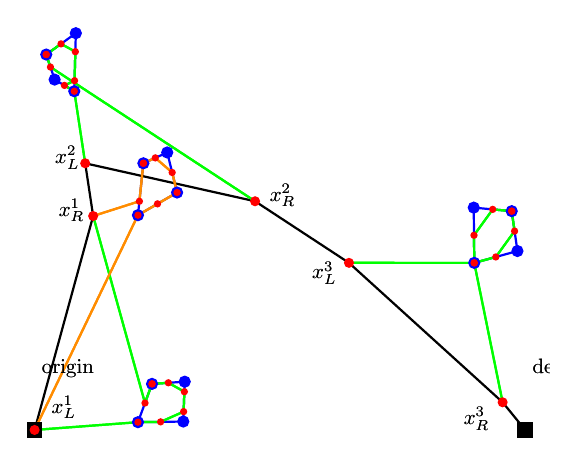
\begin{tikzpicture}

\definecolor{color0}{rgb}{1,0.549019607843137,0}

\begin{axis}[
hide x axis,
hide y axis,
scaled x ticks=manual:{}{\pgfmathparse{#1}},
scaled y ticks=manual:{}{\pgfmathparse{#1}},
tick align=outside,
x grid style={white!69.0196078431373!black},
xmajorticks=false,
xmin=-5, xmax=105,
xtick style={color=black},
xticklabels={},
y grid style={white!69.0196078431373!black},
ymajorticks=false,
ymin=-5, ymax=75,
ytick style={color=black},
yticklabels={}
]
\path [draw=blue, thick]
(axis cs:21.0696182692914,1.38670279952717)
--(axis cs:30.306045132353,1.50447958089156);

\path [draw=blue, thick]
(axis cs:21.0696182692914,1.38670279952717)
--(axis cs:23.9355243392435,8.22107815581281);

\path [draw=blue, thick]
(axis cs:30.306045132353,1.50447958089156)
--(axis cs:30.6007400849981,8.61180925900065);

\path [draw=blue, thick]
(axis cs:23.9355243392435,8.22107815581281)
--(axis cs:30.6007400849981,8.61180925900065);

\path [draw=blue, thick]
(axis cs:4.08370396767994,62.5193171258523)
--(axis cs:8.09069545603466,60.4417973648425);

\path [draw=blue, thick]
(axis cs:4.08370396767994,62.5193171258523)
--(axis cs:2.37426610997379,66.9905560181573);

\path [draw=blue, thick]
(axis cs:8.09069545603466,60.4417973648425)
--(axis cs:8.40433589338944,70.7975020391092);

\path [draw=blue, thick]
(axis cs:2.37426610997379,66.9905560181573)
--(axis cs:8.40433589338944,70.7975020391092);

\path [draw=blue, thick]
(axis cs:21.0664581490033,38.3255279820558)
--(axis cs:29.0472438012912,42.369596955967);

\path [draw=blue, thick]
(axis cs:21.0664581490033,38.3255279820558)
--(axis cs:22.1750046919912,47.5858849832036);

\path [draw=blue, thick]
(axis cs:29.0472438012912,42.369596955967)
--(axis cs:27.0356718607916,49.5164362980235);

\path [draw=blue, thick]
(axis cs:22.1750046919912,47.5858849832036)
--(axis cs:27.0356718607916,49.5164362980235);

\path [draw=blue, thick]
(axis cs:89.6170857784204,29.8130206242151)
--(axis cs:98.4204942730176,31.9280359170996);

\path [draw=blue, thick]
(axis cs:89.6170857784204,29.8130206242151)
--(axis cs:89.5168058385155,39.6742972814671);

\path [draw=blue, thick]
(axis cs:98.4204942730176,31.9280359170996)
--(axis cs:97.2556927544101,39.0446066906692);

\path [draw=blue, thick]
(axis cs:89.5168058385155,39.6742972814671)
--(axis cs:97.2556927544101,39.0446066906692);

\path [draw=black, thick]
(axis cs:0,0)
--(axis cs:0,0)
--(axis cs:11.9384375817266,38.1768740390765)
--(axis cs:10.3131414759248,47.5858849832036)
--(axis cs:44.9451427093311,40.8090894507933)
--(axis cs:64.0827735142413,29.8198845110857)
--(axis cs:95.4029040306271,4.93918065109767)
--(axis cs:100,0);
\path [draw=green, thick]
(axis cs:0,0)
--(axis cs:21.0696182692914,1.38670279952717)
--(axis cs:25.6878317008222,1.44559119020937)
--(axis cs:30.3792241725836,3.26938108252212)
--(axis cs:30.5265716489061,6.82304592157666)
--(axis cs:27.2681322121208,8.41644370740673)
--(axis cs:23.9355243392435,8.22107815581281)
--(axis cs:23.9355243392435,8.22107815581281)
--(axis cs:22.5025713042674,4.80389047767)
--(axis cs:11.9384375817266,38.1768740390765);
\path [draw=color0, thick]
(axis cs:0,0)
--(axis cs:21.0664581490033,38.3255279820558)
--(axis cs:25.0568509751472,40.3475624690114)
--(axis cs:29.0472438012912,42.369596955967)
--(axis cs:28.0414578310414,45.9430166269952)
--(axis cs:24.6053382763914,48.5511606406136)
--(axis cs:22.1750046919912,47.5858849832036)
--(axis cs:22.1750046919912,47.5858849832036)
--(axis cs:21.3637623976544,40.8090894507933)
--(axis cs:11.9384375817266,38.1768740390765);
\path [draw=green, thick]
(axis cs:0,0)
--(axis cs:21.0696182692914,1.38670279952717)
--(axis cs:25.6878317008222,1.44559119020937)
--(axis cs:30.3792241725836,3.26938108252212)
--(axis cs:30.5265716489061,6.82304592157666)
--(axis cs:27.2681322121208,8.41644370740673)
--(axis cs:23.9355243392435,8.22107815581281)
--(axis cs:23.9355243392435,8.22107815581281)
--(axis cs:22.5025713042674,4.80389047767)
--(axis cs:11.9384375817266,38.1768740390765);
\path [draw=color0, thick]
(axis cs:0,0)
--(axis cs:21.0664581490033,38.3255279820558)
--(axis cs:25.0568509751472,40.3475624690114)
--(axis cs:29.0472438012912,42.369596955967)
--(axis cs:28.0414578310414,45.9430166269952)
--(axis cs:24.6053382763914,48.5511606406136)
--(axis cs:22.1750046919912,47.5858849832036)
--(axis cs:22.1750046919912,47.5858849832036)
--(axis cs:21.3637623976544,40.8090894507933)
--(axis cs:11.9384375817266,38.1768740390765);
\path [draw=green, thick]
(axis cs:10.3131414759248,47.5858849832036)
--(axis cs:8.09069545603467,60.4417973648425)
--(axis cs:6.08719971185731,61.4805572453474)
--(axis cs:8.1475539671049,62.3191380350312)
--(axis cs:8.30437418578229,67.4969903721645)
--(axis cs:5.38930100168162,68.8940290286332)
--(axis cs:2.37426610997379,66.9905560181573)
--(axis cs:2.3742661099738,66.9905560181572)
--(axis cs:3.22898503882687,64.7549365720048)
--(axis cs:44.9451427093311,40.8090894507933);
\path [draw=green, thick]
(axis cs:10.3131414759248,47.5858849832036)
--(axis cs:8.09069545603467,60.4417973648425)
--(axis cs:6.08719971185731,61.4805572453474)
--(axis cs:8.1475539671049,62.3191380350312)
--(axis cs:8.30437418578229,67.4969903721645)
--(axis cs:5.38930100168162,68.8940290286332)
--(axis cs:2.37426610997379,66.9905560181573)
--(axis cs:2.3742661099738,66.9905560181572)
--(axis cs:3.22898503882687,64.7549365720048)
--(axis cs:44.9451427093311,40.8090894507933);
\path [draw=green, thick]
(axis cs:64.0827735142413,29.8198845110857)
--(axis cs:89.6170857784204,29.8130206242151)
--(axis cs:94.018790025719,30.8705282706573)
--(axis cs:97.8380935137139,35.4863213038844)
--(axis cs:97.2556927544101,39.0446066906692)
--(axis cs:97.25569275441,39.0446066906692)
--(axis cs:93.3862492964628,39.3594519860681)
--(axis cs:89.5669458084679,34.7436589528409)
--(axis cs:89.6170857784204,29.8130206242149)
--(axis cs:95.4029040306271,4.93918065109767);
\path [draw=green, thick]
(axis cs:64.0827735142413,29.8198845110857)
--(axis cs:89.6170857784204,29.8130206242151)
--(axis cs:94.018790025719,30.8705282706573)
--(axis cs:97.8380935137139,35.4863213038844)
--(axis cs:97.2556927544101,39.0446066906692)
--(axis cs:97.25569275441,39.0446066906692)
--(axis cs:93.3862492964628,39.3594519860681)
--(axis cs:89.5669458084679,34.7436589528409)
--(axis cs:89.6170857784204,29.8130206242149)
--(axis cs:95.4029040306271,4.93918065109767);
\addplot [draw=blue, fill=blue, mark=*, only marks]
table{%
x  y
21.0696182692914 1.38670279952717
30.306045132353 1.50447958089156
23.9355243392435 8.22107815581281
30.6007400849981 8.61180925900065
};
\addplot [draw=blue, fill=blue, mark=*, only marks]
table{%
x  y
4.08370396767994 62.5193171258523
8.09069545603466 60.4417973648425
2.37426610997379 66.9905560181573
8.40433589338944 70.7975020391092
};
\addplot [draw=blue, fill=blue, mark=*, only marks]
table{%
x  y
21.0664581490033 38.3255279820558
29.0472438012912 42.369596955967
22.1750046919912 47.5858849832036
27.0356718607916 49.5164362980235
};
\addplot [draw=blue, fill=blue, mark=*, only marks]
table{%
x  y
89.6170857784204 29.8130206242151
98.4204942730176 31.9280359170996
89.5168058385155 39.6742972814671
97.2556927544101 39.0446066906692
};
\addplot [semithick, red, mark=*, mark size=1, mark options={solid}, only marks]
table {%
25.6878317008222 1.44559119020937
21.0696182692914 1.38670279952717
23.9355243392435 8.22107815581281
22.5025713042674 4.80389047767
30.3792241725836 3.26938108252212
30.5265716489061 6.82304592157666
27.2681322121208 8.41644370740673
23.9355243392435 8.22107815581281
8.09069545603467 60.4417973648425
6.08719971185731 61.4805572453474
2.3742661099738 66.9905560181572
3.22898503882687 64.7549365720048
8.1475539671049 62.3191380350312
8.30437418578229 67.4969903721645
5.38930100168162 68.8940290286332
2.37426610997379 66.9905560181573
21.0664581490033 38.3255279820558
25.0568509751472 40.3475624690114
22.1750046919912 47.5858849832036
21.3637623976544 40.8090894507933
29.0472438012912 42.369596955967
28.0414578310414 45.9430166269952
24.6053382763914 48.5511606406136
22.1750046919912 47.5858849832036
89.6170857784204 29.8130206242151
94.018790025719 30.8705282706573
89.5669458084679 34.7436589528409
89.6170857784204 29.8130206242149
97.8380935137139 35.4863213038844
97.2556927544101 39.0446066906692
97.25569275441 39.0446066906692
93.3862492964628 39.3594519860681
};
\addplot [semithick, black, opacity=1, mark=square*, mark size=2.5, mark options={solid}, only marks]
table {%
0 0
100 0
};
\addplot [semithick, red, opacity=1, mark=*, mark size=1.5, mark options={solid}, only marks]
table {%
0 0
11.9384375817266 38.1768740390765
10.313141475924828 47.585884983203592
44.9451427093311 40.8090894507933
64.082773514241339 29.819884511085665
95.4029040306271 4.93918065109767
};
\draw (0,10) node[
  scale=0.75,
  anchor=base west,
  text=black,
  rotate=0.0
]{origin};
\draw (0,10) node[
  scale=0.75,
  anchor=base west,
  text=black,
  rotate=0.0
]{origin};
\draw (axis cs:3.4384375817266,38.1768740390765) node[
  scale=0.75,
  anchor=base west,
  text=black,
  rotate=0.0
]{$x_R^1$};
\draw (axis cs:2,3) node[
  scale=0.75,
  anchor=base west,
  text=black,
  rotate=0.0
]{$x_L^1$};
\draw (axis cs:3.4384375817266,38.1768740390765) node[
  scale=0.75,
  anchor=base west,
  text=black,
  rotate=0.0
]{$x_R^1$};
\draw (axis cs:2,3) node[
  scale=0.75,
  anchor=base west,
  text=black,
  rotate=0.0
]{$x_L^1$};
\draw (axis cs:46.4451427093311,40.8090894507933) node[
  scale=0.75,
  anchor=base west,
  text=black,
  rotate=0.0
]{$x_R^2$};
\draw (axis cs:2.7,47.5858849832036) node[
  scale=0.75,
  anchor=base west,
  text=black,
  rotate=0.0
]{$x_L^2$};
\draw (axis cs:46.4451427093311,40.8090894507933) node[
  scale=0.75,
  anchor=base west,
  text=black,
  rotate=0.0
]{$x_R^2$};
\draw (axis cs:2.7,47.5858849832036) node[
  scale=0.75,
  anchor=base west,
  text=black,
  rotate=0.0
]{$x_L^2$};
\draw (axis cs:86,1) node[
  scale=0.75,
  anchor=base west,
  text=black,
  rotate=0.0
]{$x_R^3$};
\draw (axis cs:55.0827735142413,27) node[
  scale=0.75,
  anchor=base west,
  text=black,
  rotate=0.0
]{$x_L^3$};
\draw (axis cs:86,1) node[
  scale=0.75,
  anchor=base west,
  text=black,
  rotate=0.0
]{$x_R^3$};
\draw (axis cs:55.0827735142413,27) node[
  scale=0.75,
  anchor=base west,
  text=black,
  rotate=0.0
]{$x_L^3$};
\draw (100, 10) node[
  scale=0.75,
  anchor=base west,
  text=black,
  rotate=0.0
]{dest};
\draw (100, 10) node[
  scale=0.75,
  anchor=base west,
  text=black,
  rotate=0.0
]{dest};
\end{axis}
\end{tikzpicture}
\subcaption{[a]}
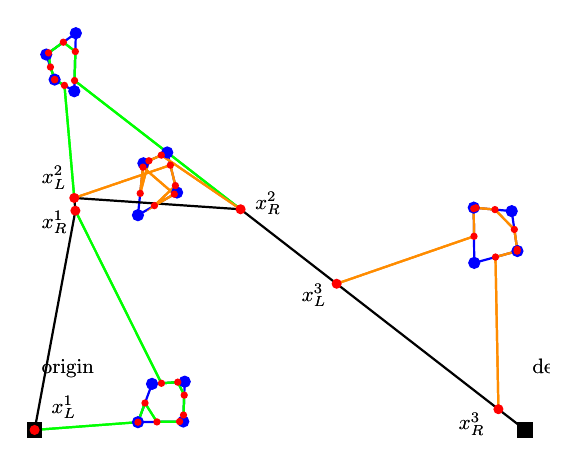
\begin{tikzpicture}
\definecolor{color0}{rgb}{1,0.549019607843137,0}
\begin{axis}[
hide x axis,
hide y axis,
scaled x ticks=manual:{}{\pgfmathparse{#1}},
scaled y ticks=manual:{}{\pgfmathparse{#1}},
tick align=outside,
x grid style={white!69.0196078431373!black},
xmajorticks=false,
xmin=-5, xmax=105,
xtick style={color=black},
xticklabels={},
y grid style={white!69.0196078431373!black},
ymajorticks=false,
ymin=-5, ymax=75,
ytick style={color=black},
yticklabels={}
]
\path [draw=blue, thick]
(axis cs:21.0696182692914,1.38670279952717)
--(axis cs:30.306045132353,1.50447958089156);

\path [draw=blue, thick]
(axis cs:21.0696182692914,1.38670279952717)
--(axis cs:23.9355243392435,8.22107815581281);

\path [draw=blue, thick]
(axis cs:30.306045132353,1.50447958089156)
--(axis cs:30.6007400849981,8.61180925900065);

\path [draw=blue, thick]
(axis cs:23.9355243392435,8.22107815581281)
--(axis cs:30.6007400849981,8.61180925900065);

\path [draw=blue, thick]
(axis cs:4.08370396767994,62.5193171258523)
--(axis cs:8.09069545603466,60.4417973648425);

\path [draw=blue, thick]
(axis cs:4.08370396767994,62.5193171258523)
--(axis cs:2.37426610997379,66.9905560181573);

\path [draw=blue, thick]
(axis cs:8.09069545603466,60.4417973648425)
--(axis cs:8.40433589338944,70.7975020391092);

\path [draw=blue, thick]
(axis cs:2.37426610997379,66.9905560181573)
--(axis cs:8.40433589338944,70.7975020391092);

\path [draw=blue, thick]
(axis cs:21.0664581490033,38.3255279820558)
--(axis cs:29.0472438012912,42.369596955967);

\path [draw=blue, thick]
(axis cs:21.0664581490033,38.3255279820558)
--(axis cs:22.1750046919912,47.5858849832036);

\path [draw=blue, thick]
(axis cs:29.0472438012912,42.369596955967)
--(axis cs:27.0356718607916,49.5164362980235);

\path [draw=blue, thick]
(axis cs:22.1750046919912,47.5858849832036)
--(axis cs:27.0356718607916,49.5164362980235);

\path [draw=blue, thick]
(axis cs:89.6170857784204,29.8130206242151)
--(axis cs:98.4204942730176,31.9280359170996);

\path [draw=blue, thick]
(axis cs:89.6170857784204,29.8130206242151)
--(axis cs:89.5168058385155,39.6742972814671);

\path [draw=blue, thick]
(axis cs:98.4204942730176,31.9280359170996)
--(axis cs:97.2556927544101,39.0446066906692);

\path [draw=blue, thick]
(axis cs:89.5168058385155,39.6742972814671)
--(axis cs:97.2556927544101,39.0446066906692);

\path [draw=black, thick]
(axis cs:0,0)
--(axis cs:5.19517108668237e-05,5.19721988422751e-05)
--(axis cs:8.31804668177588,39.1256215879103)
--(axis cs:8.0902667404291,41.3992381927182)
--(axis cs:41.9928361091472,39.3784823234059)
--(axis cs:61.5718673452208,26.0879192386296)
--(axis cs:94.5456634712005,3.70413789044963)
--(axis cs:100,0);
\path [draw=green, thick]
(axis cs:5.19517108668237e-05,5.19721988422751e-05)
--(axis cs:21.0696185355958,1.3867034345879)
--(axis cs:22.5025656416375,4.80387697389931)
--(axis cs:24.9379489929542,1.43602918392242)
--(axis cs:29.5561397992636,1.49491728610282)
--(axis cs:30.353931133669,2.65937414309857)
--(axis cs:30.5012780269027,6.21302491945877)
--(axis cs:29.1826401424249,8.52867680295897)
--(axis cs:25.850065249296,8.33331318471784)
--(axis cs:8.31804668177588,39.1256215879103);
\path [draw=green, thick]
(axis cs:5.19517108668237e-05,5.19721988422751e-05)
--(axis cs:21.0696185355958,1.3867034345879)
--(axis cs:22.5025656416375,4.80387697389931)
--(axis cs:24.9379489929542,1.43602918392242)
--(axis cs:29.5561397992636,1.49491728610282)
--(axis cs:30.353931133669,2.65937414309857)
--(axis cs:30.5012780269027,6.21302491945877)
--(axis cs:29.1826401424249,8.52867680295897)
--(axis cs:25.850065249296,8.33331318471784)
--(axis cs:8.31804668177588,39.1256215879103);
\path [draw=green, thick]
(axis cs:8.0902667404291,41.3992381927182)
--(axis cs:6.08717590107675,61.4805695906112)
--(axis cs:4.0837005407278,62.5193189026369)
--(axis cs:4.08369465698464,62.5193414790879)
--(axis cs:3.22897670117108,64.7549583801393)
--(axis cs:2.84174575638185,67.2856885528858)
--(axis cs:5.85674978390742,69.1891420779693)
--(axis cs:8.3052804744899,67.5269139951667)
--(axis cs:8.14846106263484,62.3490882974996)
--(axis cs:41.9928361091472,39.3784823234059);
\path [draw=color0, thick]
(axis cs:8.0902667404291,41.3992381927182)
--(axis cs:27.6728191506586,47.2527393224256)
--(axis cs:28.7000788954416,43.6030262742796)
--(axis cs:24.4315739690114,40.0307185577996)
--(axis cs:28.4696719165738,42.0769264544708)
--(axis cs:22.0922910532811,46.8949281369037)
--(axis cs:21.5323008920902,42.2169930131509)
--(axis cs:23.3011399504012,48.0331614224841)
--(axis cs:25.830886920397,49.0379219151249)
--(axis cs:41.9928361091472,39.3784823234059);
\path [draw=green, thick]
(axis cs:8.0902667404291,41.3992381927182)
--(axis cs:6.08717590107675,61.4805695906112)
--(axis cs:4.0837005407278,62.5193189026369)
--(axis cs:4.08369465698464,62.5193414790879)
--(axis cs:3.22897670117108,64.7549583801393)
--(axis cs:2.84174575638185,67.2856885528858)
--(axis cs:5.85674978390742,69.1891420779693)
--(axis cs:8.3052804744899,67.5269139951667)
--(axis cs:8.14846106263484,62.3490882974996)
--(axis cs:41.9928361091472,39.3784823234059);
\path [draw=color0, thick]
(axis cs:8.0902667404291,41.3992381927182)
--(axis cs:27.6728191506586,47.2527393224256)
--(axis cs:28.7000788954416,43.6030262742796)
--(axis cs:24.4315739690114,40.0307185577996)
--(axis cs:28.4696719165738,42.0769264544708)
--(axis cs:22.0922910532811,46.8949281369037)
--(axis cs:21.5323008920902,42.2169930131509)
--(axis cs:23.3011399504012,48.0331614224841)
--(axis cs:25.830886920397,49.0379219151249)
--(axis cs:41.9928361091472,39.3784823234059);
\path [draw=color0, thick]
(axis cs:61.5718673452208,26.0879192386296)
--(axis cs:89.5688132333832,34.5600210912317)
--(axis cs:89.5186458802408,39.4933522137777)
--(axis cs:89.9608257385526,39.6381686810341)
--(axis cs:93.8383627815696,39.3226648342931)
--(axis cs:97.7899505784608,35.7804594900926)
--(axis cs:98.374626227098,32.2082752452751)
--(axis cs:98.3537907014276,31.9120104112867)
--(axis cs:93.9472998319943,30.8533527808329)
--(axis cs:94.5456634712005,3.70413789044963);
\path [draw=color0, thick]
(axis cs:61.5718673452208,26.0879192386296)
--(axis cs:89.5688132333832,34.5600210912317)
--(axis cs:89.5186458802408,39.4933522137777)
--(axis cs:89.9608257385526,39.6381686810341)
--(axis cs:93.8383627815696,39.3226648342931)
--(axis cs:97.7899505784608,35.7804594900926)
--(axis cs:98.374626227098,32.2082752452751)
--(axis cs:98.3537907014276,31.9120104112867)
--(axis cs:93.9472998319943,30.8533527808329)
--(axis cs:94.5456634712005,3.70413789044963);
\addplot [draw=blue, fill=blue, mark=*, only marks]
table{%
x  y
21.0696182692914 1.38670279952717
30.306045132353 1.50447958089156
23.9355243392435 8.22107815581281
30.6007400849981 8.61180925900065
};
\addplot [draw=blue, fill=blue, mark=*, only marks]
table{%
x  y
4.08370396767994 62.5193171258523
8.09069545603466 60.4417973648425
2.37426610997379 66.9905560181573
8.40433589338944 70.7975020391092
};
\addplot [draw=blue, fill=blue, mark=*, only marks]
table{%
x  y
21.0664581490033 38.3255279820558
29.0472438012912 42.369596955967
22.1750046919912 47.5858849832036
27.0356718607916 49.5164362980235
};
\addplot [draw=blue, fill=blue, mark=*, only marks]
table{%
x  y
89.6170857784204 29.8130206242151
98.4204942730176 31.9280359170996
89.5168058385155 39.6742972814671
97.2556927544101 39.0446066906692
};
\addplot [semithick, red, mark=*, mark size=1, mark options={solid}, only marks]
table {%
24.9379489929542 1.43602918392242
29.5561397992636 1.49491728610282
21.0696185355958 1.3867034345879
22.5025656416375 4.80387697389931
30.353931133669 2.65937414309857
30.5012780269027 6.21302491945877
29.1826401424249 8.52867680295897
25.850065249296 8.33331318471784
6.08717590107675 61.4805695906112
4.0837005407278 62.5193189026369
4.08369465698464 62.5193414790879
3.22897670117108 64.7549583801393
8.3052804744899 67.5269139951667
8.14846106263484 62.3490882974996
2.84174575638185 67.2856885528858
5.85674978390742 69.1891420779693
24.4315739690114 40.0307185577996
28.4696719165738 42.0769264544708
22.0922910532811 46.8949281369037
21.5323008920902 42.2169930131509
27.6728191506586 47.2527393224256
28.7000788954416 43.6030262742796
23.3011399504012 48.0331614224841
25.830886920397 49.0379219151249
98.3537907014276 31.9120104112867
93.9472998319943 30.8533527808329
89.5688132333832 34.5600210912317
89.5186458802408 39.4933522137777
97.7899505784608 35.7804594900926
98.374626227098 32.2082752452751
89.9608257385526 39.6381686810341
93.8383627815696 39.3226648342931
};

\addplot [semithick, black, opacity=1, mark=square*, mark size=2.5, mark options={solid}, only marks]
table {%
0 0
100 0
};
\addplot [semithick, red, opacity=1, mark=*, mark size=1.5, mark options={solid}, only marks]
table {%
5.19517108668237e-05 5.19721988422751e-05
8.31804668177588 39.1256215879103
8.0902667404291044 41.399238192718173
41.9928361091472 39.3784823234059
61.571867345220838 26.087919238629631
94.5456634712005 3.70413789044963
};
\draw (0, 10) node[
  scale=0.75,
  anchor=base west,
  text=black,
  rotate=0.0
]{origin};
\draw (axis cs:2,3) node[
  scale=0.75,
  anchor=base west,
  text=black,
  rotate=0.0
]{$x_L^1$};
\draw (axis cs:0,36) node[
  scale=0.75,
  anchor=base west,
  text=black,
  rotate=0.0
]{$x_R^1$};
\draw (axis cs:0,44) node[
  scale=0.75,
  anchor=base west,
  text=black,
  rotate=0.0
]{$x_L^2$};
\draw (axis cs:43.4928361091472,39.3784823234059) node[
  scale=0.75,
  anchor=base west,
  text=black,
  rotate=0.0
]{$x_R^2$};
\draw (axis cs:53,23) node[
  scale=0.75,
  anchor=base west,
  text=black,
  rotate=0.0
]{$x_L^3$};
\draw (axis cs:85,0) node[
  scale=0.75,
  anchor=base west,
  text=black,
  rotate=0.0
]{$x_R^3$};
\draw (100,10) node[
  scale=0.75,
  anchor=base west,
  text=black,
  rotate=0.0
]{dest};
\draw (0, 10) node[
  scale=0.75,
  anchor=base west,
  text=black,
  rotate=0.0
]{origin};
\draw (axis cs:2,3) node[
  scale=0.75,
  anchor=base west,
  text=black,
  rotate=0.0
]{$x_L^1$};
\draw (axis cs:0,36) node[
  scale=0.75,
  anchor=base west,
  text=black,
  rotate=0.0
]{$x_R^1$};
\draw (axis cs:0,44) node[
  scale=0.75,
  anchor=base west,
  text=black,
  rotate=0.0
]{$x_L^2$};
\draw (axis cs:43.4928361091472,39.3784823234059) node[
  scale=0.75,
  anchor=base west,
  text=black,
  rotate=0.0
]{$x_R^2$};
\draw (axis cs:53,23) node[
  scale=0.75,
  anchor=base west,
  text=black,
  rotate=0.0
]{$x_L^3$};
\draw (axis cs:85,0) node[
  scale=0.75,
  anchor=base west,
  text=black,
  rotate=0.0
]{$x_R^3$};
\draw (100,10) node[
  scale=0.75,
  anchor=base west,
  text=black,
  rotate=0.0
]{dest};
\end{axis}
\end{tikzpicture}
\subcaption{[b]}
\caption{Example of feasible solution [a] and optimal solution [b] for a problem instance with 4 graphs and 2 drones.}
\label{fig:illustrative}
\end{figure}
\noindent
Figure \ref{fig:illustrative} shows an example of the notation over a configuration with four target graphs that have four nodes and four edges. Here, it is supposed that the number of available drones is two. %: one with six nodes and 7 edges and the other one with four nodes and edges%. 
\LA{In particular, figure \ref{fig:illustrative}[a] represents a feasible solution of the problem for this configuration.
The mothership begins at its starting point $orig$ which coincides with the first launching point $x_L^1$ where two drones (the green one and the orange one) are launched to visit two graphs. There, each drone follows a route (represented by the orange and green paths) that ensures the coverage of \RE{one half of the length of} each edge of the graph. The red dots on the visited graphs are the intermediate points $R^{e_g}$ and $L^{e_g}$ used by the drones in their visit to the edges of the different graphs. After finishing the visit of the first two graphs\RE{,} the drones return to the point $x_R^1$. The mothership moves from this point to the second launching point $x_L^2$ from where only one drone (the green one) is launched to visit the third graph. Once this graph is visited, the drone returns to the mothership at the rendezvous point $x_R^2$. Finally, the mothership moves to point $x_L^3$ from where one drone is launched for the last visit to the fourth graph. Then, the drone is retrieved by the mothership at point $x_R^3$ and then the mothership ends its route at the destination point $dest$.\\
Figure \ref{fig:illustrative}[b] represents the optimal solution for the same instance of the problem. We can observe that in this case from the first launching point $x_L^1$ only one drone is launched, while from the second $x_L^2$ two drones are launched to visit the second and the third graph. The different position in the space of this latter point, with respect to the feasible solution reported in figure \ref{fig:illustrative}[a] whose total time is 158.36, ensures that the total travelled time of the optimal solution equals to 152.39, which is shorter.}


% \JP{ ************************ 

% TO BE INSERTED: An example showing the notation with a figure...  Please Carlos insert something similar to what we use in the previous paper (JUSTO dixit)

%      ************************}
\noindent
To include the definition of these paths in our mathematical programming formulation\RE{,} we need to make decisions to choose:
\begin{itemize}
    \item The optimal assignment of drones for visiting graphs in a given \RE{operation $o$}.
    \item The order to visit the edges of each graph in its corresponding \RE{operation}.
\end{itemize}

% Binary variables
% Thus, to this end one can define the following binary variables:

\subsubsection*{Drone Constraints}
\noindent
We model the route that the drone follows by using the binary variables $u^{e_go}$, $z^{e_ge^\prime_g}$ and $v^{e_go}$ defined in Table \ref{table:t2}.


% \begin{itemize}
%   \item $u^{{e_g}td} = 1$ if the visit of graph $g$ is done at stage $t$ by the drone $d$ and it starts from edge $e_g$.
%   \item $v^{{e_g}td}= 1$ if the visit of graph $g$ that is done by drone $d$ at stage $t$ finishes in the edge $e_g$.
%   \item $z^{e_ge'_g}= 1$ if the drone moves from edge $e_g$ to $e'_g$ while visiting the graph $g$.
% \end{itemize}

% By using these binary variables, we can model the route that follows the drone:
\begin{align}
    % \sum_{g\in \mathcal G}\sum_{e_g\in E_g} \sum_{d\in\mathcal D} u^{e_gtd} & \leq 1, &\forall t\in \mathcal T, \label{st:DEnt}\\%\tag{DEn}\\
    % \sum_{g\in\mathcal G}\sum_{e_g\in E_g} \sum_{d\in\mathcal D} v^{e_gtd} & \leq 1, &\forall t\in \mathcal T, \label{st:DExt}\\%\tag{DEx}\\
    \sum_{g\in \mathcal G}\sum_{e_g\in E_g}  u^{e_go} & \leq \RE{|\mathcal D|}, &\forall o\in \mathcal O,\label{st:DEnt}\\
    \sum_{g\in \mathcal G}\sum_{e_g\in E_g}  v^{e_go} & \leq \RE{|\mathcal D|}, &\forall o\in \mathcal O,\label{st:DExt} \\
    \sum_{e_g\in E_g} \sum_{o\in \mathcal O} u^{e_go} & = 1, &\forall g\in\mathcal G, \label{st:DEng}\\%\tag{D
    \sum_{e_g\in E_g} \sum_{o\in \mathcal O} v^{e_go} & = 1, &\forall g\in\mathcal G, \label{st:DExg}\\%\tag{D
    \sum_{e_g\in E_g} u^{e_go} & = \sum_{e_g\in E_g} v^{e_go}, &\forall g\in\mathcal G, \forall o\in \mathcal O, \label{st:Duv}\\%\tag{D
     \sum_{o\in \mathcal O} u^{e_go} + \sum_{e^\prime_g\in E_g} z_g^{e^\prime_ge_g} & = \mu^{e_g}, &\forall e_g\in E_g:g\in\mathcal G, \label{st:DInu}\\
     \sum_{o\in \mathcal O} v^{e_go} + \sum_{e^\prime_g\in E_g} z_g^{e_ge^\prime_g} & = \mu^{e_g}, &\forall e_g\in E_g:g\in\mathcal G. \label{st:DInv}
\end{align}

\noindent 
\RE{Inequalities \eqref{st:DEnt} and \eqref{st:DExt} state that a drone visits at most one graph $g$ at operation $o$.}  Constraints \eqref{st:DEng} and \eqref{st:DExg} assure that each graph is visited at some \RE{operation $o$} by some drone. Equations \eqref{st:Duv} ensure that the \RE{action} of entering and exiting from the graph $g$ occurs in the same \RE{operation $o$} and is done by the same drone. Constraints \eqref{st:DInu} state that if \RE{an} edge $e$ of graph $g$ is visited by a drone, one of two alternative situations must occur: either $e$ is the first edge of graph $g$ visited by the drone at \RE{operation $o$}, or edge $e$ is visited by the drone after visiting another edge $e^\prime$ of graph $g$. Similarly, constraints \eqref{st:DInv} state that if \RE{an} edge $e$ of graph $g$ is visited by a drone, either $e$ is the last edge of graph $g$ visited by the drone at \RE{operation $o$}, or the drone must move to another edge $e^\prime$ of graph $g$ after visiting edge $e$.

\subsubsection*{Distance and Time Constraints}
\noindent
The goal of the \AMD\xspace is to find a feasible solution that minimizes the total \RE{time} traveled by the mothership. To account for the different distances \RE{between} the decision variables of the model we need to set the continuous variables $d_L^{e_go}$, $d^{e_g}$, $d^{e_ge^\prime_g}$, $d_R^{e_go}$, $d_{RL}^o$ and $d_{LR}^o$, defined in Table \ref{table:t2}. This can be done by means of the following constraints:

\begin{align*}
\|x_L^o- R^{e_g}\| & \leq  d_L^{e_go},  &\forall e_g:g\in \mathcal{G}, \:\:\forall o\in \mathcal O, \tag{Drone DIST$_{1}$-CO} \label{eq:drone-d1-async-CO}\\
\|R^{e_g}- L^{e_g}\| & \leq  d^{e_g},  &\forall e_g:g\in \mathcal{G}, \tag{Drone DIST$_{2}$-CO} \label{eq:drone-d2-async-CO}\\
\|R^{e_g}- L^{e'_g}\| & \leq  d^{e_ge'_g}, &\forall e_g\neq e_g'\in E_g:g\in \mathcal{G}, \tag{Drone DIST$_{3}$-CO} \label{eq:drone-d3-async-CO}\\
\|L^{e_g}- x_R^o\| & \leq  d_R^{e_o}, &\forall e_g:g\in \mathcal{G},\:\:\forall o\in \mathcal O. \tag{Drone DIST$_{4}$-CO} \label{eq:drone-d4-async-CO}\\\\
\|orig - x_L^1\| & \leq d_{orig}, \tag{Mothership DIST$_1$-CO}\label{eq:mothership-d1-async-CO}\\
\|x_L^o - x_R^{o}\| & \leq d_{LR}^{o}, &\forall o\in\mathcal O, \tag{Mothership DIST$_{2}$-CO}\label{eq:mothership-d3-async-CO}\\
\|x_R^o - x_L^{o+1}\| & \leq d_{RL}^{o}, &\forall t\in\mathcal O:o<|\mathcal O|, \tag{Mothership DIST$_{3}$-CO}\label{eq:mothership-d4-async-CO}\\
\|x_R^{|\mathcal O|} - dest\| & \leq d_{dest}. \tag{Mothership DIST$_4$-CO}\label{eq:mothership-d6-async-CO}
\end{align*}

\noindent
All the variables modelling \RE{the} distances covered by drones, namely $d_L^{e_go}$, $d^{e_g}$, $d^{e_g'e_g}$ and $d_R^{e_go}$,  as well as those modelling the distance travelled by the mothership, namely $d_{orig}$, $d_{LL}^o$, $d_{LR}^o$, $d_{RL}^o$, $d_{RR}^o$ and $d_{dest}$, are defined in \JP{Table \ref{table:t2}.} 
 
 
 
\begin{comment}
\begin{align*}
\|x_L^o- R^{e_g}\| & \leq  d_L^{e_go},  &\quad \forall e_g:g\in \mathcal{G}, \forall o\in \mathcal O, \tag{DIST$_{1}$-o} \label{eq:d1}\\
\|R^{e_g}- L^{e_g}\| & \leq  d^{e_g},  &\quad \forall e_g:g\in \mathcal{G}, \tag{DIST$_{2}$-o} \label{eq:d2}\\
\|R^{e_g}- L^{e^\prime_g}\| & \leq  d^{e_ge^\prime_g}, &\quad \forall e_g\neq e_g'\in E_g:g\in \mathcal{G}, \tag{DIST$_{3}$-o} \label{eq:d3}\\
\|L^{e_g}- x_R^o\| & \leq  d_R^{e_go}, &\quad \forall e_g:g\in \mathcal{G},\forall o\in \mathcal O, \tag{DIST$_{4}$-o} \label{eq:d4}\\
\|x_R^o- x_L^{o+1}\| & \leq  d_{RL}^o, & \quad \forall o\in \mathcal O\CV{\setminus |\mathcal O|}, \tag{DIST$_{5}$-o} \label{eq:d5}\\
\|x_L^o- x_R^o\| & \leq  d_{LR}^o, & \quad \forall o\in \mathcal O. \tag{DIST$_{6}$-o} \label{eq:d6}\\
\end{align*}
\end{comment}

\RE{
\noindent
In order to compute the maximum time spent by a drone to visit a graph $g \in \mathcal G$ associated with operation $o \:\:\ \forall o \in \mathcal O$, we introduce the following constraints:

\begin{equation}\tag{Time$_D^o$}
time_D^o \geq \frac{1}{v_D}\left(\sum_{e_g\in E_g} u^{e_go}d_L^{e_go} + \sum_{e_g, e^\prime_g\in E_g}z^{e_ge^\prime_g}d^{e_ge^\prime_g} + \sum_{e_g\in E_g} \mu^{e_g}d^{e_g} + \sum_{e_g\in E_g} v^{e_go}d_R^{e_go}\right) - \CV{N_D}(1 - \sum_{e_g\in E_g} u^{e_go}). %\:\: \forall g \in \mathcal G \:\: \forall o \in \mathcal O
\label{eq:timeD}
\end{equation}
\noindent
The first addend within the brackets accounts for the time spent by the drone to go from the launching point $x_L^o$ to the first retrieving point in the graph $R^{e_g}$. The second addend considers the time consumed by the drone to go from edge $e_g$ to $e_g'$ in the graph $g$. The third one computes the time required for traversing the required edges in $g$. The fourth one measures the time to travel from the last launching point $L^{e_g''}$ to the retrieving point $x_R^o$. \CV{Note that, in the special case where all edges must be visited, the third sum of the left-hand side of the \eqref{eq:timeD}, reduces to $\sum_{e_g\in E_g} d^{e_g}$ by setting all the $\mu^{e_g}$ variables equal to one.}

The \CV{\sout{big M} endurance} term in constraint (\ref{eq:timeD}) ensures that the constraint \textbf{becomes active} only when a graph $g$ is visited during operation $o$. \CV{The reader may observe that the endurance constraint \eqref{CAP} restricts the time spent by the drone to perform operation $o$ to be less than the endurance $N_D$. Therefore, the constant $N_D$ can be taken as bigM term in \eqref{eq:timeD}.}
\noindent
Note that, to deal with the bilinear terms of \eqref{eq:timeD}, we use McCormick's envelopes to linearize them by adding variables $p\geq 0$  representing the products and introducing the following constraints:
\begin{align*}
    p & \leq  M z, \\
    p & \leq  d, \\
    p & \geq m z, \\
    p & \geq d - M(1 - z),
\end{align*}
where $m$ and $M$ are, respectively, the lower and upper bounds of the distance variable $d$. These bounds will be adjusted for each bilinear term in Section \ref{bounds}.

\noindent
Constraints (\ref{eq:timeMO}) defines the time spent by the mothership to go from the launching point $x_L^o$ to the retrieving point $x_R^o$ associated with operation $o$.

\begin{equation}\tag{Time$_M^o$}
time_M^o = \frac{d_{LR}^o}{v_M}, \quad \forall o \in \mathcal O.
\label{eq:timeMO}
\end{equation}

\noindent
Thus, the overall time spent by the mothership to move from the origin to the destination can be expressed as follows:

\begin{equation}\tag{Time$_M$}
time_M = \frac{1}{v_M} (d_{orig} + \sum_{o \in \mathcal O} (d_{LR}^o + d_{RL}^o) + d_{dest}).
\label{eq:timeM}
\end{equation}



\subsubsection*{Coordination and Endurance Constraints}
\noindent
The coordination between the drones and the mothership must ensure that the maximum time $time_D^o$ spent by a drone to visit a graph $g$ at \RE{operation $o$} is less than or equal to the time that the mothership needs to move from the launching point to the retrieving point during \RE{operation $o$}. To this end, we need to define the following coordination constraint for each operation $o\in \mathcal O$:

\begin{equation}\tag{DCW-CO}\label{DCW}
time_D^o \leq time_M^o.
\end{equation}



\noindent
We can model the time endurance constraint for a particular \RE{operation $o\in \mathcal O$} by limiting the time traveled by the drone for this \RE{operation $o$}:

\begin{equation}\tag{Endurance-CO}\label{CAP}
    time_D^o \leq N_D.
\end{equation}


\subsubsection*{AMMDRPG-Complete Overlapping Formulation}
\noindent
Putting together all the constraints introduced before, the following formulation minimizes the \RE{total time} traveled by the mothership\RE{,} ensuring the coordination with the fleet of drones while guaranteeing the required coverage of the target graphs.
\begin{mini*}|s|
 {}{time_M}{}{} \label{AMMDRPG} \tag{AMMDRPG-Complete Overlapping}
  \addConstraint{\eqref{eq:alpha-E} \text{ or } \eqref{eq:alpha-G}}{}{}
  \addConstraint{\eqref{MTZ1}-\eqref{MTZ2}} \text{ or }  \eqref{SEC}
 \addConstraint{\eqref{st:DEnt}-\eqref{st:DInv}}{}{}
 \addConstraint{\eqref{eq:drone-d1-async-CO}-\eqref{eq:drone-d4-async-CO}}{}{} \addConstraint{\eqref{eq:mothership-d1-async-CO}-\eqref{eq:mothership-d6-async-CO}}{}{}
 \addConstraint{\eqref{eq:timeD}, \eqref{eq:timeMO}, \eqref{eq:timeM}}{}{}
 \addConstraint{\eqref{DCW}, \eqref{CAP}}{}{}
\end{mini*}

\noindent
The objective function accounts for the \RE{time} traveled by the mothership. Constraints \eqref{st:DEnt}-\eqref{st:DInv} models the route followed by the \RE{drones}, \eqref{MTZ1} - \eqref{MTZ2} \text{ or } \eqref{SEC} ensure that the displacement of \RE{a drone}  assigned to the target graph $g\in\mathcal G$ is a route, \eqref{eq:alpha-E} \text{ or } \eqref{eq:alpha-G} define what is required in each visit to a target graph. Constraints (\ref{eq:drone-d1-async-CO})-(\ref{eq:drone-d4-async-CO}) set the variables $d_L^{e_go}$, $d^{e_g}$, $d^{e_ge^\prime_g}$, $d_R^{e_go}$.
The mothership distances $d_{RL}^o$ and $d_{LR}^o$, are defined by means of constraints (\ref{eq:mothership-d1-async-CO})-(\ref{eq:mothership-d6-async-CO}). Finally, constraints (\ref{DCW})-(\ref{CAP}) guarantee that the coordination and drone endurance are satisfied.\\
}
% Then, the next six constraints model Euclidean distances needed in the model. \\
% \noindent
% Observe that we are assuming constant velocities for the mothership $v_M$ and the drone $v_D$.\\

\begin{table}[h!]
%\tiny
\scriptsize
\centering
%\color{blue}
\begin{tabular}{|l|}
\hline 
\textbf{Binary and Integer Decision Variables}\\
\hline
$\mu^{e_g} \in \{0,1\} \:\: \forall e_g \in E_g$ ($g \in \mathcal{G}$): equal to 1 if edge $e$ of graph $g$ (or a portion of it) is visited by the drone,\\ \hspace*{1cm} and  0 otherwise.\\
$\text{entry}^{e_g} \in \{0,1\} \:\: \forall e_g \in E_g$ ($g \in \mathcal{G}$): auxiliary binary variable used for linearizing expressions.\\
$u^{e_g t} \in \{0,1\} \:\: \forall e_g \in E_g \:\: (g \in \mathcal{G}) \:\: \forall t \in \mathcal T$: equal to 1 if the visit of graph $g$ starts in stage $t$ from edge $e_g$, 0 otherwise.\\
$z^{e_{g}e^{'}_{g}} \in \{0,1\} \:\: \forall e_g, e_g' \in E_g$ ($g \in \mathcal{G}$): equal to 1 if the drone goes from $e_g$ to $e^{'}_{g}$, 0 otherwise.\\
\RE{$\gamma^{gt}\in \{0,1\} \:\: \forall g\in\mathcal G\:\:\forall t\in \mathcal T$: equal to 1 if the operation of visiting graph $g$ continues when stage $t$ occurs, 0 otherwise.}\\
$v^{e_g t} \in \{0,1\} \:\: \forall g \in E_g \:\: (g \in \mathcal{G}) \: \forall t \in \mathcal T$: equal to 1 if the the visit of graph $g$ ends in stage $t$ on edge $e_g$, 0 otherwise.\\
%$in^{e_g} \in \{0,1\} \:\: \forall e_g \in E_g$ ($g \in \mathcal{G}$): equal to 1 if the the visit of graph $g$ starts from edge $e_g$, 0 otherwise.\\
%$out^{e_g} \in \{0,1\} \:\: \forall e_g \in E_g$ ($g \in \mathcal{G}$): equal to 1 if the the visit of graph $g$ ends in edge $e_g$, 0 otherwise.\\
$y_{LL}^t \in \{0,1\}  \:\: \forall t \in \mathcal T:t<|\mathcal T|$: equal to 1 if the mothership moves from a launching point to a launching point between stage $t$\\ \hspace*{1cm} and stage $t+1$, 0 otherwise.\\
$y_{LR}^t \in \{0,1\}  \:\: \forall t \in \mathcal T:t<|\mathcal T|$: equal to 1 if the mothership moves from a launching point to a retrieving point between stage $t$\\ \hspace*{1cm} and stage $t+1$, 0 otherwise.\\
$y_{RL}^t \in \{0,1\}  \:\: \forall t \in \mathcal T:t<|\mathcal T|$: equal to 1 if the mothership moves from a retrieving point to a launching point between stage $t$\\ \hspace*{1cm} and stage $t+1$, 0 otherwise.\\
$y_{RR}^t \in \{0,1\}  \:\: \forall t \in \mathcal T:t<|\mathcal T|$: equal to 1 if the mothership moves from a retrieving point to a retrieving point between stage $t$\\ \hspace*{1cm} and stage $t+1$, 0 otherwise.\\
$\mathcal{K}(t) \in \{0, 1, 2, \ldots, |\mathcal D|\}  \:\: \forall t \in \mathcal T$: integer non-negative variable representing the number of available drones at stage $t$.\\
\hline
\textbf{Continuous Decision Variables}\\
\hline
$s^{e_g} \:\: \forall e_g \in E_g$ ($g \in \mathcal{G}$): continuous non negative variable representing the order of visit of the edge $e$ of graph $g$.\\
$x_L^t \:\: \forall t \in \mathcal T$: coordinates representing the launching point visited by the mothership at stage $t$.\\
$x_R^t \:\: \forall t \in \mathcal T$: coordinates representing the retrieving point visited by the mothership at stage $t$.\\
$R^{e_g} \:\: \forall e_g \in E_g$ ($g \in \mathcal{G}$): coordinates representing the entry point on edge $e_g$ of graph $g$.\\
$L^{e_g} \:\: \forall e_g \in E_g$ ($g \in \mathcal{G})$: coordinates representing the exit point on edge $e_g$ of graph $g$.\\
$d_L^{e_g t} \geq 0, \:\: \forall e_g \in E_g$ ($g \in \mathcal{G}$) $\forall t \in \mathcal T$: representing the distance travelled by the drone from the launching\\
\hspace*{1cm} point $x_L^t$ on the mothership at stage $t$ to the first visiting point $R^{e_g}$ on $e_g$.\\
$d^{e_g} \geq 0, \:\: \forall e_g \in E_g$ ($g \in \mathcal{G}$): representing the distance travelled by the drone from the rendezvous point $R^{e_g}$ to the \\
\hspace*{1cm} launching point $L^{e_g}$ on $e_g$. \\
$d^{e_ge^\prime_g} \geq 0, \:\: \forall e_g, e^\prime_g \in E_g $ ($g \in \mathcal{G}$): representing the distance travelled by the drone from the launching point $L^{e_g}$ on $e_g$ to\\
\hspace*{1cm}  the rendezvous point $R^{e^\prime_g}$ on $e^\prime_g$.\\
$d_R^{e_g t} \geq 0 \:\: \forall e_g \in E_g$ ($g \in \mathcal{G}$) $\forall t \in \mathcal T$: representing the distance travelled by the drone from the last visiting point\\
\hspace*{1cm} $L^{e_g}$ on $e_g$ to the rendezvous point $x_R^o$ on the mothership at stage $t$.\\
$d_{orig}\geq 0$: distance from the origin $orig$ to the first launching point $x_L^1$.\\
$d_{LL}^t\geq 0 \:\: \forall t \in \mathcal T:t<|\mathcal T|$: distance from the launching point $x_L^t$ to the launching point $x_L^{t+1}$.\\
$d_{LR}^t\geq 0 \:\: \forall t \in \mathcal T:t<|\mathcal Ta|$: distance from the launching point $x_L^t$ to the retrieving point $x_R^{t+1}$.\\
$d_{RL}^t\geq 0 \:\: \forall t \in \mathcal T:t<|\mathcal T|$: distance from the retrieving point $x_R^t$ to the launching point $x_L^{t+1}$.\\
$d_{RR}^t\geq 0 \:\: \forall t \in \mathcal T:t<|\mathcal T|$: distance from the retrieving point $x_R^t$ to the retrieving point $x_R^{t+1}$.\\
$d_{dest}\geq 0$: distance from the last retrieving point $x_R^{|\mathcal T|}$ to the destination $dest$.\\
$d_{LR}^g\geq 0 \:\: \forall g \in\mathcal G$: representing the distance travelled by the mothership from the launching point $x_L^t$ to the rendezvous\\
\hspace*{1cm} point $x_R^{t'}$ associated with graph $g$ for some $t, t' \in \mathcal T$.\\
\RE{
$time_M^g \geq 0 \:\: \forall g \in \mathcal G$, time spent by the mothership while graph $g$ is visited by a drone.}\\
\RE{$time_D^g \geq 0 \:\: \forall g \in \mathcal G$, time spent by a drone to visit graph $g$.}\\  
\RE{$time_M \geq 0$, total time spent by the mothership to go from the origin to the destination.}\\
\hline
\end{tabular}
\caption{Decision Variables for AMMDRPG-PO}
\label{table:t3}
\end{table}

\subsection{The AMMDRPG with partial overlapping }\label{amdasyn}
\color{blue}
\noindent
In the \eqref{AMMDRPG} formulation, we assume that every drone is launched and retrieved in the same stage. In this subsection, we show how this assumption can be relaxed.
We consider a variant of the model presented in \JP{Section \ref{subsec:CO}}, in which we assume that the mothership can retrieve one drone in a stage different from the one in which it has been launched. That is, the mothership can move to another point to launch a new drone without having  retrieved \RE{all the drones that were} launched before.
\noindent
In the following formulation we use the concept of \textit{stage} to refer to the action of launching or receiving a drone from the mothership. Each graph must be visited by a drone so that \RE{each operation} gives rise to two stages: one when the drone is launched and another one once the same drone is retrieved by the mothership. We denote by $\mathcal{T}$ the set of stages. It is clear that $|\mathcal{T}|=2|\mathcal{G}|$. Using the concept of stage we can \RE{substitute the set of operations with the set of stages to} model the coordination between drones and mothership in the \RE{partial overlapping version of the problem. Indeed, in this case, differently from the \CV{complete overlapping} version of the problem, the launch of a drone it is not necessarily followed by its retrieving but, for example, by the launch of a different drone to visit another target graph, like shown in \RE{figure \ref{fig:proof1}}.} 

\JP{Table \ref{table:t3} summarizes all the variables used in our formulation for the AMMDRPG-PO model.}
\begin{comment}
\begin{table}[h!]
%\tiny
\scriptsize
\centering
%\color{blue}
\begin{tabular}{|l|}
\hline 
\textbf{Binary and Integer Decision Variables}\\
\hline
$\mu^{e_g} \in \{0,1\} \:\: \forall e_g \in E_g$ ($g \in \mathcal{G}$): equal to 1 if edge $e$ of graph $g$ (or a portion of it) is visited by the drone,\\ \hspace*{1cm} and  0 otherwise.\\
$\gamma^{go}\in \{0,1\}$ \\
$u^{gt} \in \{0,1\} \:\: \forall g \in \mathcal{G} \: \forall t \in \mathcal T  \: \forall d \in \mathcal D$: equal to 1 if the visit of graph $g$ starts in stage $t$, 0 otherwise.\\
$z^{e_{g}e^{'}_{g}} \in \{0,1\} \:\: \forall e_g, e_g' \in E_g$ ($g \in \mathcal{G}$): equal to 1 if the drone goes from $e_g$ to $e^{'}_{g}$, 0 otherwise.\\
$v^{gt} \in \{0,1\} \:\: \forall g \in \mathcal{G} \: \forall o \in \mathcal T$: equal to 1 if the the visit of graph $g$ ends in stage $t$, 0 otherwise.\\
$in^{e_g} \in \{0,1\} \:\: \forall e_g \in E_g$ ($g \in \mathcal{G}$): equal to 1 if the the visit of graph $g$ starts from edge $e_g$, 0 otherwise.\\
$out^{e_g} \in \{0,1\} \:\: \forall e_g \in E_g$ ($g \in \mathcal{G}$): equal to 1 if the the visit of graph $g$ ends in edge $e_g$, 0 otherwise.\\
$y_{LL}^o \:\: \forall o \in \Theta$, equal to 1 if the mothership moves from a launching point to a launching point between operation $o$\\ \hspace*{1cm} and operation $o+1$, 0 otherwise.\\
$y_{LR}^o \:\: \forall o \in \Theta$, equal to 1 if the mothership moves from a launching point to a retrieving point between operation $o$\\ \hspace*{1cm} and operation $o+1$, 0 otherwise.\\
$y_{RL}^o \:\: \forall o \in \Theta$ equal to 1 if the mothership moves from a retrieving point to a launching point between operation $o$\\ \hspace*{1cm} and operation $o+1$, 0 otherwise.\\
$y_{RR}^o \:\: \forall o \in \Theta$ equal to 1 if the mothership moves from a retrieving point to a retrieving point between operation $o$\\ \hspace*{1cm} and operation $o+1$, 0 otherwise.\\
$\mathcal{K}(o) \:\: \forall o \in \Theta$, integer non-negative variable representing the number of available drones at operation $o$.\\
\hline
\textbf{Continuous Decision Variables}\\
\hline
$x_L^o \:\: \forall o \in \Theta$: coordinates representing the launching point visited by the mothership at operation $o$.\\
$x_R^o \:\: \forall o \in \Theta$: coordinates representing the retrieving point visited by the mothership at operation $o$.\\
$R^{e_g} \:\: \forall e_g \in E_g$ ($g \in \mathcal{G}$): coordinates representing the entry point on edge $e_g$ of graph $g$.\\
$L^{e_g} \:\: \forall e_g \in E_g$ ($g \in \mathcal{G})$: coordinates representing the exit point on edge $e_g$ of graph $g$.\\
$d_L^{e_g o} \geq 0, \:\: \forall e_g \in E_g$ ($g \in \mathcal{G}$) $\forall o \in \Theta$: representing the distance travelled by the drone from the launching\\
\hspace*{1cm} point $x_L^o$ on the mothership at operation $o$ to the first visiting point $R^{e_g}$ on $e_g$.\\
$d^{e_ge^\prime_g} \geq 0, \:\: \forall e_g, e^\prime_g \in E_g $ ($g \in \mathcal{G}$): representing the distance travelled by the drone from the launching point $L^{e_g}$ on $e_g$ to\\
\hspace*{1cm}  the rendezvous point $R^{e^\prime_g}$ on $e^\prime_g$.\\
$d^{e_g} \geq 0, \:\: \forall e_g \in E_g$ ($g \in \mathcal{G}$): representing the distance travelled by the drone from the rendezvous point $R^{e_g}$ to the \\
\hspace*{1cm} launching point $L^{e_g}$ on $e_g$. \\
$d_R^{e_g o} \geq 0 \:\: \forall e_g \in E_g$ ($g \in \mathcal{G}$) $\forall o \in \Theta$: representing the distance travelled by the drone from the last visiting point\\
\hspace*{1cm} $L^{e_g}$ on $e_g$ to the rendezvous point $x_R^o$ on the mothership at operation $o$.\\
$d_{LR}^g \geq 0 \:\: \forall g \in\mathcal G$: representing the distance travelled by the mothership from the launching point $x_L^o$ to the rendezvous\\
\hspace*{1cm} point $x_R^o$ associated with graph $g$ for some $o \in \Theta$.\\
\RE{
$time_M^g \geq 0 \:\: \forall g \in \mathcal G$, time spent by the mothership while graph $g$ is visited by a drone.}\\
\RE{$time_D^g \geq 0 \:\: \forall g \in \mathcal G$, time spent by a drone to visit graph $g$.}\\  
\RE{$time_M \geq 0$, total time spent by the mothership to go from the origin to the destination.}\\
\hline
\end{tabular}
\caption{Decision Variables for AMMDRPG}
\label{table:t2}
\end{table}


\textbf{Drone Constraints}

\begin{equation}
    \sum_{t \in \mathcal T} u^{gt} = 1 \:\: \forall g \in \mathcal{G}
\end{equation}

\begin{equation}
    \sum_{t \in \mathcal T} v^{gt} = 1 \:\: \forall g \in \mathcal{G}
\end{equation}

\begin{equation}
    \sum_{e_g \in E_g} in^{e_g} \geq u^{go} \:\: \forall g \in \mathcal{G} \:\: \forall o \in \Theta
\end{equation}

\begin{equation}
    \sum_{e_g \in E_g} out^{e_g} \geq v^{go} \:\: \forall g \in \mathcal{G} \:\: \forall o \in \Theta
\end{equation}

\begin{equation}
    \sum_{e_g \in E_g} in^{e_g} = 1\:\: \forall g \in \mathcal{G}
\end{equation}

\begin{equation}
    \sum_{e_g \in E_g} out^{e_g} = 1\:\: \forall g \in \mathcal{G}
\end{equation}

\begin{equation}
    \sum_{g \in \mathcal{G}} (u^{go} + v^{go}) \leq \mathcal{K}(o) \:\: \forall o \in \Theta
\end{equation}
\begin{equation}
    \sum_{g \in \mathcal{G}} (u^{go} + v^{go}) \leq 1 \:\: \forall o \in \Theta
\end{equation}
\begin{equation}
    u^{go} \leq \gamma^{go} \:\:\ \forall g \in \mathcal{G} \:\: \forall o \in \Theta
\end{equation}

\begin{equation}
    in^{e_go} + \sum_{e_g' \in E_g} z^{e_g' e_g} \leq \mu^{e_g} \:\:\ \forall e_g \in E_g: \:\: g \in \mathcal G
\end{equation}

\begin{equation}
   out^{e_go} + \sum_{e_g' \in E_g} z^{e_g e_g'} \leq \mu^{e_g} \:\:\ \forall e_g \in E_g: \:\:  g \in \mathcal G
\end{equation}

\begin{equation}
   \gamma^{g(o+1)} \geq \gamma^{go} - v^{go} \:\:\ \forall g \in \mathcal{G} \:\: \forall o \in \Theta: o < |\Theta|
\end{equation}
\begin{equation}
   \mathcal{K}(1) = |\mathcal{D}|
\end{equation}
\begin{equation}
   \mathcal{K}(o) = \mathcal{K}(o-1) + \sum_{g\in\mathcal G}v^{g(o-1)} - \sum_{g\in\mathcal G}u^{g(o-1)} \:\:\ \forall o \in \Theta: o>1
\end{equation}

\textbf{Mothership Constraints}

\begin{equation}
   y_{LL}^1 + y_{LR}^1 = 1
\end{equation}
\begin{equation}
   y_{LL}^o + y_{LR}^o \geq y_{RL}^{o-1} + y_{LL}^{o-1} \:\: \forall o \in \Theta: o>1
\end{equation}
\begin{equation}
   y_{RR}^o + y_{RL}^o \geq  y_{LR}^{o-1} + y_{RR}^{o-1} \:\: \forall o \in \Theta: o>1
\end{equation}
\begin{equation}
   y_{LR}^{|\Theta|} + y_{RR}^{|\Theta|} = 1 
\end{equation}

\textbf{Mothership Distance}

\begin{equation}
   d_M = \sum_{o \in \Theta: o < |\Theta|} (\|x_L^o - x_L^{o+1}\|y_{LL}^o + \|x_L^o - x_R^{o+1}\|y_{LR}^o + \|x_R^o - x_L^{o+1}\|y_{RL}^o + \| x_R^o - x_R^{o+1}\|y_{RR}^o )
\end{equation}

\textbf{Distance associated to graph g}

\begin{equation}
   d_{LR}^g = \sum_{o \in \Theta: o < |\Theta|} (\|x_L^o - x_L^{o+1}\|y_{LL}^o + \|x_L^o - x_R^{o+1}\|y_{LR}^o + \|x_R^o - x_L^{o+1}\|y_{RL}^o + \| x_R^o - x_R^{o+1}\|y_{RR}^o )\gamma^{go} \:\:\ \forall g \in \mathcal{G}
\end{equation}

\textbf{Coordination Constraint}
\begin{equation}
\frac{1}{v_D}\left(\sum_{o \in \Theta} \sum_{e_g \in E_g} in^{e_g}d_L^{e_g o} + \sum_{e_g, e^\prime_g\in E_g}z^{e_ge^\prime_g}d^{e_ge^\prime_g} + \sum_{e_g\in E_g} \mu^{e_g}d^{e_g} + \sum_{o \in \Theta} \sum_{e_g \in E_g}out^{e_g}d_R^{e_g o}\right) \leq \frac{d_{LR}^g}{v_M} \:\: \forall g \in \mathcal{G}
\end{equation}

\textbf{Linearization Constraints}

\begin{equation}
   y_{LR}^o \leq \sum_{g \in \mathcal{G}} u^{go} \:\: \forall o \in \Theta
\end{equation}
\begin{equation}
   y_{LR}^o \leq \sum_{g \in \mathcal{G}} v^{g(o+1)} \:\: \forall o \in \Theta: o < |\Theta|
\end{equation}
\begin{equation}
   y_{LR}^o \geq \sum_{g \in \mathcal{G}} u^{go} + \sum_{g \in \mathcal{G}} v^{g(o+1)} -1 \:\: \forall o \in \Theta: o < |\Theta|
\end{equation}

\begin{equation}
   y_{LL}^o \leq \sum_{g \in \mathcal{G}} u^{go} \:\: \forall o \in \Theta
\end{equation}
\begin{equation}
   y_{LL}^o \leq \sum_{g \in \mathcal{G}} u^{g(o+1)} \:\: \forall i \in \Theta: o < |\Theta|
\end{equation}
\begin{equation}
   y_{LL}^o \geq \sum_{g \in \mathcal{G}} u^{go} + \sum_{g \in \mathcal{G}} u^{g(o+1)} -1 \:\: \forall o \in \Theta: o < |\Theta|
\end{equation}

\begin{equation}
   y_{RR}^o \leq \sum_{g \in \mathcal{G}} v^{go} \:\: \forall o \in \Theta
\end{equation}
\begin{equation}
   y_{RR}^o \leq \sum_{g \in \mathcal{G}} v^{g(o+1)} \:\: \forall o \in \Theta: o < |\Theta|
\end{equation}
\begin{equation}
   y_{RR}^o \geq \sum_{g \in \mathcal{G}} v^{go} + \sum_{g \in \mathcal{G}} v^{g(o+1)} -1 \:\: \forall o \in \Theta: o < |\Theta|
\end{equation}

\begin{equation}
   y_{RL}^o \leq \sum_{g \in \mathcal{G}} v^{go} \:\: \forall o \in \Theta
\end{equation}
\begin{equation}
   y_{RL}^o \leq \sum_{g \in \mathcal{G}} u^{g(o+1)} \:\: \forall o \in \Theta: o < |\Theta|
\end{equation}
\begin{equation}
   y_{RL}^o \geq \sum_{g \in \mathcal{G}} v^{go} + \sum_{g \in \mathcal{G}} u^{g(o+1)} -1 \:\: \forall o \in \Theta: o < |\Theta|
\end{equation}
\end{comment}



\subsubsection*{Drone Constraints}
\noindent
\RE{Similarly to the \RE{complete overlapping} version of the problem, we model the route followed by the drone by using the binary variables $u^{e_g t}$, $v^{e_g t}$ and $z^{e_g e_g'}$. However, in this case, the variables $u^{e_g t}$ and $v^{e_g t}$ are associated  with the stage $t$ and because of the problem assumptions, we need to introduce the additional binary variables $\gamma^{gt}$ .} 
\RE{Thus,} the following constraints model the route followed by the drone while it is operating in a graph $g\in \mathcal G$:

% \begin{footnotesize}
\begin{align}
\sum_{t \in \mathcal T} \sum_{e_g\in E_g} u^{e_g t} &= 1, &\forall g \in \mathcal{G}, \label{eq:drone1}\\ 
\sum_{t \in \mathcal T} \sum_{e_g\in E_g} v^{e_g t} &= 1, &\forall g \in \mathcal{G}, \label{eq:drone2}\\
\sum_{g\in\mathcal {G}} \sum_{e_g \in E_g} u^{e_g t} &\leq \mathcal{K}(t), &\forall t \in \mathcal T, \label{eq:drone3}\\
\sum_{g\in\mathcal {G}} \sum_{e_g \in E_g} (u^{e_g t} + v^{e_g t}) &\leq 1, &\forall t \in \mathcal T, \label{eq:drone4}\\
\sum_{e_g \in E_g} u^{e_g t} &\leq \sum_{e_g \in E_g} \sum_{t' \in \mathcal T: t'>t} v^{e_g t'}, &\forall g\in\mathcal G, \:\: \forall t \in \mathcal T, \label{eq:drone5}\\
\sum_{t \in \mathcal T} u^{e_g t} + \sum_{e_g' \in E_g}z^{e_g'e_g} &= \mu^{e_g}, &\forall e_g \in E_g: \:\:  g \in \mathcal{G}, \label{eq:drone6}\\
\sum_{t \in \mathcal T} v^{e_g t} + \sum_{e_g' \in E_g}z^{e_g e_g'} &= \mu^{e_g}, &\forall e_g \in E_g: \:\: g \in \mathcal{G}, \label{eq:drone7}\\
\gamma^{gt} &\geq \sum_{e_g \in E_g} u^{e_g t}, &\forall g \in \mathcal{G}, \:\: \forall t \in \mathcal T, \label{eq:drone8}\\
\gamma^{g(t+1)} &\geq \gamma^{gt} - \sum_{e_g \in E_g} v^{e_g (t+1)},  &\forall g \in \mathcal{G}, \:\: \forall t \in \mathcal T: t < |\mathcal T|, \label{eq:drone9}\\
\sum_{t'\in\mathcal T : t' < t} \gamma^{gt'} &\leq (t-1)(1- \sum_{e_g\in E_g} u^{e_g t}), &\forall g\in\mathcal G, \:\: \forall t \in \mathcal T, \label{eq:drone10}\\
\sum_{t' \in \mathcal T: t' \geq t} \gamma^{gt'} &\leq \left(|\mathcal T| - t + 1\right) (1- \sum_{e_g\in E_g}v^{e_g t}), &\forall g\in\mathcal G, \:\: \forall t \in \mathcal T, \label{eq:drone11}\\
\mathcal{K}(1) &= |\mathcal{D}|, \label{eq:drone12}\\
\mathcal{K}(t+1) &= \mathcal{K}(t) + \sum_{g\in\mathcal {G}} \sum_{e_g \in E_g} v^{e_g t} - \sum_{g\in\mathcal G}\sum_{e_g \in E_g} u^{e_g t}, &\forall t \in \mathcal T: t<|\mathcal T|. \label{eq:drone13}
\end{align}
% \end{footnotesize}

\noindent
\RE{Constraints \eqref{eq:drone1} and \eqref{eq:drone2} ensure that a launching and a retrieving points are associated to each graph $g$. Constraints \eqref{eq:drone3} allow the mothership to launch a drone in the stage \RE{$t$ only if} a drone is available when the stage $t$ occurs. Constraints \eqref{eq:drone4} guarantee that a launching or a retrieving occurs in each stage $t\in\mathcal T$. Constraints \eqref{eq:drone5} indicate that the retrieving stage associated to the graph $g$ happens after the launching stage associated to the same graph $g$. Equations \eqref{eq:drone6} state that if \RE{an} edge $e$ of graph $g$ is visited by a drone either $e$ is the first edge of graph $g$ visited by the drone at \RE{stage $t$}, or edge $e$ is visited by the drone after visiting another edge $e^\prime$ of graph $g$. Similarly, constraints \eqref{eq:drone7} state that if \RE{an} edge $e$ of graph $g$ is visited by a drone, either $e$ is the last edge of graph $g$ visited by the drone at \RE{stage $t$}, or the drone must move to another edge $e^\prime$ of graph $g$ after visiting edge $e$.
Constraints \eqref{eq:drone8} ensure that the operation associated with graph $g$ starts when the drone is launched during the stage $t$. Inequalities \eqref{eq:drone9} state that the drone is still operating in graph $g$ for successive stages until it is retrieved in the stage $t$. Constraints \eqref{eq:drone10} ensure that the drone is not operating in $g$ until the stage of launching occurs. Constraints \eqref{eq:drone11} guarantee that the drone finishes operating in the graph $g$ when the stage of retrieving happens. Finally, constraints \eqref{eq:drone12} and \eqref{eq:drone13} model the number of available drones at the stage $t$.

}

\RE{
\subsubsection*{Mothership Constraints}
\noindent
\RE{This subsection models all possible sequences of stages in terms of launching and retrieving that can be followed by the mothership: launching-launching, launching-retrieving, retrieving-launching and retrieving-retrieving.} 
}

\begin{align}
   y_{LL}^1 + y_{LR}^1 & = 1, \label{eq:mother1}\\
   y_{LL}^{t+1} + y_{LR}^{t+1} & \geq y_{RL}^{t} + y_{LL}^{t}, &\forall t \in \mathcal T: t<|\mathcal T|,\label{eq:mother2}\\
   y_{RR}^{t+1} + y_{RL}^{t+1} & \geq  y_{LR}^{t} + y_{RR}^{t}, &\forall t \in \mathcal T: t<|\mathcal T|,\label{eq:mother3}\\
   y_{LR}^{|\mathcal T|-1} + y_{RR}^{|\mathcal T|-1} & = 1. \label{eq:mother4}
\end{align}

\RE{
\noindent
Constraints \eqref{eq:mother1} state that \RE{at stage 1} the mothership must depart from the launching point $x_L^1$. Constraints \eqref{eq:mother2} (resp. \eqref{eq:mother3}) ensure that if the mothership go to the launching (resp. retrieving) point $x_L^{t+1}$ (resp. $x_R^{t+1}$) then in the next stage it must depart from $x_L^{t+1}$ (resp. $x_R^{t+1}$). Constraint \eqref{eq:mother4} guarantee that the path followed by the mothership finishes in the retrieving point $x_R^{|\mathcal T|}$.}

\RE{
\subsubsection*{Distance and Time Constraints}
\noindent
This subsection considers the second-order cone constraints that model the distances covered by the drones and the mothership:
}
\begin{align*}
\|x_L^t- R^{e_g}\| & \leq  d_L^{e_gt},  &\forall e_g:g\in \mathcal{G}, \:\:\forall t\in \mathcal T, \tag{Drone DIST$_{1}$} \label{eq:drone-d1-async}\\
\|R^{e_g}- L^{e_g}\| & \leq  d^{e_g},  &\forall e_g:g\in \mathcal{G}, \tag{Drone DIST$_{2}$} \label{eq:drone-d2-async}\\
\|R^{e_g}- L^{e'_g}\| & \leq  d^{e_ge'_g}, &\forall e_g\neq e_g'\in E_g:g\in \mathcal{G}, \tag{Drone DIST$_{3}$} \label{eq:drone-d3-async}\\
\|L^{e_g}- x_R^t\| & \leq  d_R^{e_gt}, &\forall e_g:g\in \mathcal{G},\:\:\forall t\in \mathcal T. \tag{Drone DIST$_{4}$} \label{eq:drone-d4-async}\\\\
\|orig - x_L^1\| & \leq d_{orig}, \tag{Mothership DIST$_1$}\label{eq:mothership-d1-async}\\
\|x_L^t - x_L^{t+1}\| & \leq d_{LL}^{t}, &\forall t\in\mathcal T:t<|\mathcal T|, \tag{Mothership DIST$_{2}$}\label{eq:mothership-d2-async}\\
\|x_L^t - x_R^{t+1}\| & \leq d_{LR}^{t}, &\forall t\in\mathcal T:t<|\mathcal T|, \tag{Mothership DIST$_{3}$}\label{eq:mothership-d3-async}\\
\|x_R^t - x_L^{t+1}\| & \leq d_{RL}^{t}, &\forall t\in\mathcal T:t<|\mathcal T|, \tag{Mothership DIST$_{4}$}\label{eq:mothership-d4-async}\\
\|x_R^t - x_R^{t+1}\| & \leq d_{RR}^{t}, &\forall t\in\mathcal T:t<|\mathcal T|, \tag{Mothership DIST$_{5}$}\label{eq:mothership-d5-async}\\
\|x_R^{|\mathcal T|} - dest\| & \leq d_{dest}. \tag{Mothership DIST$_6$}\label{eq:mothership-d6-async}
\end{align*}

\RE{
\noindent
All the variables modelling the distances covered by drones, namely, $d_L^{e_gt}$, $d^{e_g}$, $d^{e_g'e_g}$ and $d_R^{e_gt}$,  as well as those modelling the distance travelled by the mothership, namely, $d_{orig}$, $d_{LL}^t$, $d_{LR}^t$, $d_{RL}^t$, $d_{RR}^t$ and $d_{dest}$, are  defined in Table \ref{table:t3}. 
\noindent
The time spent by the drone to perform the operation of visiting graph $g$ is given by:
}

\begin{footnotesize}
\begin{equation}\tag{Time$^g_D$}\label{eq:time-g-d}
time_D^g = \frac{1}{v_D}\left(\sum_{t \in \mathcal T}\sum_{e_g \in E_g} u^{e_g t}d_L^{e_g t} + \sum_{e_g, e^\prime_g\in E_g}z^{e_ge^\prime_g}d^{e_ge^\prime_g} + \sum_{e_g\in E_g} \mu^{e_g}d^{e_g} + \sum_{t \in \mathcal T}\sum_{e_g \in E_g} v^{e_g t}d_R^{e_g t}\right).
\end{equation}
\end{footnotesize}

\RE{
\noindent
The time spent by the mothership while the drone is operating in the graph $g$ is given by:
}

\begin{footnotesize}
\begin{equation}\tag{Time$^g_M$}\label{eq:time-g-m}
   time_M^g = \frac{1}{v_M} d_{LR}^g = \frac{1}{v_M}\sum_{t \in \mathcal T: t < |\mathcal T|} (\|x_L^t - x_L^{t+1}\|y_{LL}^t + \|x_L^t - x_R^{t+1}\|y_{LR}^t + \|x_R^t - x_L^{t+1}\|y_{RL}^t + \| x_R^t - x_R^{t+1}\|y_{RR}^t )\gamma^{gt}, \:\:\ \forall g \in \mathcal{G}.
\end{equation}
\end{footnotesize}

\RE{
\noindent
Finally, the overall time spent by the mothership can be described as follows:
}
\begin{footnotesize}
\begin{equation}\tag{Time$_M$}\label{eq:time-m}
time_M = \frac{1}{v_M}\left(d_{orig} + \sum_{t \in \mathcal T: t < |\mathcal T|} \left(\|x_L^t - x_L^{t+1}\|y_{LL}^t + \|x_L^t - x_R^{t+1}\|y_{LR}^t + \|x_R^t - x_L^{t+1}\|y_{RL}^t + \| x_R^t - x_R^{ot+1}\|y_{RR}^t\right) + d_{dest} \right).
\end{equation}
\end{footnotesize}

\RE{
\subsection*{Coordination and Endurance Constraints}
\noindent
Once defined the time spent by the drone to visit the graph $g$ and the time spent by the mothership while the drone is visiting this graph $g$, we can model the coordination constraint simply as:
}
\begin{equation}\label{eq:DCW-Overlapping}\tag{DCW-PO}
    time_D^g \leq time_M^g,\quad\forall g\in\mathcal G.
\end{equation}
\noindent
In addition, the time spent by the drone to operate in the graph $g$ must not exceed its endurance:

\begin{equation}\label{eq:Endurance-Overlapping}\tag{Endurance-PO}
    time_D^g \leq N_D
\end{equation}


\RE{
\subsection*{Linearization Constraints}
\noindent
This subsection is devoted to linearize the relationship between the decision variables that model the route of the mothership and the drones. The relationship of these variables is given by the \JP{\sout{products} the following non-linear expressions.}
}
\begin{align*}
    y_{LL}^t & = \sum_{g\in\mathcal G}\sum_{e_g\in E_g} u^{e_gt} \sum_{g\in\mathcal G}\sum_{e_g\in E_g} u^{e_g(t+1)}, &\forall t\in\mathcal T:t<|\mathcal T|,\\
    y_{LR}^t & = \sum_{g\in\mathcal G}\sum_{e_g\in E_g} u^{e_gt} \sum_{g\in\mathcal G}\sum_{e_g\in E_g} v^{e_g(t+1)}, &\forall t\in\mathcal T:t<|\mathcal T|,\\
    y_{RL}^t & = \sum_{g\in\mathcal G}\sum_{e_g\in E_g} v^{e_gt} \sum_{g\in\mathcal G}\sum_{e_g\in E_g} u^{e_g(t+1)}, &\forall t\in\mathcal T:t<|\mathcal T|,\\
    y_{RR}^t & = \sum_{g\in\mathcal G}\sum_{e_g\in E_g} v^{e_gt} \sum_{g\in\mathcal G}\sum_{e_g\in E_g} v^{e_g(t+1)} &\forall t\in\mathcal T:t<|\mathcal T|.\\
\end{align*}

\RE{
\noindent
\JP{The above \sout{These} products} can be linearized, respectively, by means of the following constraints:
}

\begin{align}
   y_{LL}^t &\leq \sum_{g\in\mathcal {G}} \sum_{e_g \in E_g} u^{e_g t}, &\forall t\in\mathcal T:t<|\mathcal T|,\label{eq:yLL-1}\\%{$y_{LL}$-1}\\
   y_{LL}^t &\leq \sum_{g\in\mathcal {G}} \sum_{e_g \in E_g} u^{e_g (t+1)}, &\forall t\in\mathcal T:t<|\mathcal T|,\\%{$y_{LL}$-2}\\
   y_{LL}^t &\geq \sum_{g\in\mathcal {G}} \sum_{e_g \in E_g} u^{e_g t} + \sum_{g\in\mathcal {G}} \sum_{e_g \in E_g} u^{e_g (t+1)} -1, &\forall t\in\mathcal T:t<|\mathcal T|,\\%{$y_{LL}$-3}\\\\
   y_{LR}^t &\leq \sum_{g\in\mathcal {G}} \sum_{e_g \in E_g} u^{e_g t}, &\forall t\in\mathcal T:t<|\mathcal T|,\\%{$y_{LR}$-1}\\
   y_{LR}^t &\leq \sum_{g\in\mathcal {G}} \sum_{e_g \in E_g} v^{e_g (t+1)}, &\forall t\in\mathcal T:t<|\mathcal T|,\\%{$y_{LR}$-2}\\
   y_{LR}^t &\geq \sum_{g\in\mathcal {G}} \sum_{e_g \in E_g} u^{e_g t} + \sum_{g\in\mathcal {G}} \sum_{e_g \in E_g} v^{e_g (t+1)} -1, &\forall t\in\mathcal T:t<|\mathcal T|,\\%{$y_{LR}$-3}\\\\
   y_{RL}^t &\leq \sum_{g\in\mathcal {G}} \sum_{e_g \in E_g} v^{e_g t}, &\forall t\in\mathcal T:t<|\mathcal T|,\\%{$y_{RL}$-1}\\
   y_{RL}^t &\leq \sum_{g\in\mathcal {G}} \sum_{e_g \in E_g} u^{e_g (t+1)}, &\forall t\in\mathcal T:t<|\mathcal T|,\\%{$y_{RL}$-2}\\
   y_{RL}^t &\geq \sum_{g\in\mathcal {G}} \sum_{e_g \in E_g} v^{e_g t} +\sum_{g\in\mathcal {G}} \sum_{e_g \in E_g} u^{e_g (t+1)} -1, &\forall t\in\mathcal T:t<|\mathcal T|,\\%{$y_{RL}$-3}\\\\
   y_{RR}^t &\leq \sum_{g\in\mathcal {G}} \sum_{e_g \in E_g} v^{e_g t}, &\forall t\in\mathcal T:t<|\mathcal T|,\\%{$y_{RR}$-1}\\
   y_{RR}^t &\leq \sum_{g\in\mathcal {G}} \sum_{e_g \in E_g} v^{e_g (t+1)}, &\forall t\in\mathcal T:t<|\mathcal T|,\\%{$y_{RR}$-2}\\
   y_{RR}^t &\geq \sum_{g\in\mathcal {G}} \sum_{e_g \in E_g}v^{e_g t} +\sum_{g\in\mathcal {G}} \sum_{e_g \in E_g} v^{e_g (t+1)} -1,  &\forall t\in\mathcal T:t<|\mathcal T|.\label{eq:yRR-3}%{$y_{RR}$-3}
\end{align}

\subsection*{AMMDRPG-Partial Overlapping Formulation}
\RE{
\noindent
Hence, the formulation of the \AMD\xspace with partially overlapped operations is:}
\begin{mini*}|s|
 {}{time_M}{}{} \label{AMMDRPG-Overlapping} \tag{AMMDRPG-Partial Overlapping}
 \addConstraint{\eqref{eq:alpha-E} \text{ or } \eqref{eq:alpha-G}}{}{}
  \addConstraint{\eqref{MTZ1}-\eqref{MTZ2}} \text{ or }  \eqref{SEC}
 \addConstraint{\eqref{eq:drone1}-\eqref{eq:drone13}}{}{}
 \addConstraint{\eqref{eq:mother1}-\eqref{eq:mother4}}{}{}
 \addConstraint{\eqref{eq:yLL-1}-\eqref{eq:yRR-3}}{}{}
 \addConstraint{\eqref{eq:drone-d1-async}-\eqref{eq:drone-d1-async}}{}{} \addConstraint{\eqref{eq:mothership-d1-async}-\eqref{eq:mothership-d6-async}}{}{}
 \addConstraint{\eqref{eq:time-g-d}, \eqref{eq:time-g-m}, \eqref{eq:time-m}}{}{}
 \addConstraint{\eqref{eq:DCW-Overlapping}, \eqref{eq:Endurance-Overlapping}.}{}{}
\end{mini*}

\RE{
\subsection{Relationship between problem variants}
\noindent
\RE{In this section} we present \RE{two results that link} the two models presented before. Note that the only difference \RE{between the solutions of} these models is that, for the \RE{partially overlapped} case, the mothership can launch a second drone sequentially before retrieving \RE{the previous ones that were launched before.} Figure \ref{fig:proof1} shows a solution that is not possible for the model with \RE{complete overlapping.} Indeed, we can see that a first drone is launched at $x_L^1$ to visit $P_1$ that is retrieved at $x_R^1$. However, the mothership has launched another drone at $x_L^2$ that goes visiting $P_2$ before having retrieved the first drone. \RE{Clearly}, this solution does not satisfy the assumption in the \RE{complete overlapping} model. 

\begin{theorem} \label{th:relaxation}
Let $X_{CO}$ be the feasible set of the \AMD\xspace with complete overlapped operations and let $X_{PO}$ be the feasible set of the \AMD\xspace with partially overlapped operations, then:
$$
X_{CO} \subsetneq X_{PO}.
$$
\end{theorem}

\begin{proof}
To prove the theorem, first we show that a feasible solution $\bar{\omega} \in X_{CO}$ is also feasible for the \AMDPO. 
We can notice that all the discrete decision variables of the \AMDPO\xspace formulation can be directly obtained once the $\hat{u}^{e_gt}$ and $\hat{v}^{e_gt}$ variables are set via the constraints (\ref{eq:drone8})-(\ref{eq:drone13}). Thus, we can limit ourselves to show how their values can be derived from the ones of $\bar{\omega}$ to obtain a feasible solution $\hat{\omega} \in X_{PO}$.
We consider the $\bar{u}^{e_go}$ and $\bar{v}^{e_go}$ equal to 1.
Let $\bar{\mathcal O}= \{o \in \mathcal O: \bar{u}^{e_go}=1\}$.
Let $\mathcal {\bar{G}}(o)$ be the set of graphs visited in operation $o \in \bar{\mathcal O}$.
We can compute for each $ o \in \bar{\mathcal O}$ the corresponding set $\mathcal T(o)$, that is the set of stages defining the launching and retrieving actions that occur in operation $o$.
More in detail, we can identify the first element $t(o)$ of this set  
as follows:\\ 
$$
t(0)= 1;
$$
$$
t(o+1)= t(o) + \sum_{g \in \mathcal {\bar{G}}(o)}\sum_{e_g \in E_g} (\bar{u}^{e_go} + \bar{v}^{e_go}).
$$
\noindent
Given its first element $t(o)$, we can split $\mathcal T(o)$ into two subsets of indexes $\mathcal T_u(o)$ and $\mathcal T_v(o)$ as follows:

$$
\mathcal T_u(o)= \{ t \in \mathcal T: t(o) \leq t \leq t(o) + |\mathcal{\bar{G}}(o)| - 1 \},
$$
$$
\mathcal T_v(o)= \{ t \in \mathcal T: t(o) \leq t - |\mathcal {\bar{G}}(o)| \leq t(o) + |\mathcal {\bar{G}}(o)| - 1 \}.
$$
\noindent
Since the cardinality of set $\mathcal T_u(o)$ is equal to cardinality of set $\mathcal{\bar{G}}(o)$ we can define a bijective function $\bar\varphi_{u(o)}:\mathcal T_u(o) \rightarrow \mathcal{\bar{G}}(o)$ and similarly we can define a bijective function $\bar\varphi_{v(o)}:\mathcal T_v(o) \rightarrow \mathcal{\bar{G}}(o)$. These functions define an assignment between graphs and stages. Note that any assignment defined by functions $\bar\varphi_{u(o)}$ and $\bar\varphi_{u(o)}$ is feasible.

By means of these two functions, we can set the values of the $\hat{u}^{e_gt}$ and $\hat{v}^{e_gt}$ variables. Indeed, by resorting to the Graph of the functions $\bar\varphi_{u(o)}$ and $\bar\varphi_{v(o)}$ we can define respectively the $\hat{u}^{e_gt}$ and $\hat{v}^{e_gt}$ variables that must be equal to 1:
%the indexes belonging to $\mathcal T_u(o)$ and $\mathcal T_v(o)$ define respectively the $\hat{u}^{e_gt}$ and $\hat{v}^{e_gt}$ variables that must be equal to 1:\\
$$
\hat{u}^{e_gt} = 1, \quad (t,g) \in \mbox{Graph}(\bar\varphi_{u(o)}) \wedge (\bar{u}^{e_go}=1) %\: \wedge t \in \mathcal T_u(o),
$$
$$
\hat{v}^{e_gt} = 1, \quad (t,g) \in \mbox{Graph}(\bar\varphi_{v(o)})  \wedge (\bar{v}^{e_go}=1) %\: \wedge t \in \mathcal T_v(o).
$$
The remaining $\hat{u}^{e_gt}$ and $\hat{v}^{e_gt}$ variables are set equal to 0.
To show that the binary variables $\hat{u}^{e_gt}$ and $\hat{v}^{e_gt}$ are feasible for the \AMDPO\xspace formulation, \RE{one can easily check} that they satisfy constraints (\ref{eq:drone1})-(\ref{eq:drone7}).

\noindent
Moreover, it is easy to show that also the mothership constraints are satisfied by the $\hat y^t=(\hat y_{LL}^t, \hat y_{LR}^t, \hat y_{RL}^t, \hat y_{RR}^t)$ variables induced by the $\hat{u}^{e_gt}$ and $\hat{v}^{e_gt}$ variables. 
\noindent
As regards continuous variables, they can be directly derived from the setting of the $\hat x_L^t$ and $\hat x_R^t$ variables that can be obtained as follows:

$$
\hat x_L^t=\bar x_L^o,\quad \forall t \in \mathcal T_u(o) : o \in \bar{\mathcal O},
$$
$$
\hat x_R^t=\bar x_R^o, \quad \forall t \in \mathcal T_v(o) : o \in \bar{\mathcal O}.
$$
\noindent
We can notice that the distances between two consecutive launching or two consecutive retrieving points are equal to 0 by definition of the $\hat x_L^t$ and $\hat x_R^t$ variables.
Consequently, the time $\widehat{time}_M^g$ spent by the mothership while the drone is visiting graph $g \in \mathcal {\bar{G}}(o): o \in \bar{\mathcal O}$ is equal to $\overline{time}_M^o$.\\
To complete the proof, it is sufficient to notice that, on the contrary, there exist feasible solutions of the \AMDPO\xspace characterized by partial overlaps between operations as shown, for example, in Figure \ref{fig:proof2}, that are not feasible for the \AMDCO.
\end{proof}
% This file was created with tikzplotlib v0.9.17.
\begin{tikzpicture}

\definecolor{color0}{rgb}{1,0.647058823529412,0}
\definecolor{color1}{rgb}{1,0,1}

\begin{axis}[
hide x axis,
hide y axis,
scaled x ticks=manual:{}{\pgfmathparse{#1}},
scaled y ticks=manual:{}{\pgfmathparse{#1}},
tick align=outside,
x grid style={white!69.0196078431373!black},
xmajorticks=false,
<<<<<<< HEAD
xmin=30.816958312215, xmax=98.1289635464715,
=======
<<<<<<< HEAD
xmin=-4.59566207467281, xmax=94.8959398907079,
=======
<<<<<<< HEAD
xmin=11.6011521729095, xmax=103.657156154033,
=======
<<<<<<< HEAD
xmin=1.82087016306706, xmax=71.8416887927252,
=======
<<<<<<< HEAD
xmin=0.314457578077024, xmax=103.320913691046,
=======
xmin=31.8396656291824, xmax=73.3639675871041,
>>>>>>> 74e4d6eb0f7f21e50acb15adb4898a94b97cc0d4
>>>>>>> b942fd90a0266bdf307d53a273dd4cfd6c27a611
>>>>>>> 519e7ff32d123df2032592cc9251534a7cc26a83
>>>>>>> 4cc3236c32d93f5afdd771c7a5d8d60d6537ca92
>>>>>>> 1090c24e7ec56b5153f3c062a2ceadb853e0b6d1
xtick style={color=black},
xticklabels={},
y grid style={white!69.0196078431373!black},
ymajorticks=false,
<<<<<<< HEAD
ymin=4.87585818119931, ymax=104.529721038991,
=======
<<<<<<< HEAD
ymin=4.42129551012261, ymax=104.55136688047,
=======
<<<<<<< HEAD
ymin=16.2159951075935, ymax=103.978436072165,
=======
<<<<<<< HEAD
ymin=21.8323022395838, ymax=83.611103401884,
=======
<<<<<<< HEAD
ymin=-3.0721298596066, ymax=67.9517050899427,
=======
ymin=5.72255699351676, ymax=99.5530949422133,
>>>>>>> 74e4d6eb0f7f21e50acb15adb4898a94b97cc0d4
>>>>>>> b942fd90a0266bdf307d53a273dd4cfd6c27a611
>>>>>>> 519e7ff32d123df2032592cc9251534a7cc26a83
>>>>>>> 4cc3236c32d93f5afdd771c7a5d8d60d6537ca92
>>>>>>> 1090c24e7ec56b5153f3c062a2ceadb853e0b6d1
ytick style={color=black},
yticklabels={}
]
\path [draw=blue]
<<<<<<< HEAD
(axis cs:89.1429629585295,46.3850312248897)
--(axis cs:95.0693269449144,44.8053559393465);
=======
<<<<<<< HEAD
(axis cs:44.3538759736722,29.6411484780116)
--(axis cs:48.7559473494512,30.9455040952087);

\path [draw=blue]
(axis cs:44.3538759736722,29.6411484780116)
--(axis cs:45.6625930156762,34.7958575101898);

\path [draw=blue]
(axis cs:48.7559473494512,30.9455040952087)
--(axis cs:49.4391092854707,33.6396600358235);

\path [draw=blue]
(axis cs:45.6625930156762,34.7958575101898)
--(axis cs:49.4391092854707,33.6396600358235);

\path [draw=blue]
(axis cs:85.1134575982799,10.1710584965618)
--(axis cs:90.373594346827,8.97266239059296);

\path [draw=blue]
(axis cs:85.1134575982799,10.1710584965618)
--(axis cs:86.671536928456,12.9411564299297);

\path [draw=blue]
(axis cs:90.373594346827,8.97266239059296)
--(axis cs:89.2928727129341,14.5447058717573);

\path [draw=blue]
(axis cs:86.671536928456,12.9411564299297)
--(axis cs:89.2928727129341,14.5447058717573);

\path [draw=blue]
(axis cs:40.4580524389678,35.5165317138677)
--(axis cs:43.2422061486248,35.3070165942701);

\path [draw=blue]
(axis cs:40.4580524389678,35.5165317138677)
--(axis cs:40.3854005376772,39.7527151372844);

\path [draw=blue]
(axis cs:43.2422061486248,35.3070165942701)
--(axis cs:45.6434676643566,35.7716532025697);

\path [draw=blue]
(axis cs:43.2422061486248,35.3070165942701)
--(axis cs:42.9486532793562,40.5534865178032);

\path [draw=blue]
(axis cs:45.6434676643566,35.7716532025697)
--(axis cs:44.6274684784836,40.1103061833063);

\path [draw=blue]
(axis cs:40.3854005376772,39.7527151372844)
--(axis cs:42.9486532793562,40.5534865178032);

\path [draw=blue]
(axis cs:42.9486532793562,40.5534865178032)
--(axis cs:44.6274684784836,40.1103061833063);

\path [draw=blue]
(axis cs:85.7266481890054,74.4450990397935)
--(axis cs:87.7797471839023,74.9432860497214);

\path [draw=blue]
(axis cs:85.7266481890054,74.4450990397935)
--(axis cs:85.0647426646769,80.0299574678198);

\path [draw=blue]
(axis cs:87.7797471839023,74.9432860497214)
--(axis cs:89.6401157462904,76.7601645238474);

\path [draw=blue]
(axis cs:87.7797471839023,74.9432860497214)
--(axis cs:88.0005496166087,80.6272045317784);

\path [draw=blue]
(axis cs:89.6401157462904,76.7601645238474)
--(axis cs:90.1834549176167,80.4033782222318);

\path [draw=blue]
(axis cs:85.0647426646769,80.0299574678198)
--(axis cs:88.0005496166087,80.6272045317784);

\path [draw=blue]
(axis cs:88.0005496166087,80.6272045317784)
--(axis cs:90.1834549176167,80.4033782222318);

\path [draw=blue]
(axis cs:84.930180185459,95.104724749638)
--(axis cs:86.7716745194529,96.6806636133006);

\path [draw=blue]
(axis cs:84.930180185459,95.104724749638)
--(axis cs:85.640613544372,100);

\path [draw=blue]
(axis cs:86.7716745194529,96.6806636133006)
--(axis cs:88.1480849809763,94.2663332572236);

\path [draw=blue]
(axis cs:86.7716745194529,96.6806636133006)
--(axis cs:86.6015077074039,99.1014526350737);

\path [draw=blue]
(axis cs:88.1480849809763,94.2663332572236)
--(axis cs:89.3724023159928,95.7221194939868);

\path [draw=blue]
(axis cs:88.1480849809763,94.2663332572236)
--(axis cs:88.3059753098885,98.9366506576722);

\path [draw=blue]
(axis cs:89.3724023159928,95.7221194939868)
--(axis cs:89.1461946722341,99.8633385619227);

\path [draw=blue]
(axis cs:85.640613544372,100)
--(axis cs:86.6015077074039,99.1014526350737);

\path [draw=blue]
(axis cs:86.6015077074039,99.1014526350737)
--(axis cs:88.3059753098885,98.9366506576722);

\path [draw=blue]
(axis cs:88.3059753098885,98.9366506576722)
--(axis cs:89.1461946722341,99.8633385619227);

\path [draw=blue]
(axis cs:15.3839244239404,79.6595579162289)
--(axis cs:18.9713767508789,79.7115487923046);

\path [draw=blue]
(axis cs:15.3839244239404,79.6595579162289)
--(axis cs:16.0980276914642,81.111314816632);

\path [draw=blue]
(axis cs:18.9713767508789,79.7115487923046)
--(axis cs:20.1112686022381,81.8474647780284);

\path [draw=blue]
(axis cs:16.0980276914642,81.111314816632)
--(axis cs:20.1112686022381,81.8474647780284);

\path [draw=blue]
(axis cs:16.0980276914642,81.111314816632)
--(axis cs:16.4435328441358,82.8045453399151);

\path [draw=blue]
(axis cs:20.1112686022381,81.8474647780284)
--(axis cs:18.6026971576301,83.0579720037606);

\path [draw=blue]
(axis cs:16.4435328441358,82.8045453399151)
--(axis cs:18.6026971576301,83.0579720037606);

\path [draw=blue]
(axis cs:16.4435328441358,82.8045453399151)
--(axis cs:15.3638034474221,84.7470645354982);

\path [draw=blue]
(axis cs:18.6026971576301,83.0579720037606)
--(axis cs:19.3361969827608,84.311255272296);

\path [draw=blue]
(axis cs:15.3638034474221,84.7470645354982)
--(axis cs:19.3361969827608,84.311255272296);

\path [draw=blue]
(axis cs:20.3425151723695,25.7417200273128)
--(axis cs:21.8790479909044,25.1413810623074);

\path [draw=blue]
(axis cs:20.3425151723695,25.7417200273128)
--(axis cs:20.5450980764752,30.9251248862981);

\path [draw=blue]
(axis cs:21.8790479909044,25.1413810623074)
--(axis cs:22.8370174579061,26.5320161449278);

\path [draw=blue]
(axis cs:21.8790479909044,25.1413810623074)
--(axis cs:21.5604045264065,28.5025059093804);

\path [draw=blue]
(axis cs:22.8370174579061,26.5320161449278)
--(axis cs:23.8095518443505,25.3484216124329);

\path [draw=blue]
(axis cs:22.8370174579061,26.5320161449278)
--(axis cs:22.6116898115436,28.533947915621);

\path [draw=blue]
(axis cs:23.8095518443505,25.3484216124329)
--(axis cs:24.5168865349519,24.898721948425);

\path [draw=blue]
(axis cs:23.8095518443505,25.3484216124329)
--(axis cs:23.9038434945213,28.6577088827262);

\path [draw=blue]
(axis cs:24.5168865349519,24.898721948425)
--(axis cs:24.6511532798341,28.7253001955189);

\path [draw=blue]
(axis cs:20.5450980764752,30.9251248862981)
--(axis cs:21.5604045264065,28.5025059093804);

\path [draw=blue]
(axis cs:21.5604045264065,28.5025059093804)
--(axis cs:22.6116898115436,28.533947915621);

\path [draw=blue]
(axis cs:22.6116898115436,28.533947915621)
--(axis cs:23.9038434945213,28.6577088827262);

\path [draw=blue]
(axis cs:23.9038434945213,28.6577088827262)
--(axis cs:24.6511532798341,28.7253001955189);

\path [draw=blue]
(axis cs:54.6466807664649,25.655979833431)
--(axis cs:59.5722830241439,25.542625215275);

\path [draw=blue]
(axis cs:54.6466807664649,25.655979833431)
--(axis cs:55.9910432439261,26.2935257213966);

\path [draw=blue]
(axis cs:59.5722830241439,25.542625215275)
--(axis cs:59.9902221395984,26.6423434631419);

\path [draw=blue]
(axis cs:55.9910432439261,26.2935257213966)
--(axis cs:59.9902221395984,26.6423434631419);

\path [draw=blue]
(axis cs:55.9910432439261,26.2935257213966)
--(axis cs:55.8072931297395,27.685450582599);

\path [draw=blue]
(axis cs:59.9902221395984,26.6423434631419)
--(axis cs:59.5617893208528,27.4156292063815);

\path [draw=blue]
(axis cs:55.8072931297395,27.685450582599)
--(axis cs:59.5617893208528,27.4156292063815);

\path [draw=blue]
(axis cs:55.8072931297395,27.685450582599)
--(axis cs:55.8305983406936,28.8123450769799);

\path [draw=blue]
(axis cs:59.5617893208528,27.4156292063815)
--(axis cs:60.0625124080805,28.8496071836321);

\path [draw=blue]
(axis cs:55.8305983406936,28.8123450769799)
--(axis cs:60.0625124080805,28.8496071836321);

\path [draw=blue]
(axis cs:55.8305983406936,28.8123450769799)
--(axis cs:56.5667645573739,29.6665834417974);

\path [draw=blue]
(axis cs:60.0625124080805,28.8496071836321)
--(axis cs:60.6095967055678,29.4914205226742);

\path [draw=blue]
(axis cs:56.5667645573739,29.6665834417974)
--(axis cs:60.6095967055678,29.4914205226742);

\path [draw=blue]
(axis cs:23.7498731055703,80.3858925364957)
--(axis cs:28.3273458148247,80.2394944718003);

\path [draw=blue]
(axis cs:23.7498731055703,80.3858925364957)
--(axis cs:24.7306386920777,80.9796217077656);

\path [draw=blue]
(axis cs:28.3273458148247,80.2394944718003)
--(axis cs:28.6501063785603,80.9718970974093);

\path [draw=blue]
(axis cs:24.7306386920777,80.9796217077656)
--(axis cs:28.6501063785603,80.9718970974093);

\path [draw=blue]
(axis cs:24.7306386920777,80.9796217077656)
--(axis cs:26.0969139697204,82.02637934993);

\path [draw=blue]
(axis cs:28.6501063785603,80.9718970974093)
--(axis cs:31.1093498698232,81.7749435393383);

\path [draw=blue]
(axis cs:26.0969139697204,82.02637934993)
--(axis cs:31.1093498698232,81.7749435393383);

\path [draw=blue]
(axis cs:26.0969139697204,82.02637934993)
--(axis cs:24.3972435023791,83.0206972288385);

\path [draw=blue]
(axis cs:31.1093498698232,81.7749435393383)
--(axis cs:30.6035852590401,83.2685887561455);

\path [draw=blue]
(axis cs:24.3972435023791,83.0206972288385)
--(axis cs:30.6035852590401,83.2685887561455);

\path [draw=blue]
(axis cs:24.3972435023791,83.0206972288385)
--(axis cs:25.0252497983321,84.0863923718699);

\path [draw=blue]
(axis cs:30.6035852590401,83.2685887561455)
--(axis cs:28.8028146899158,83.9523769011493);

\path [draw=blue]
(axis cs:25.0252497983321,84.0863923718699)
--(axis cs:28.8028146899158,83.9523769011493);

\path [draw=blue]
(axis cs:25.0252497983321,84.0863923718699)
--(axis cs:26.3660122140766,85.0275530539492);

\path [draw=blue]
(axis cs:28.8028146899158,83.9523769011493)
--(axis cs:29.1904154556484,84.6443850635084);

\path [draw=blue]
(axis cs:26.3660122140766,85.0275530539492)
--(axis cs:29.1904154556484,84.6443850635084);

\path [draw=blue]
(axis cs:0.409360747633912,75.4460742776415)
--(axis cs:1.07565180668658,75.4250946202879);

\path [draw=blue]
(axis cs:0.409360747633912,75.4460742776415)
--(axis cs:0.585298630527007,81.2307311971778);

\path [draw=blue]
(axis cs:1.07565180668658,75.4250946202879)
--(axis cs:2.08434870350831,74.8378608047952);

\path [draw=blue]
(axis cs:1.07565180668658,75.4250946202879)
--(axis cs:1.43575118373774,79.8547909744821);

\path [draw=blue]
(axis cs:2.08434870350831,74.8378608047952)
--(axis cs:3.2845386555673,74.0046848342478);

\path [draw=blue]
(axis cs:2.08434870350831,74.8378608047952)
--(axis cs:2.247126348906,78.9670759405253);

\path [draw=blue]
(axis cs:3.2845386555673,74.0046848342478)
--(axis cs:3.67483329880912,75.7661505366852);

\path [draw=blue]
(axis cs:3.2845386555673,74.0046848342478)
--(axis cs:2.98018983402908,80.4732441757276);

\path [draw=blue]
(axis cs:3.67483329880912,75.7661505366852)
--(axis cs:4.78315304883902,74.4689040687442);

\path [draw=blue]
(axis cs:3.67483329880912,75.7661505366852)
--(axis cs:3.87983478357196,80.5093015156664);

\path [draw=blue]
(axis cs:4.78315304883902,74.4689040687442)
--(axis cs:4.93846581635002,79.7532374621744);

\path [draw=blue]
(axis cs:0.585298630527007,81.2307311971778)
--(axis cs:1.43575118373774,79.8547909744821);

\path [draw=blue]
(axis cs:1.43575118373774,79.8547909744821)
--(axis cs:2.247126348906,78.9670759405253);

\path [draw=blue]
(axis cs:2.247126348906,78.9670759405253)
--(axis cs:2.98018983402908,80.4732441757276);

\path [draw=blue]
(axis cs:2.98018983402908,80.4732441757276)
--(axis cs:3.87983478357196,80.5093015156664);

\path [draw=blue]
(axis cs:3.87983478357196,80.5093015156664)
--(axis cs:4.93846581635002,79.7532374621744);

\path [draw=black, fill=black]
(axis cs:45.0641201820716,37.6723377814942)
--(axis cs:45.157499235099,39.2507168083619)
--(axis cs:45.4824222970293,39.1206206753454)
--(axis cs:49.8607472591727,50.0557554855785)
--(axis cs:50.1392527408273,49.9442445144215)
--(axis cs:45.7609277786838,39.0091097041884)
--(axis cs:46.0858508406141,38.8790135711719)
--cycle;
\path [draw=black, fill=black]
(axis cs:47.7079989726654,32.4113002873322)
--(axis cs:46.587698259439,33.5270629466574)
--(axis cs:46.9004294678231,33.6842227102821)
--(axis cs:44.9300925213355,37.6049835970836)
--(axis cs:45.1981478428076,37.7396919659049)
--(axis cs:47.1684847892952,33.8189310791034)
--(axis cs:47.4812159976794,33.9760908427282)
--cycle;
\path [draw=black, fill=black]
(axis cs:46.3228374692433,34.0596869472046)
--(axis cs:47.6706299680603,33.2329733449622)
--(axis cs:47.4026746366722,33.0078068723676)
--(axis cs:47.8228369718317,32.5078002041584)
--(axis cs:47.593160973499,32.3148003705059)
--(axis cs:47.1729986383396,32.8148070387151)
--(axis cs:46.9050433069515,32.5896405661205)
--cycle;
\path [draw=black, fill=black]
(axis cs:49.0437471090725,32.0804950123498)
--(axis cs:47.5365971776473,32.5585107905466)
--(axis cs:47.7424809862684,32.8415511716721)
--(axis cs:46.2346015512628,33.9383839267223)
--(axis cs:46.4110733872238,34.180989967687)
--(axis cs:47.9189528222293,33.0841572126368)
--(axis cs:48.1248366308504,33.3671975937623)
--cycle;
\path [draw=black, fill=black]
(axis cs:49.043750127298,32.0804987769225)
--(axis cs:48.4955653910047,30.597429832168)
--(axis cs:48.2224938441468,30.8163634529224)
--(axis cs:49.1607777720116,31.9866663177408)
--(axis cs:48.9267164461334,32.1743237069588)
--(axis cs:47.9884325182686,31.0040208421405)
--(axis cs:47.7153609714107,31.2229544628949)
--cycle;
\path [draw=black, fill=black]
(axis cs:43.9328090399774,37.7295517656833)
--(axis cs:45.30993883521,36.9526904350184)
--(axis cs:45.0503988701041,36.7178734711661)
--(axis cs:49.1549815409148,32.1811346185735)
--(axis cs:48.9325187136812,31.9798629352715)
--(axis cs:44.8279360428705,36.5166017878641)
--(axis cs:44.5683960777645,36.2817848240118)
--cycle;
\path [draw=black, fill=black]
(axis cs:63.1858722826463,31.3620826150156)
--(axis cs:61.6047378160386,31.3583679810805)
--(axis cs:61.7146371555747,31.6906662434435)
--(axis cs:43.8857093230333,37.5871382246706)
--(axis cs:43.9799087569215,37.8719653066961)
--(axis cs:61.8088365894629,31.975493325469)
--(axis cs:61.9187359289991,32.3077915878321)
--cycle;
\path [draw=black, fill=black]
(axis cs:40.9579048737064,51.0921098433982)
--(axis cs:42.4116415637339,50.4702982673818)
--(axis cs:42.1792995644685,50.2085403727972)
--(axis cs:63.2854474251886,31.4742645698375)
--(axis cs:63.086297140104,31.2499006601936)
--(axis cs:41.9801492793839,49.9841764631532)
--(axis cs:41.7478072801186,49.7224185685686)
--cycle;
\path [draw=black, fill=black]
(axis cs:40.9579090493779,51.0921061352343)
--(axis cs:39.5043178858387,51.7142578283772)
--(axis cs:39.7367211228464,51.9759613542005)
--(axis cs:40.8583034864174,50.979951189474)
--(axis cs:41.0575062609955,51.2042684973225)
--(axis cs:39.9359238974245,52.200278662049)
--(axis cs:40.1683271344323,52.4619821878722)
--cycle;
\path [draw=black, fill=black]
(axis cs:39.1797531655189,57.9010923110002)
--(axis cs:40.0425405731219,56.5761025414995)
--(axis cs:39.7038976029946,56.4876664697679)
--(axis cs:41.1030417508611,51.1300073088336)
--(axis cs:40.8127763478948,51.054204961635)
--(axis cs:39.4136322000283,56.4118641225694)
--(axis cs:39.0749892299009,56.3234280508378)
--cycle;
\path [draw=black, fill=black]
(axis cs:60.1329728337088,49.6173878862696)
--(axis cs:58.5542018567273,49.7038876102057)
--(axis cs:58.6828807671426,50.0293745346963)
--(axis cs:39.1246050610552,57.76159791479)
--(axis cs:39.2349012699825,58.0405867072105)
--(axis cs:58.79317697607,50.3083633271168)
--(axis cs:58.9218558864852,50.6338502516073)
--cycle;
\path [draw=black, fill=black]
(axis cs:67.1958695644107,66.7895782346236)
--(axis cs:67.087712750285,65.2121429416375)
--(axis cs:66.7640223157467,65.3452763431129)
--(axis cs:60.2716973056537,49.5603307142087)
--(axis cs:59.9942483617638,49.6744450583305)
--(axis cs:66.4865733718568,65.4593906872347)
--(axis cs:66.1628829373185,65.5925240887101)
--cycle;
\path [draw=black, fill=black]
(axis cs:82.5033855451787,73.2835207852727)
--(axis cs:81.3177788107988,72.2374153071333)
--(axis cs:81.1810891317961,72.5596201048229)
--(axis cs:67.2544508554119,66.6514904641852)
--(axis cs:67.1372882734096,66.927666005062)
--(axis cs:81.0639265497938,72.8357956456996)
--(axis cs:80.9272368707912,73.1580004433891)
--cycle;
\path [draw=black, fill=black]
(axis cs:88.0005429154291,80.6272214134247)
--(axis cs:87.5019321368298,79.1267590541952)
--(axis cs:87.2217377958935,79.3364996828471)
--(axis cs:82.6234688341514,73.1936319444218)
--(axis cs:82.383302256206,73.3734096261235)
--(axis cs:86.9815712179482,79.5162773645487)
--(axis cs:86.7013768770119,79.7260179932007)
--cycle;
\path [draw=black, fill=black]
(axis cs:88.0005310257363,80.6272449714345)
--(axis cs:89.1227517200426,79.5134134252522)
--(axis cs:88.8102916467429,79.3557152876807)
--(axis cs:88.1344543754147,80.6948063295268)
--(axis cs:87.8666314554435,80.5596364973226)
--(axis cs:88.5424687267717,79.2205454554765)
--(axis cs:88.230008653472,79.0628473179049)
--cycle;
\path [draw=black, fill=black]
(axis cs:68.4226075549392,84.8970635708695)
--(axis cs:69.994700507886,85.0659533198039)
--(axis cs:69.920120848456,84.7239915172597)
--(axis cs:88.0324937369206,80.7738000296677)
--(axis cs:87.968568314552,80.4806899132012)
--(axis cs:69.8561954260873,84.4308814007932)
--(axis cs:69.7816157666573,84.088919598249)
--cycle;
\path [draw=black, fill=black]
(axis cs:42.3112926221779,68.9978638192899)
--(axis cs:43.3324363387913,70.2050363463219)
--(axis cs:43.5144625093051,69.9060940889408)
--(axis cs:68.3445963390048,85.0251816811757)
--(axis cs:68.5006187708737,84.7689454605633)
--(axis cs:43.6704849411741,69.6498578683285)
--(axis cs:43.8525111116878,69.3509156109474)
--cycle;
\path [draw=black, fill=black]
(axis cs:29.5740136307397,73.1849034613413)
--(axis cs:31.1551388137165,73.1914727654758)
--(axis cs:31.0458396047763,72.8589766257613)
--(axis cs:42.358135140295,69.1403621648818)
--(axis cs:42.2644501040607,68.8553654736979)
--(axis cs:30.9521545685419,72.5739799345774)
--(axis cs:30.8428553596018,72.2414837948629)
--cycle;
\path [draw=black, fill=black]
(axis cs:40.6197361027761,51.1028979826984)
--(axis cs:39.5015109748888,52.220740799628)
--(axis cs:39.8145337253961,52.3773190792993)
--(axis cs:29.4398610233794,73.1177984843393)
--(axis cs:29.7081662381,73.2520084383433)
--(axis cs:40.0828389401167,52.5115290333033)
--(axis cs:40.395861690624,52.6681073129745)
--cycle;
\path [draw=black, fill=black]
(axis cs:40.922149057404,51.3347581649631)
--(axis cs:40.0359832407251,50.0252887512883)
--(axis cs:39.8230262710209,50.3030464317481)
--(axis cs:40.7110033755065,50.983858976787)
--(axis cs:40.5284688300458,51.2219369886097)
--(axis cs:39.6404917255602,50.5411244435708)
--(axis cs:39.427534755856,50.8188821240306)
--cycle;
\path [draw=black, fill=black]
(axis cs:50,50)
--(axis cs:48.4432208572469,49.7235245025526)
--(axis cs:48.4941355427756,50.0698014073521)
--(axis cs:40.9003284778917,51.1863537771919)
--(axis cs:40.9439696369163,51.4831625527343)
--(axis cs:48.5377767018003,50.3666101828945)
--(axis cs:48.588691387329,50.712887087694)
--cycle;
\path [draw=green, fill=green]
(axis cs:41.5598258099106,35.4336202787764)
--(axis cs:42.0572677741264,36.0480724675081)
--(axis cs:42.1649409422847,35.8795302209977)
--(axis cs:45.037201890032,37.7144733431218)
--(axis cs:45.0910384741111,37.6302022198667)
--(axis cs:42.2187775263639,35.7952590977426)
--(axis cs:42.3264506945223,35.6267168512323)
--cycle;
\path [draw=green, fill=green]
(axis cs:40.4494939258757,36.0155610667946)
--(axis cs:41.1785862802711,35.7099071141586)
--(axis cs:41.0469019432868,35.5593772653145)
--(axis cs:41.1057451026101,35.5079009469561)
--(axis cs:41.039902934118,35.4326360225341)
--(axis cs:40.9810597747947,35.4841123408925)
--(axis cs:40.8493754378104,35.3335824920485)
--cycle;
\path [draw=green, fill=green]
(axis cs:43.1777062884013,40.4930201905869)
--(axis cs:42.80144850913,39.7977288246562)
--(axis cs:42.6646792036483,39.9436540009558)
--(axis cs:40.4512713997418,37.8691233698156)
--(axis cs:40.382886747001,37.9420859579653)
--(axis cs:42.5962945509075,40.0166165891056)
--(axis cs:42.4595252454258,40.1625417654051)
--cycle;
\path [draw=green, fill=green]
(axis cs:45.2913599503095,37.2752697451148)
--(axis cs:44.6368964109237,36.8317864020064)
--(axis cs:44.5828174917285,37.0243363189077)
--(axis cs:43.1790045971361,36.6300661716466)
--(axis cs:43.1519651375385,36.7263411300973)
--(axis cs:44.5557780321309,37.1206112773583)
--(axis cs:44.5016991129358,37.3131611942596)
--cycle;
\path [draw=green, fill=green]
(axis cs:42.9499799326477,40.5297761496838)
--(axis cs:42.2955523614635,40.0862397317044)
--(axis cs:42.2414578268432,40.278785262227)
--(axis cs:42.1966687952591,40.2662020471658)
--(axis cs:42.169621527949,40.3624748124271)
--(axis cs:42.2144105595331,40.3750580274882)
--(axis cs:42.1603160249127,40.5676035580108)
--cycle;
\path [draw=green, fill=green]
(axis cs:41.072824018364,35.4702684847451)
--(axis cs:41.8394695155904,35.6632832033096)
--(axis cs:41.8244614082678,35.4638471064901)
--(axis cs:41.5635778367413,35.4834793029812)
--(axis cs:41.55607378308,35.3837612545715)
--(axis cs:41.8169573546065,35.3641290580804)
--(axis cs:41.8019492472838,35.1646929612609)
--cycle;
\path [draw=green, fill=green]
(axis cs:40.4170790733714,37.9056046638905)
--(axis cs:40.6799031635317,37.1600018891964)
--(axis cs:40.4799325703923,37.1565723295335)
--(axis cs:40.4994865741605,36.0164184567104)
--(axis cs:40.3995012775908,36.0147036768789)
--(axis cs:40.3799472738226,37.154857549702)
--(axis cs:40.1799766806832,37.1514279900391)
--cycle;
\path [draw=green, fill=green]
(axis cs:44.4942702255079,35.5492870851122)
--(axis cs:45.1831188978424,35.9372142775376)
--(axis cs:45.2211135302377,35.7408564207833)
--(axis cs:45.6339676389472,35.8207424021879)
--(axis cs:45.6529649551449,35.7225634738108)
--(axis cs:45.2401108464354,35.6426774924062)
--(axis cs:45.2781054788307,35.4463196356519)
--cycle;
\path [draw=green, fill=green]
(axis cs:43.1654848673373,36.678203650872)
--(axis cs:42.8739764792657,37.4130661275871)
--(axis cs:43.0736641447231,37.4242391425871)
--(axis cs:42.9000580162834,40.5269828959338)
--(axis cs:42.999901849012,40.5325694034338)
--(axis cs:43.1735079774518,37.429825650087)
--(axis cs:43.3731956429091,37.440998665087)
--cycle;
\path [draw=green, fill=green]
(axis cs:45.6434672967927,35.7716547721893)
--(axis cs:45.2290480798268,36.4448981996428)
--(axis cs:45.4237800397729,36.4904993375184)
--(axis cs:45.2426769603229,37.2638694606459)
--(axis cs:45.340042940296,37.2866700295837)
--(axis cs:45.5211460197459,36.5132999064561)
--(axis cs:45.7158779796921,36.5589010443317)
--cycle;
\path [draw=green, fill=green]
(axis cs:42.1831451616041,40.3143384297964)
--(axis cs:42.8244766705782,40.7766088004637)
--(axis cs:42.8841150388205,40.5857076086565)
--(axis cs:42.9337455356407,40.6012123931861)
--(axis cs:42.9635647197618,40.5057617972825)
--(axis cs:42.9139342229416,40.490257012753)
--(axis cs:42.9735725911838,40.2993558209458)
--cycle;
\path [draw=green, fill=green]
(axis cs:42.948650940063,40.5534871353392)
--(axis cs:43.73761924834,40.6037763840365)
--(axis cs:43.6865712033652,40.4104008501542)
--(axis cs:43.190468299645,40.5413640740575)
--(axis cs:43.1649442771576,40.4446763071164)
--(axis cs:43.6610471808777,40.3137130832131)
--(axis cs:43.6099991359029,40.1203375493308)
--cycle;
\path [draw=green, fill=green]
(axis cs:46.3228374692433,34.0596869472046)
--(axis cs:45.5834613851707,34.339549424685)
--(axis cs:45.7097784664918,34.494610686664)
--(axis cs:44.4626909551777,35.5105217696175)
--(axis cs:44.5258494958382,35.588052400607)
--(axis cs:45.7729370071524,34.5721413176535)
--(axis cs:45.8992540884735,34.7272025796325)
--cycle;
\path [draw=color0, fill=color0]
(axis cs:48.5745128133198,30.8917441408248)
--(axis cs:47.9858200650528,31.4194190863527)
--(axis cs:48.1595574718408,31.5184913502945)
--(axis cs:47.6645646209684,32.3865322213467)
--(axis cs:47.7514333243624,32.4360683533176)
--(axis cs:48.2464261752348,31.5680274822654)
--(axis cs:48.4201635820229,31.6670997462073)
--cycle;
\path [draw=color0, fill=color0]
(axis cs:44.4018200765624,29.8299883053204)
--(axis cs:44.6948313146888,29.0957237655722)
--(axis cs:44.4951669260991,29.0841422316017)
--(axis cs:44.4616946474397,29.6612006826044)
--(axis cs:44.3618624531449,29.6554099156192)
--(axis cs:44.3953347318043,29.0783514646164)
--(axis cs:44.1956703432146,29.066769930646)
--cycle;
\path [draw=color0, fill=color0]
(axis cs:46.0809559972889,34.6677737980719)
--(axis cs:45.8980609992276,33.8986512982813)
--(axis cs:45.7281031991228,34.0040758977992)
--(axis cs:45.3601457420946,33.4108818973986)
--(axis cs:45.2751668420422,33.4635941971576)
--(axis cs:45.6431242990704,34.0567881975582)
--(axis cs:45.4731664989655,34.1622127970761)
--cycle;
\path [draw=color0, fill=color0]
(axis cs:44.4117785502923,29.6583052991118)
--(axis cs:45.0598514430993,30.1110762407686)
--(axis cs:45.1166706376723,29.9193170711624)
--(axis cs:48.5603080146765,30.9396839332264)
--(axis cs:48.5887176119631,30.8438043484233)
--(axis cs:45.1450802349589,29.8234374863593)
--(axis cs:45.2018994295319,29.6316783167531)
--cycle;
\path [draw=color0, fill=color0]
(axis cs:45.3176562920684,33.4372380472781)
--(axis cs:45.3754082916709,32.648780878789)
--(axis cs:45.1815584112653,32.6979969723635)
--(axis cs:44.4502825466638,29.8176842819267)
--(axis cs:44.353357606461,29.842292328714)
--(axis cs:45.0846334710625,32.7226050191508)
--(axis cs:44.8907835906569,32.7718211127253)
--cycle;
\path [draw=color0, fill=color0]
(axis cs:49.04374783819,32.0804903342916)
--(axis cs:48.98576184861,32.8689303288457)
--(axis cs:49.1796263264693,32.8197717667806)
--(axis cs:49.3906432360093,33.6519499524089)
--(axis cs:49.4875754749389,33.6273706713764)
--(axis cs:49.276558565399,32.795192485748)
--(axis cs:49.4704230432584,32.7460339236829)
--cycle;
\path [draw=color0, fill=color0]
(axis cs:49.4391081201493,33.6396603925919)
--(axis cs:48.6487790138633,33.6201692726354)
--(axis cs:48.7073274735766,33.8114075477406)
--(axis cs:46.0663188823606,34.6199642292956)
--(axis cs:46.0955931122172,34.7155833668482)
--(axis cs:48.7366017034333,33.9070266852931)
--(axis cs:48.7951501631466,34.0982649603983)
--cycle;
\path [draw=color0, fill=color0]
(axis cs:49.0437471090725,32.0804950123498)
--(axis cs:49.4062646425805,31.3779417845448)
--(axis cs:49.2086504652266,31.3471418347273)
--(axis cs:49.0931513825284,32.088190321746)
--(axis cs:48.9943442938515,32.0727903468373)
--(axis cs:49.1098433765497,31.3317418598185)
--(axis cs:48.9122291991959,31.300941910001)
--cycle;
\path [draw=green, fill=green]
(axis cs:85.1134556610633,10.1710589379102)
--(axis cs:84.3426559746537,10.3467514062487)
--(axis cs:84.4464861419677,10.51768793352)
--(axis cs:49.0177925854695,32.0377646451047)
--(axis cs:49.0697076691265,32.1232329087403)
--(axis cs:84.4984012256247,10.6031561971556)
--(axis cs:84.6022313929388,10.7740927244268)
--cycle;
\path [draw=green, fill=green]
(axis cs:85.7972845837263,11.3868295311165)
--(axis cs:86.1363293229553,10.672652616899)
--(axis cs:85.9378032844048,10.6484160326215)
--(axis cs:86.0191508016514,9.98208450009491)
--(axis cs:85.9198877823761,9.96996620795612)
--(axis cs:85.8385402651296,10.6362977404827)
--(axis cs:85.6400142265791,10.6120611562051)
--cycle;
\path [draw=green, fill=green]
(axis cs:86.8376070880333,13.0427465097933)
--(axis cs:86.3282809879687,12.4381086646389)
--(axis cs:86.2239139931368,12.6087179562667)
--(axis cs:86.697628516706,12.8985038217458)
--(axis cs:86.6454450192901,12.9838084675597)
--(axis cs:86.1717304957209,12.6940226020807)
--(axis cs:86.067363500889,12.8646318937085)
--cycle;
\path [draw=green, fill=green]
(axis cs:89.2928726136161,14.5447063838264)
--(axis cs:88.783548629684,13.9400667561211)
--(axis cs:88.6791810377493,14.1106756824812)
--(axis cs:89.2224689154304,14.4430243393223)
--(axis cs:89.1702851194631,14.5283288025024)
--(axis cs:88.626997241782,14.1959801456613)
--(axis cs:88.5226296498472,14.3665890720214)
--cycle;
\path [draw=green, fill=green]
(axis cs:85.9695192920138,9.97602535402552)
--(axis cs:85.1827236772807,9.89887186650367)
--(axis cs:85.2271504894541,10.0938750930414)
--(axis cs:85.1023489580199,10.1223081312758)
--(axis cs:85.1245623641066,10.2198097445446)
--(axis cs:85.2493638955408,10.1913767063102)
--(axis cs:85.2937907077142,10.3863799328479)
--cycle;
\path [draw=green, fill=green]
(axis cs:86.671536767998,12.9411561446527)
--(axis cs:86.5217561711805,12.1649050430001)
--(axis cs:86.3474383545292,12.2629524743685)
--(axis cs:85.8408640378891,11.3623176732744)
--(axis cs:85.7537051295635,11.4113413889586)
--(axis cs:86.2602794462036,12.3119761900527)
--(axis cs:86.0859616295524,12.4100236214211)
--cycle;
\path [draw=green, fill=green]
(axis cs:89.6583963131781,12.660119378735)
--(axis cs:89.2701654809845,13.3487969672583)
--(axis cs:89.4665065688056,13.3868781599029)
--(axis cs:89.2437873416608,14.5351860856652)
--(axis cs:89.3419578855713,14.5542266819875)
--(axis cs:89.5646771127161,13.4059187562252)
--(axis cs:89.7610182005372,13.4439999488698)
--cycle;
\path [draw=green, fill=green]
(axis cs:89.1963770174467,14.4856765709124)
--(axis cs:88.6870504216248,13.8810391433672)
--(axis cs:88.5826835666797,14.0516485205681)
--(axis cs:86.8636988017696,13.0000941654931)
--(axis cs:86.811515374297,13.0853988540935)
--(axis cs:88.5305001392072,14.1369532091685)
--(axis cs:88.4261332842621,14.3075625863694)
--cycle;
\path [draw=green, fill=green]
(axis cs:63.1858722826463,31.3620826150156)
--(axis cs:63.9426798799911,31.1335169557378)
--(axis cs:63.8272795139769,30.9701683851173)
--(axis cs:89.6872464046817,12.7009565213901)
--(axis cs:89.6295462216746,12.6192822360799)
--(axis cs:63.7695793309697,30.888494099807)
--(axis cs:63.6541789649555,30.7251455291864)
--cycle;
\path [draw=color0, fill=color0]
(axis cs:0.72043945636824,75.4362792719445)
--(axis cs:1.44991507707796,75.131541156852)
--(axis cs:1.31841987979896,74.980846057089)
--(axis cs:43.9656828392972,37.7672255406241)
--(axis cs:43.8999352406576,37.6918779907426)
--(axis cs:1.25267228115947,74.9054985072076)
--(axis cs:1.12117708388047,74.7548034074446)
--cycle;
\path [draw=color0, fill=color0]
(axis cs:0.707992099773804,81.0322264378454)
--(axis cs:-0.0733165307918644,81.1528781009239)
--(axis cs:0.0181445587922207,81.3307400392134)
--(axis cs:0.558378260287459,81.0529382596759)
--(axis cs:0.604108805079501,81.1418692288207)
--(axis cs:0.0638751035842631,81.4196710083581)
--(axis cs:0.155336193168348,81.5975329466476)
--cycle;
\path [draw=color0, fill=color0]
(axis cs:4.22272181130371,75.1248676960249)
--(axis cs:3.51264333313114,74.7773212173546)
--(axis cs:3.48603845650407,74.9755437704097)
--(axis cs:2.09099931699015,74.7883055191377)
--(axis cs:2.07769687867662,74.8874167956652)
--(axis cs:3.47273601819054,75.0746550469372)
--(axis cs:3.44613114156348,75.2728775999922)
--cycle;
\path [draw=color0, fill=color0]
(axis cs:1.84859277914271,74.9751110049559)
--(axis cs:1.45923645034289,75.6631528999183)
--(axis cs:1.65551501143787,75.7015550672333)
--(axis cs:1.2276233913034,77.888565785034)
--(axis cs:1.32576267185088,77.9077668686915)
--(axis cs:1.75365429198536,75.7207561508908)
--(axis cs:1.94993285308033,75.7591583182057)
--cycle;
\path [draw=color0, fill=color0]
(axis cs:1.77422223374285,79.4844741931121)
--(axis cs:2.07361310650399,78.7527877129122)
--(axis cs:1.87405708143512,78.7394688218655)
--(axis cs:2.13423840275019,74.8411900464915)
--(axis cs:2.03446039021576,74.8345306009682)
--(axis cs:1.77427906890069,78.7328093763422)
--(axis cs:1.57472304383182,78.7194904852955)
--cycle;
\path [draw=color0, fill=color0]
(axis cs:3.00097416029992,80.0314989204769)
--(axis cs:3.06756811874454,79.2437392841038)
--(axis cs:2.87317828933943,79.290777504987)
--(axis cs:2.19913986100454,76.5052509132812)
--(axis cs:2.10194494630198,76.5287700237228)
--(axis cs:2.77598337463687,79.3142966154285)
--(axis cs:2.58159354523176,79.3613348363117)
--cycle;
\path [draw=color0, fill=color0]
(axis cs:2.91780827824027,80.345073669764)
--(axis cs:3.39827725601934,79.7172603524539)
--(axis cs:3.20916454164259,79.6521728631718)
--(axis cs:3.04433180302574,80.1310969538345)
--(axis cs:2.94977544583736,80.0985532091935)
--(axis cs:3.11460818445421,79.6196291185307)
--(axis cs:2.92549547007746,79.5545416292485)
--cycle;
\path [draw=color0, fill=color0]
(axis cs:2.72963875623849,74.3898982426644)
--(axis cs:2.77141352918064,75.1793631680066)
--(axis cs:2.95754312942741,75.1061800284731)
--(axis cs:3.67820417070545,76.9390660235472)
--(axis cs:3.77126897082883,76.9024744537805)
--(axis cs:3.05060792955079,75.0695884587063)
--(axis cs:3.23673752979755,74.9964053191729)
--cycle;
\path [draw=color0, fill=color0]
(axis cs:3.3648548586509,74.3671654358432)
--(axis cs:3.45969808825324,75.1520251441979)
--(axis cs:3.64047695989017,75.066473992425)
--(axis cs:4.82868898026266,77.5772949908202)
--(axis cs:4.91907841608113,77.5345194149337)
--(axis cs:3.73086639570864,75.0236984165385)
--(axis cs:3.91164526734558,74.9381472647655)
--cycle;
\path [draw=color0, fill=color0]
(axis cs:3.14063334160505,80.479674674889)
--(axis cs:2.5137472617639,79.9979965220718)
--(axis cs:2.44829539147506,80.1869834334591)
--(axis cs:2.96778960469173,80.366899955771)
--(axis cs:2.93506366954732,80.4613934114646)
--(axis cs:2.41556945633065,80.2814768891527)
--(axis cs:2.35011758604181,80.47046380054)
--cycle;
\path [draw=color0, fill=color0]
(axis cs:0.499101421591421,78.3966554829843)
--(axis cs:1.0850324219793,78.9273954030811)
--(axis cs:1.16553552277152,78.7443127693803)
--(axis cs:4.40230983988182,80.1675519036708)
--(axis cs:4.44256139027793,80.0760105868204)
--(axis cs:1.20578707316764,78.6527714525299)
--(axis cs:1.28629017395986,78.469688818829)
--cycle;
\path [draw=color0, fill=color0]
(axis cs:1.07564743288413,75.4250947580068)
--(axis cs:0.318151041446769,75.1988223183253)
--(axis cs:0.324445367238215,75.3987232474448)
--(axis cs:0.718865874920378,75.3863040396647)
--(axis cs:0.722013037816102,75.4862545042244)
--(axis cs:0.327592530133939,75.4986737120045)
--(axis cs:0.333886855925386,75.698574641124)
--cycle;
\path [draw=color0, fill=color0]
(axis cs:0.58124353268348,81.0974037442483)
--(axis cs:0.808327593916114,80.3401502667825)
--(axis cs:0.608420034425704,80.3462303702839)
--(axis cs:0.549078311464024,78.3951354571089)
--(axis cs:0.449124531718819,78.3981755088596)
--(axis cs:0.508466254680499,80.3492704220346)
--(axis cs:0.308558695190089,80.355350525536)
--cycle;
\path [draw=color0, fill=color0]
(axis cs:2.08434809783338,74.8378611574014)
--(axis cs:1.31040589847941,74.9991480820393)
--(axis cs:1.4110301363408,75.1719912559132)
--(axis cs:1.82343671967736,74.9319002114874)
--(axis cs:1.87374883860806,75.0183217984244)
--(axis cs:1.4613422552715,75.2584128428502)
--(axis cs:1.5619664931329,75.4312560167241)
--cycle;
\path [draw=color0, fill=color0]
(axis cs:1.27669303157714,77.8981663268628)
--(axis cs:1.46510242881633,77.1303760566509)
--(axis cs:1.26576001218635,77.1465810229305)
--(axis cs:1.12548745498784,75.4210439217444)
--(axis cs:1.02581624667285,75.4291464048842)
--(axis cs:1.16608880387137,77.1546835060703)
--(axis cs:0.966746387241389,77.1708884723498)
--cycle;
\path [draw=color0, fill=color0]
(axis cs:2.08434939648298,74.8378603237298)
--(axis cs:2.84301198961199,74.6155293322177)
--(axis cs:2.72895954419875,74.4512367891877)
--(axis cs:2.75815186759179,74.4309713784219)
--(axis cs:2.70112564488518,74.3488251069069)
--(axis cs:2.67193332149214,74.3690905176727)
--(axis cs:2.5578808760789,74.2047979746427)
--cycle;
\path [draw=color0, fill=color0]
(axis cs:2.15054240365326,76.517010468502)
--(axis cs:1.93027920685273,77.2762759847315)
--(axis cs:2.13012398649184,77.2683979106653)
--(axis cs:2.19716473034985,78.9690347123144)
--(axis cs:2.29708712016941,78.9650956752813)
--(axis cs:2.2300463763114,77.2644588736321)
--(axis cs:2.42989115595052,77.2565807995659)
--cycle;
\path [draw=color0, fill=color0]
(axis cs:3.67483165601454,75.7661431224756)
--(axis cs:3.75666653765703,74.9798206363755)
--(axis cs:3.56140235046162,75.0230860636693)
--(axis cs:3.41367090544975,74.3563490790198)
--(axis cs:3.31603881185205,74.3779817926667)
--(axis cs:3.46377025686392,75.0447187773162)
--(axis cs:3.26850606966851,75.08798420461)
--cycle;
\path [draw=color0, fill=color0]
(axis cs:4.78315252730798,74.4689046791766)
--(axis cs:4.10589835928891,74.876736497333)
--(axis cs:4.25795832908799,75.0066509522051)
--(axis cs:4.18470681885394,75.0923890823069)
--(axis cs:4.26073680375348,75.1573463097429)
--(axis cs:4.33398831398752,75.0716081796411)
--(axis cs:4.4860482837866,75.2015226345132)
--cycle;
\path [draw=color0, fill=color0]
(axis cs:3.72473657076714,76.9207702386638)
--(axis cs:3.94211823428708,76.1606747102167)
--(axis cs:3.74230477437818,76.1693107532477)
--(axis cs:3.72478689905338,75.7639969693373)
--(axis cs:3.62488016909893,75.7683149908528)
--(axis cs:3.64239804442373,76.1736287747632)
--(axis cs:3.44258458451483,76.1822648177942)
--cycle;
\path [draw=color0, fill=color0]
(axis cs:4.87388369817189,77.555907202877)
--(axis cs:5.10174192151188,76.7988863114503)
--(axis cs:4.9018282497023,76.8047620091629)
--(axis cs:4.83313150092585,74.4674363056997)
--(axis cs:4.73317466502105,74.470374154556)
--(axis cs:4.8018714137975,76.8076998580191)
--(axis cs:4.60195774198792,76.8135755557317)
--cycle;
\path [draw=color0, fill=color0]
(axis cs:1.43575061104642,79.8547919010347)
--(axis cs:0.828769668185267,80.3613233758745)
--(axis cs:0.998895697575711,80.466476284174)
--(axis cs:0.665460592426193,81.0059382107705)
--(axis cs:0.750523607121415,81.0585146649203)
--(axis cs:1.08395871227093,80.5190527383238)
--(axis cs:1.25408474166138,80.6242056466233)
--cycle;
\path [draw=color0, fill=color0]
(axis cs:2.24712553697235,78.9670768288514)
--(axis cs:1.55660048392844,79.3520120846006)
--(axis cs:1.70422694955177,79.4869432768712)
--(axis cs:1.73731561733702,79.4507413950444)
--(axis cs:1.81112885014868,79.5182069911797)
--(axis cs:1.77804018236343,79.5544088730065)
--(axis cs:1.92566664798675,79.6893400652771)
--cycle;
\path [draw=color0, fill=color0]
(axis cs:3.87982965626634,80.5093013101665)
--(axis cs:3.14044316202151,80.2294663371407)
--(axis cs:3.13243368803491,80.4293058936015)
--(axis cs:3.1426357101017,80.4297147857738)
--(axis cs:3.1386309731084,80.5296345640042)
--(axis cs:3.12842895104161,80.5292256718319)
--(axis cs:3.12041947705501,80.7290652282927)
--cycle;
\path [draw=color0, fill=color0]
(axis cs:4.42243561507988,80.1217812452456)
--(axis cs:3.6668112807147,80.3542287991479)
--(axis cs:3.78304864040047,80.5169828350834)
--(axis cs:3.85077525900032,80.4686131385579)
--(axis cs:3.9088939388432,80.5499901565257)
--(axis cs:3.84116732024335,80.5983598530511)
--(axis cs:3.95740467992913,80.7611138889866)
--cycle;
\path [draw=color0, fill=color0]
(axis cs:40.9579048737064,51.0921098433982)
--(axis cs:40.2043862135863,51.3312951875368)
--(axis cs:40.3220721889891,51.4930048384345)
--(axis cs:1.4063291171957,79.8143644883103)
--(axis cs:1.46517210489714,79.8952193137592)
--(axis cs:40.3809151766906,51.5738596638834)
--(axis cs:40.4986011520934,51.7355693147812)
--cycle;
\path [draw=green, fill=green]
(axis cs:57.4310650340253,25.5919018184112)
--(axis cs:56.8141026497806,26.0862270316334)
--(axis cs:56.9820976916935,26.1947519867943)
--(axis cs:40.9159102888997,51.0649748964441)
--(axis cs:40.9999078098562,51.1192373740245)
--(axis cs:57.06609521265,26.2490144643748)
--(axis cs:57.2340902545629,26.3575394195358)
--cycle;
\path [draw=green, fill=green]
(axis cs:55.940482996898,28.939853901628)
--(axis cs:56.0951657163847,28.1645647579582)
--(axis cs:55.896721704345,28.189464036775)
--(axis cs:55.6338458214365,26.0943774578927)
--(axis cs:55.5346238154167,26.106827097301)
--(axis cs:55.7974996983252,28.2019136761834)
--(axis cs:55.5990556862855,28.2268129550001)
--cycle;
\path [draw=green, fill=green]
(axis cs:57.7478776456772,29.6154096090044)
--(axis cs:58.3570313337591,29.1114931632554)
--(axis cs:58.1873590917327,29.0056095937757)
--(axis cs:59.886159414407,26.2833811978167)
--(axis cs:59.8013232933939,26.2304394130769)
--(axis cs:58.1025229707196,28.9526678090358)
--(axis cs:57.9328507286933,28.8467842395561)
--cycle;
\path [draw=green, fill=green]
(axis cs:60.4095843836483,29.256775557044)
--(axis cs:59.8876276643033,28.6630069294368)
--(axis cs:59.7868797312251,28.8357780322881)
--(axis cs:55.9688341407612,26.6093628778494)
--(axis cs:55.9184601742221,26.6957484292751)
--(axis cs:59.7365057646861,28.9221635837138)
--(axis cs:59.6357578316079,29.0949346865652)
--cycle;
\path [draw=green, fill=green]
(axis cs:59.9146986531519,26.6357561279218)
--(axis cs:59.5018967369799,27.3099924203332)
--(axis cs:59.6967376004524,27.3551259768216)
--(axis cs:59.8091026329027,26.8700478741822)
--(axis cs:59.906523064639,26.8926146524264)
--(axis cs:59.7941580321887,27.3776927550657)
--(axis cs:59.9889988956612,27.4228263115541)
--cycle;
\path [draw=green, fill=green]
(axis cs:59.990222286941,26.6423438508426)
--(axis cs:59.5405055518195,27.2925398660193)
--(axis cs:59.7325299342716,27.3484562012343)
--(axis cs:59.6246148680117,27.7190513748297)
--(axis cs:59.7206270592378,27.7470095424372)
--(axis cs:59.8285421254977,27.3764143688418)
--(axis cs:60.0205665079498,27.4323307040568)
--cycle;
\path [draw=green, fill=green]
(axis cs:56.5239060359701,27.6339503357664)
--(axis cs:56.0484016541505,28.2655321458831)
--(axis cs:56.2380216391241,28.3291266527105)
--(axis cs:56.0804148257841,28.7990634926705)
--(axis cs:56.1752248182709,28.8308607460842)
--(axis cs:56.3328316316109,28.3609239061242)
--(axis cs:56.5224516165845,28.4245184129516)
--cycle;
\path [draw=green, fill=green]
(axis cs:60.0625210096946,28.8496072593696)
--(axis cs:60.358780862485,29.582567080659)
--(axis cs:60.5109904313712,29.4528279302861)
--(axis cs:60.5715326024608,29.5238558176625)
--(axis cs:60.6476373869039,29.458986242476)
--(axis cs:60.5870952158143,29.3879583550997)
--(axis cs:60.7393047847006,29.2582192047269)
--cycle;
\path [draw=green, fill=green]
(axis cs:54.6466782547773,25.6559798912334)
--(axis cs:55.402231543302,25.8886582705458)
--(axis cs:55.397630091255,25.6887112109548)
--(axis cs:57.4322153970371,25.641888583309)
--(axis cs:57.4299146710136,25.5419150535135)
--(axis cs:55.3953293652315,25.5887376811594)
--(axis cs:55.3907279131845,25.3887906215684)
--cycle;
\path [draw=green, fill=green]
(axis cs:55.5842348184266,26.1006022775969)
--(axis cs:55.0136998139365,25.5533456571239)
--(axis cs:54.9280010253822,25.7340545878393)
--(axis cs:54.668108621622,25.6108040984001)
--(axis cs:54.6252592273449,25.7011585637579)
--(axis cs:54.885151631105,25.8244090531971)
--(axis cs:54.7994528425507,26.0051179839125)
--cycle;
\path [draw=green, fill=green]
(axis cs:59.8437413539004,26.2569103054468)
--(axis cs:59.8764877638633,27.0468012299639)
--(axis cs:60.0634418729504,26.9757508176115)
--(axis cs:59.9434837596692,26.6601064539307)
--(axis cs:60.0369608142127,26.6245812477545)
--(axis cs:60.1569189274939,26.9402256114353)
--(axis cs:60.343873036581,26.8691751990828)
--cycle;
\path [draw=green, fill=green]
(axis cs:58.8888047341754,26.5462752596178)
--(axis cs:59.6142448987788,26.8604990136217)
--(axis cs:59.6316233865714,26.6612554737966)
--(axis cs:59.9103540312037,26.685567012878)
--(axis cs:59.9190432751001,26.5859452429655)
--(axis cs:59.6403126304678,26.561633703884)
--(axis cs:59.6576911182604,26.3623901640589)
--cycle;
\path [draw=green, fill=green]
(axis cs:55.9436471574917,26.6525556535622)
--(axis cs:55.5976404333623,27.3633856943296)
--(axis cs:55.7959201810769,27.3895609048592)
--(axis cs:55.7577231345642,27.6789072211911)
--(axis cs:55.8568630084215,27.6919948264559)
--(axis cs:55.8950600549341,27.402648510124)
--(axis cs:56.0933398026486,27.4288237206537)
--cycle;
\path [draw=green, fill=green]
(axis cs:59.8578128487709,26.8813312633043)
--(axis cs:59.2756599538609,27.4162125650414)
--(axis cs:59.4506036978706,27.5131387556808)
--(axis cs:59.5180544665158,27.3913957064052)
--(axis cs:59.6055263385206,27.4398588017249)
--(axis cs:59.5380755698755,27.5616018510006)
--(axis cs:59.7130193138852,27.65852804164)
--cycle;
\path [draw=green, fill=green]
(axis cs:59.5617829966728,27.4156296608763)
--(axis cs:58.7957919754056,27.2200337628162)
--(axis cs:58.8101282415725,27.4195192797651)
--(axis cs:56.5203219694284,27.5840789565291)
--(axis cs:56.5274901025119,27.6838217150036)
--(axis cs:58.817296374656,27.5192620382396)
--(axis cs:58.831632640823,27.7187475551885)
--cycle;
\path [draw=green, fill=green]
(axis cs:55.80926119703,27.7806140290271)
--(axis cs:55.5748220139084,28.5356228166696)
--(axis cs:55.7747792575923,28.5314875176073)
--(axis cs:55.7789158549081,28.7315075367274)
--(axis cs:55.8788944767501,28.7294398871963)
--(axis cs:55.8747578794343,28.5294198680762)
--(axis cs:56.0747151231182,28.525284569014)
--cycle;
\path [draw=green, fill=green]
(axis cs:59.6726209636248,27.7330304586334)
--(axis cs:59.6838448570404,28.5235201955792)
--(axis cs:59.8726644824341,28.4575872822038)
--(axis cs:60.0153064302484,28.8660873434457)
--(axis cs:60.1097162429452,28.8331208867579)
--(axis cs:59.967074295131,28.4246208255161)
--(axis cs:60.1558939205248,28.3586879121407)
--cycle;
\path [draw=green, fill=green]
(axis cs:56.1278198220275,28.8149621193773)
--(axis cs:56.8755895797706,29.0715559412142)
--(axis cs:56.877350516392,28.8715636936089)
--(axis cs:60.0620807755392,28.8996053212709)
--(axis cs:60.0629612438499,28.7996091974682)
--(axis cs:56.8782309847027,28.7715675698063)
--(axis cs:56.8799919213241,28.571575322201)
--cycle;
\path [draw=green, fill=green]
(axis cs:55.8305994936302,28.8123464148336)
--(axis cs:56.1308308048083,29.5436884413767)
--(axis cs:56.2823343862844,29.4131255645705)
--(axis cs:55.9026071015289,28.9724946208295)
--(axis cs:55.978358892267,28.9072131824264)
--(axis cs:56.3580861770225,29.3478441261675)
--(axis cs:56.5095897584986,29.2172812493613)
--cycle;
\path [draw=green, fill=green]
(axis cs:60.0625145877214,28.8496097406834)
--(axis cs:60.3587881192619,29.5825640329204)
--(axis cs:60.5109952668755,29.4528220419717)
--(axis cs:60.3715325967449,29.2892110547812)
--(axis cs:60.4476361705517,29.2243400593069)
--(axis cs:60.5870988406824,29.3879510464973)
--(axis cs:60.739305988296,29.2582090555487)
--cycle;
\path [draw=green, fill=green]
(axis cs:60.6095849946823,29.4914210300693)
--(axis cs:59.8494664151427,29.2741199830431)
--(axis cs:59.8581236502196,29.4739325258947)
--(axis cs:57.745713336908,29.5654564732915)
--(axis cs:57.7500419544465,29.6653627447173)
--(axis cs:59.862452267758,29.5738387973205)
--(axis cs:59.8711095028349,29.7736513401721)
--cycle;
\path [draw=green, fill=green]
(axis cs:60.1329728337088,49.6173878862696)
--(axis cs:60.3422231391052,48.8550137591565)
--(axis cs:60.1425133241664,48.8657836160304)
--(axis cs:58.9387321879102,26.5435827953993)
--(axis cs:58.8388772804407,26.5489677238363)
--(axis cs:60.0426584166969,48.8711685444674)
--(axis cs:59.8429486017581,48.8819384013412)
--cycle;
\path [draw=color0, fill=color0]
(axis cs:25.3248383513983,80.3355215395293)
--(axis cs:25.9316306238063,79.8287640648474)
--(axis cs:25.76146544809,79.723674517444)
--(axis cs:39.2222944594479,57.927364697851)
--(axis cs:39.1372118715898,57.8748199241494)
--(axis cs:25.6763828602318,79.6711297437424)
--(axis cs:25.5062176845156,79.566040196339)
--cycle;
\path [draw=color0, fill=color0]
(axis cs:30.9848796577834,82.1425341791033)
--(axis cs:30.2932195416069,81.7596421790684)
--(axis cs:30.2566582708926,81.9562719669535)
--(axis cs:24.739781865337,80.9304659894863)
--(axis cs:24.7215012299799,81.0287808834289)
--(axis cs:30.2383776355355,82.0545868608961)
--(axis cs:30.2018163648212,82.2512166487813)
--cycle;
\path [draw=color0, fill=color0]
(axis cs:26.1083843248213,84.8467087543725)
--(axis cs:26.6928758903206,84.3143840321773)
--(axis cs:26.5183586317538,84.2166920342331)
--(axis cs:28.529584853397,80.6238318824814)
--(axis cs:28.4423262241136,80.5749858835093)
--(axis cs:26.4311000024705,84.167846035261)
--(axis cs:26.2565827439037,84.0701540373167)
--cycle;
\path [draw=color0, fill=color0]
(axis cs:30.5277102581348,83.2973999922968)
--(axis cs:30.1514818577518,82.6020927287469)
--(axis cs:30.0147063865304,82.7480121259228)
--(axis cs:28.0821990754799,80.9366038880655)
--(axis cs:28.0138113398692,81.0095635866535)
--(axis cs:29.9463186509198,82.8209718245107)
--(axis cs:29.8095431796984,82.9668912216867)
--cycle;
\path [draw=color0, fill=color0]
(axis cs:25.8792541749135,80.9773579801975)
--(axis cs:25.1623670806336,81.3106339830164)
--(axis cs:25.2997042888526,81.4560248054181)
--(axis cs:25.3292014804021,81.4281615478149)
--(axis cs:25.3978700845116,81.5008569590157)
--(axis cs:25.368372892962,81.5287202166189)
--(axis cs:25.505710101181,81.6741110390205)
--cycle;
\path [draw=color0, fill=color0]
(axis cs:26.0969108711407,82.0263811626186)
--(axis cs:26.8855488178503,81.9711526463458)
--(axis cs:26.809202938208,81.7862978204373)
--(axis cs:28.6691965891599,81.0181120253787)
--(axis cs:28.6310236493388,80.9256846124245)
--(axis cs:26.7710299983869,81.6938704074831)
--(axis cs:26.6946841187447,81.5090155815746)
--cycle;
\path [draw=color0, fill=color0]
(axis cs:26.5465899755186,83.1065456723869)
--(axis cs:27.2715227070818,82.791153004894)
--(axis cs:27.1378338483585,82.6424005627183)
--(axis cs:27.8795175137326,81.9758243283566)
--(axis cs:27.8126730843709,81.9014481072688)
--(axis cs:27.0709894189968,82.5680243416304)
--(axis cs:26.9373005602735,82.4192718994547)
--cycle;
\path [draw=color0, fill=color0]
(axis cs:24.182169836082,80.6475933782467)
--(axis cs:24.5758679888767,81.3331601251693)
--(axis cs:24.7089081559145,81.1838272287447)
--(axis cs:25.8420586972881,82.1933471731967)
--(axis cs:25.9085787808071,82.1186807249845)
--(axis cs:24.7754282394335,81.1091607805324)
--(axis cs:24.9084684064713,80.9598278841079)
--cycle;
\path [draw=color0, fill=color0]
(axis cs:25.0048635796224,84.0517979826038)
--(axis cs:25.7297739300128,83.7363538767834)
--(axis cs:25.5960745165847,83.5876109211553)
--(axis cs:26.1107504343475,83.1249882173108)
--(axis cs:26.0439007276334,83.0506167394968)
--(axis cs:25.5292248098706,83.5132394433413)
--(axis cs:25.3955253964424,83.3644964877132)
--cycle;
\path [draw=color0, fill=color0]
(axis cs:28.8028150904599,83.952377616266)
--(axis cs:28.0444231271249,83.729125225576)
--(axis cs:28.051513910426,83.9289994880316)
--(axis cs:25.0234765146896,84.0364228087596)
--(axis cs:25.0270219063402,84.1363599399874)
--(axis cs:28.0550593020766,84.0289366192594)
--(axis cs:28.0621500853778,84.228810881715)
--cycle;
\path [draw=color0, fill=color0]
(axis cs:29.1904096224879,84.6443858548544)
--(axis cs:29.0420216124791,83.8678673434939)
--(axis cs:28.8675282105533,83.9656019468048)
--(axis cs:28.8464358560258,83.9279440797705)
--(axis cs:28.7591891550628,83.976811381426)
--(axis cs:28.7802815095904,84.0144692484603)
--(axis cs:28.6057881076645,84.1122038517713)
--cycle;
\path [draw=color0, fill=color0]
(axis cs:26.0969153255255,82.026380388666)
--(axis cs:26.3007111203942,82.7902306842043)
--(axis cs:26.4677315277339,82.6802116697927)
--(axis cs:27.3566643344821,84.0297049394317)
--(axis cs:27.4401745381519,83.974695432226)
--(axis cs:26.5512417314037,82.625202162587)
--(axis cs:26.7182621387434,82.5151831481754)
--cycle;
\path [draw=color0, fill=color0]
(axis cs:29.0040858077376,81.0874862703102)
--(axis cs:28.4202147164717,81.6204914755229)
--(axis cs:28.594845653024,81.7179801210097)
--(axis cs:26.7967966952353,84.938816474799)
--(axis cs:26.8841121635115,84.9875607975424)
--(axis cs:28.6821611213002,81.7667244437531)
--(axis cs:28.8567920578525,81.86421308924)
--cycle;
\path [draw=color0, fill=color0]
(axis cs:28.3273353923196,80.2394948051359)
--(axis cs:27.5697271867084,80.0135970256193)
--(axis cs:27.5761203760733,80.2134948173273)
--(axis cs:25.3232400540571,80.2855470916023)
--(axis cs:25.3264366487395,80.3854959874563)
--(axis cs:27.5793169707557,80.3134437131813)
--(axis cs:27.5857101601206,80.5133415048893)
--cycle;
\path [draw=color0, fill=color0]
(axis cs:24.7306415476585,80.9796234364576)
--(axis cs:24.2185156458882,80.3773551733588)
--(axis cs:24.1149413348862,80.5484468508315)
--(axis cs:24.2080634138325,80.6048204588785)
--(axis cs:24.1562762583314,80.6903662976149)
--(axis cs:24.0631541793851,80.6339926895679)
--(axis cs:23.959579868383,80.8050843670407)
--cycle;
\path [draw=color0, fill=color0]
(axis cs:28.4859555387553,80.5994088829954)
--(axis cs:28.4122771682679,79.812280241843)
--(axis cs:28.2292605640303,79.8929333420522)
--(axis cs:28.3731019541908,80.2193357085788)
--(axis cs:28.281593652072,80.2596622586834)
--(axis cs:28.1377522619115,79.9332598921568)
--(axis cs:27.954735657674,80.013912992366)
--cycle;
\path [draw=color0, fill=color0]
(axis cs:28.0480052076746,80.9730837373595)
--(axis cs:27.29751395732,80.72456234363)
--(axis cs:27.2979081228533,80.9245619552135)
--(axis cs:25.8791556335302,80.9273580773016)
--(axis cs:25.8793527162968,81.0273578830934)
--(axis cs:27.29810520562,81.0245617610052)
--(axis cs:27.2984993711532,81.2245613725887)
--cycle;
\path [draw=color0, fill=color0]
(axis cs:25.3635357824569,81.4645092534153)
--(axis cs:25.8068500216985,82.1190873505784)
--(axis cs:25.9284836258783,81.9603256853873)
--(axis cs:26.0665069244806,82.0660708049638)
--(axis cs:26.1273237265705,81.9866899723683)
--(axis cs:25.9893004279682,81.8809448527918)
--(axis cs:26.110934032148,81.7221831876008)
--cycle;
\path [draw=color0, fill=color0]
(axis cs:28.6501101192493,80.9718983189016)
--(axis cs:29.2854588983656,81.4423575933085)
--(axis cs:29.3475412218939,81.2522371443681)
--(axis cs:28.9885652268555,81.1350163825453)
--(axis cs:29.0196063886197,81.0399561580751)
--(axis cs:29.3785823836581,81.1571769198978)
--(axis cs:29.4406647071865,80.9670564709574)
--cycle;
\path [draw=color0, fill=color0]
(axis cs:27.8460952990517,81.9386362178127)
--(axis cs:28.6076783279966,82.1507477215627)
--(axis cs:28.5976584465811,81.9509988743159)
--(axis cs:31.1118411246945,81.8248814391515)
--(axis cs:31.1068311839867,81.7250070155281)
--(axis cs:28.5926485058733,81.8511244506926)
--(axis cs:28.5826286244577,81.6513756034458)
--cycle;
\path [draw=color0, fill=color0]
(axis cs:25.8753187390476,82.1560139490906)
--(axis cs:26.6489180596416,81.9930903744412)
--(axis cs:26.5479284560782,81.8204604234706)
--(axis cs:26.1221582720315,82.0695386503613)
--(axis cs:26.0716634702498,81.983223674876)
--(axis cs:26.4974336542965,81.7341454479853)
--(axis cs:26.3964440507331,81.5615154970147)
--cycle;
\path [draw=color0, fill=color0]
(axis cs:31.1093492523461,81.7749453628977)
--(axis cs:30.6320136533003,82.4051443202783)
--(axis cs:30.8214482509953,82.4692889474588)
--(axis cs:30.9375210083596,82.1264980223082)
--(axis cs:31.0322383072071,82.1585703358985)
--(axis cs:30.9161655498428,82.5013612610491)
--(axis cs:31.1056001475379,82.5655058882296)
--cycle;
\path [draw=color0, fill=color0]
(axis cs:26.0773255809904,83.0878024784038)
--(axis cs:26.8167505882262,83.3675356703465)
--(axis cs:26.8247325537135,83.1676950132545)
--(axis cs:26.5445944841468,83.1565058366599)
--(axis cs:26.5485854668904,83.0565855081139)
--(axis cs:26.8287235364572,83.0677746847085)
--(axis cs:26.8367055019446,82.8679340276165)
--cycle;
\path [draw=color0, fill=color0]
(axis cs:28.8028125055443,83.9523777305983)
--(axis cs:29.5927126203911,83.9198537615138)
--(axis cs:29.5217148586231,83.7328796514773)
--(axis cs:30.5454596985768,83.3441435198059)
--(axis cs:30.5099608176928,83.2506564647877)
--(axis cs:29.4862159777391,83.6393925964591)
--(axis cs:29.415218215971,83.4524184864226)
--cycle;
\path [draw=color0, fill=color0]
(axis cs:27.398419436317,84.0022001858288)
--(axis cs:26.640027369825,83.778948145565)
--(axis cs:26.647118245481,83.9788224047442)
--(axis cs:25.023476278823,84.0364238354776)
--(axis cs:25.027021716651,84.1363609650672)
--(axis cs:26.650663683309,84.0787595343338)
--(axis cs:26.6577545589651,84.278633793513)
--cycle;
\path [draw=color0, fill=color0]
(axis cs:25.0252513925617,84.0863934909542)
--(axis cs:25.4954752192254,84.7219165454831)
--(axis cs:25.6103828461793,84.5582209827215)
--(axis cs:26.0796574180829,84.8876326450629)
--(axis cs:26.1371112315598,84.805784863682)
--(axis cs:25.6678366596562,84.4763732013406)
--(axis cs:25.78274428661,84.312677638579)
--cycle;
\path [draw=color0, fill=color0]
(axis cs:28.8570151407377,84.049144394117)
--(axis cs:28.7086240323209,83.2726264748499)
--(axis cs:28.5341310203701,83.3703617744113)
--(axis cs:28.8464383434476,83.9279437913757)
--(axis cs:28.7591918374722,83.9768114411564)
--(axis cs:28.4468845143947,83.419229424192)
--(axis cs:28.272391502444,83.5169647237534)
--cycle;
\path [draw=color0, fill=color0]
(axis cs:26.8404544293734,84.9631886361707)
--(axis cs:27.6172545312547,85.110095415174)
--(axis cs:27.590368150065,84.9119108484022)
--(axis cs:29.1971312177853,84.6939319965474)
--(axis cs:29.1836880271905,84.5948397131615)
--(axis cs:27.5769249594702,84.8128185650164)
--(axis cs:27.5500385782805,84.6146339982446)
--cycle;
\path [draw=color0, fill=color0]
(axis cs:67.1958695644107,66.7895782346236)
--(axis cs:66.4093495314224,66.8694921740082)
--(axis cs:66.4914504795137,67.0518638667747)
--(axis cs:28.8364899037148,84.0035514709254)
--(axis cs:28.8775403777605,84.0947373173086)
--(axis cs:66.5325009535594,67.1430497131579)
--(axis cs:66.6146019016508,67.3254214059243)
--cycle;
\path [draw=green, fill=green]
(axis cs:85.7266500341851,74.4450994875287)
--(axis cs:85.105826076183,73.9556328255684)
--(axis cs:85.0380199939527,74.1437879084458)
--(axis cs:82.5203370657362,73.2364820145533)
--(axis cs:82.4864340246211,73.330559555992)
--(axis cs:85.0041169528375,74.2378654498844)
--(axis cs:84.9363108706072,74.4260205327618)
--cycle;
\path [draw=green, fill=green]
(axis cs:85.7011522103336,74.6602225372297)
--(axis cs:86.4124138571614,75.0053411686476)
--(axis cs:86.4383413969555,74.8070288828955)
--(axis cs:87.6722379507576,74.9683497101915)
--(axis cs:87.6852017206546,74.8691935673154)
--(axis cs:86.4513051668525,74.7078727400195)
--(axis cs:86.4772327066466,74.5095604542674)
--cycle;
\path [draw=green, fill=green]
(axis cs:85.4093250203923,80.1000577174658)
--(axis cs:84.7242192242284,79.7055579734069)
--(axis cs:84.6843477493473,79.9015433440109)
--(axis cs:85.0747107597523,79.9809592152868)
--(axis cs:85.0547750223118,80.0789519005888)
--(axis cs:84.6644120119068,79.999536029313)
--(axis cs:84.6245405370258,80.195521399917)
--cycle;
\path [draw=green, fill=green]
(axis cs:87.8790968302948,77.5007546626994)
--(axis cs:88.4485955157473,76.9524196854566)
--(axis cs:88.2714352263728,76.8596067991274)
--(axis cs:88.7761042694273,75.8962996847598)
--(axis cs:88.6875241247401,75.8498932415952)
--(axis cs:88.1828550816856,76.8132003559628)
--(axis cs:88.0056947923111,76.7203874696336)
--cycle;
\path [draw=green, fill=green]
(axis cs:88.0005471241545,80.6272047873446)
--(axis cs:87.3154403960684,80.2327066617076)
--(axis cs:87.2755693841624,80.4286921264993)
--(axis cs:87.7733948748037,80.5299690558142)
--(axis cs:87.7534593688508,80.62796178821)
--(axis cs:87.2556338782094,80.5266848588951)
--(axis cs:87.2157628663034,80.7226703236867)
--cycle;
\path [draw=green, fill=green]
(axis cs:90.1001848802541,79.8450335329581)
--(axis cs:89.356474049666,80.1131644719897)
--(axis cs:89.4803223414807,80.2702045962083)
--(axis cs:89.2429895363813,80.4573749938974)
--(axis cs:89.3049136822886,80.5358950560067)
--(axis cs:89.542246487388,80.3487246583176)
--(axis cs:89.6660947792027,80.5057647825362)
--cycle;
\path [draw=green, fill=green]
(axis cs:87.6787198357061,74.9187716387534)
--(axis cs:87.0088222468227,74.498965468708)
--(axis cs:86.9616605731225,74.6933253836436)
--(axis cs:85.7384404526102,74.3965095087948)
--(axis cs:85.7148596157601,74.4936894662626)
--(axis cs:86.9380797362724,74.7905053411114)
--(axis cs:86.8909180625721,74.9848652560471)
--cycle;
\path [draw=green, fill=green]
(axis cs:85.064742891032,80.0299555579378)
--(axis cs:85.4012759819559,79.3145916794024)
--(axis cs:85.2026660038335,79.2910528478635)
--(axis cs:85.7508047048642,74.6661072451145)
--(axis cs:85.651499715803,74.654337829345)
--(axis cs:85.1033610147723,79.2792834320941)
--(axis cs:84.9047510366499,79.2557446005551)
--cycle;
\path [draw=green, fill=green]
(axis cs:88.7318141970837,75.8730964631775)
--(axis cs:89.0937050940211,76.5759726818062)
--(axis cs:89.233444114737,76.432888769051)
--(axis cs:89.6051812638659,76.7959357684145)
--(axis cs:89.6750507742238,76.7243938120368)
--(axis cs:89.303313625095,76.3613468126733)
--(axis cs:89.4430526458109,76.2182628999181)
--cycle;
\path [draw=green, fill=green]
(axis cs:88.000549499974,80.6272015293537)
--(axis cs:88.2212478858567,79.8680623968695)
--(axis cs:88.0213986231899,79.8758259148564)
--(axis cs:87.9290591459615,77.4988137832027)
--(axis cs:87.8291345146281,77.5026955421961)
--(axis cs:87.9214739918564,79.8797076738499)
--(axis cs:87.7216247291896,79.8874711918368)
--cycle;
\path [draw=green, fill=green]
(axis cs:89.6401159510427,76.7601658967589)
--(axis cs:89.5034801167996,77.5388382596952)
--(axis cs:89.7012923506438,77.5093370708786)
--(axis cs:90.0507318217931,79.8524088301622)
--(axis cs:90.1496379387151,79.8376582357539)
--(axis cs:89.8001984675658,77.4945864764703)
--(axis cs:89.99801070141,77.4650852876538)
--cycle;
\path [draw=green, fill=green]
(axis cs:87.7634271218272,80.5789654220121)
--(axis cs:87.0783191753925,80.1844694122327)
--(axis cs:87.0384487687602,80.3804550001594)
--(axis cs:85.4192926220504,80.0510613204841)
--(axis cs:85.3993574187342,80.1490541144475)
--(axis cs:87.018513565444,80.4784477941227)
--(axis cs:86.9786431588117,80.6744333820494)
--cycle;
\path [draw=green, fill=green]
(axis cs:89.273951609335,80.496635024952)
--(axis cs:88.5023631078076,80.3244398324791)
--(axis cs:88.5227633417363,80.5233966882435)
--(axis cs:87.9954470656724,80.5774655734035)
--(axis cs:88.0056471826367,80.6769440012857)
--(axis cs:88.5329634587007,80.6228751161257)
--(axis cs:88.5533636926293,80.8218319718901)
--cycle;
\path [draw=green, fill=green]
(axis cs:88.0005429154291,80.6272214134247)
--(axis cs:88.4736381873764,79.9938330146825)
--(axis cs:88.2837773499225,79.9309612213145)
--(axis cs:88.0480147093374,80.6429194776957)
--(axis cs:87.9530842906105,80.6114835810117)
--(axis cs:88.1888469311955,79.8995253246306)
--(axis cs:87.9989860937416,79.8366535312626)
--cycle;
\path [draw=green, fill=green]
(axis cs:86.3102109112257,96.2857460613177)
--(axis cs:86.6392610323811,95.566909488954)
--(axis cs:86.4404162453214,95.5454443856658)
--(axis cs:88.0502422225013,80.6326112472565)
--(axis cs:87.9508198289714,80.6218786956125)
--(axis cs:86.3409938517915,95.5347118340217)
--(axis cs:86.1421490647318,95.5132467307335)
--cycle;
\path [draw=green, fill=green]
(axis cs:86.1862802239741,99.4897384374389)
--(axis cs:85.4359394776294,99.2407630081795)
--(axis cs:85.4362126343147,99.440762821643)
--(axis cs:85.5666156754188,99.4405847191645)
--(axis cs:85.5667522537614,99.5405846258963)
--(axis cs:85.4363492126574,99.5407627283747)
--(axis cs:85.4366223693427,99.7407625418382)
--cycle;
\path [draw=green, fill=green]
(axis cs:88.1516218841352,94.3709530935416)
--(axis cs:88.7373334065059,94.9019352142974)
--(axis cs:88.8179121936976,94.718885879268)
--(axis cs:88.2655672047752,94.4757421972019)
--(axis cs:88.3058565983711,94.3842175296872)
--(axis cs:88.8582015872935,94.6273612117533)
--(axis cs:88.9387803744852,94.4443118767238)
--cycle;
\path [draw=green, fill=green]
(axis cs:86.9059731790557,96.4450933820917)
--(axis cs:87.4916739914498,96.9760873164835)
--(axis cs:87.5722564707123,96.7930396067576)
--(axis cs:88.2214753446166,97.0788430539658)
--(axis cs:88.2617665842479,96.9873191991028)
--(axis cs:87.6125477103435,96.7015157518946)
--(axis cs:87.6931301896061,96.5184680421687)
--cycle;
\path [draw=green, fill=green]
(axis cs:87.3410079810931,99.0299516530572)
--(axis cs:86.5704292109402,98.8532927755849)
--(axis cs:86.5896773819591,99.0523643906194)
--(axis cs:86.5966943958583,99.0516859177816)
--(axis cs:86.6063184813677,99.1512217252988)
--(axis cs:86.5993014674686,99.1519001981366)
--(axis cs:86.6185496384875,99.3509718131711)
--cycle;
\path [draw=green, fill=green]
(axis cs:88.3059759738585,98.9366513899726)
--(axis cs:87.5353976340939,98.7599906351752)
--(axis cs:87.5546453201237,98.9590622971025)
--(axis cs:87.5206715240757,98.9623471290733)
--(axis cs:87.5302953670906,99.0618829600369)
--(axis cs:87.5642691631386,99.0585981280662)
--(axis cs:87.5835168491684,99.2576697899935)
--cycle;
\path [draw=green, fill=green]
(axis cs:89.295064926571,97.1379472989917)
--(axis cs:88.7375266133258,97.6984390734753)
--(axis cs:88.9166477042615,97.7874089266954)
--(axis cs:88.3230043173497,98.9825783828847)
--(axis cs:88.4125648628175,99.0270633094948)
--(axis cs:89.0062082497293,97.8318938533055)
--(axis cs:89.185329340665,97.9208637065257)
--cycle;
\path [draw=green, fill=green]
(axis cs:84.9301817774631,95.1047261120648)
--(axis cs:85.3374539385235,95.7823169818566)
--(axis cs:85.4674939743887,95.6303643936187)
--(axis cs:86.2777009022594,96.3237342083772)
--(axis cs:86.342720920192,96.2477579142582)
--(axis cs:85.5325139923213,95.5543880994998)
--(axis cs:85.6625540281865,95.402435511262)
--cycle;
\path [draw=green, fill=green]
(axis cs:85.5666839645901,99.4905846725304)
--(axis cs:85.7063758075797,98.7124547418619)
--(axis cs:85.5084492767801,98.7411790939979)
--(axis cs:84.9796620975061,95.0975455864596)
--(axis cs:84.8806988321063,95.1119077625276)
--(axis cs:85.4094860113803,98.7555412700659)
--(axis cs:85.2115594805806,98.7842656222019)
--cycle;
\path [draw=green, fill=green]
(axis cs:86.7716744098236,96.680663805599)
--(axis cs:87.3603109623021,96.1529261727867)
--(axis cs:87.1865630062289,96.0538724108169)
--(axis cs:86.949410168074,96.4698568225842)
--(axis cs:86.8625361900374,96.4203299415992)
--(axis cs:87.0996890281922,96.0043455298319)
--(axis cs:86.925941072119,95.9052917678621)
--cycle;
\path [draw=green, fill=green]
(axis cs:86.606200113262,99.0346985809188)
--(axis cs:86.9081754258242,98.3040749359394)
--(axis cs:86.7086677260242,98.2900507525228)
--(axis cs:86.8215514039903,96.684170234065)
--(axis cs:86.7217975540902,96.6771581423566)
--(axis cs:86.6089138761242,98.2830386608145)
--(axis cs:86.4094061763242,98.2690144773979)
--cycle;
\path [draw=green, fill=green]
(axis cs:88.2857119015732,94.4299798634446)
--(axis cs:88.5771107945358,95.164885765707)
--(axis cs:88.7301762996418,95.036157559215)
--(axis cs:89.3341342973531,95.7542995927421)
--(axis cs:89.4106670499061,95.6899354894961)
--(axis cs:88.8067090521948,94.9717934559689)
--(axis cs:88.9597745573007,94.8430652494769)
--cycle;
\path [draw=green, fill=green]
(axis cs:88.2416209644323,97.0330811265343)
--(axis cs:88.4661373023426,96.2750623840145)
--(axis cs:88.2662514971051,96.2818199623176)
--(axis cs:88.2015933354446,94.3692636989659)
--(axis cs:88.1016504328258,94.3726424881174)
--(axis cs:88.1663085944863,96.2851987514691)
--(axis cs:87.9664227892487,96.2919563297722)
--cycle;
\path [draw=green, fill=green]
(axis cs:89.3724020709865,95.7221239793577)
--(axis cs:89.0818676027234,96.45737204821)
--(axis cs:89.281569896709,96.468280475085)
--(axis cs:89.2451393530746,97.135220192273)
--(axis cs:89.3449905000674,97.1406744057105)
--(axis cs:89.3814210437018,96.4737346885224)
--(axis cs:89.5811233376874,96.4846431153974)
--cycle;
\path [draw=green, fill=green]
(axis cs:86.601506438613,99.1014538215402)
--(axis cs:85.882948870826,99.431112769206)
--(axis cs:86.0195516236888,99.5771938696616)
--(axis cs:86.1521295357584,99.453218162325)
--(axis cs:86.2204309121898,99.5262587125528)
--(axis cs:86.0878530001202,99.6502344198894)
--(axis cs:86.2244557529829,99.796315520345)
--cycle;
\path [draw=green, fill=green]
(axis cs:87.5254834455832,99.0121150445551)
--(axis cs:86.7549049272051,98.8354550688553)
--(axis cs:86.7741528145074,99.0345267113221)
--(axis cs:87.3361960092675,98.9801837424405)
--(axis cs:87.3458199529186,99.0797195636739)
--(axis cs:86.7837767581586,99.1340625325554)
--(axis cs:86.8030246454609,99.3331341750221)
--cycle;
\path [draw=green, fill=green]
(axis cs:88.3677845900836,99.0048208461898)
--(axis cs:88.0492166869325,98.2812778335901)
--(axis cs:87.9010517961606,98.4156175713543)
--(axis cs:88.3430171965515,98.9030664555315)
--(axis cs:88.2689347511656,98.9702363244137)
--(axis cs:87.8269693507747,98.4827874402364)
--(axis cs:87.6788044600029,98.6171271780007)
--cycle;
\path [draw=green, fill=green]
(axis cs:68.4226075549392,84.8970635708695)
--(axis cs:68.8612528615116,85.5547795392191)
--(axis cs:68.9840130693897,85.3968873881738)
--(axis cs:86.5755100612925,99.0741716186801)
--(axis cs:86.6368901652315,98.9952255431574)
--(axis cs:69.0453931733288,85.3179413126511)
--(axis cs:69.1681533812069,85.1600491616058)
--cycle;
\path [draw=green, fill=green]
(axis cs:20.6365735240654,25.6268284451879)
--(axis cs:20.7482210180714,26.4094744935918)
--(axis cs:20.9271242701678,26.320067411158)
--(axis cs:42.2665668091537,69.0202155898983)
--(axis cs:42.356018435202,68.9755120486814)
--(axis cs:21.016575896216,26.2753638699411)
--(axis cs:21.1954791483125,26.1859567875074)
--cycle;
\path [draw=green, fill=green]
(axis cs:23.5385110367725,25.6782839004957)
--(axis cs:22.9018871538781,25.2095515336503)
--(axis cs:22.8403212964668,25.3998398548926)
--(axis cs:21.8944389072043,25.0938091961267)
--(axis cs:21.8636559784987,25.1889533567478)
--(axis cs:22.8095383677611,25.4949840155137)
--(axis cs:22.7479725103498,25.685272336756)
--cycle;
\path [draw=green, fill=green]
(axis cs:23.817426234873,25.3434153391378)
--(axis cs:23.0438357073824,25.1804500183579)
--(axis cs:23.0666112725945,25.379148970618)
--(axis cs:20.3368213475053,25.692046989188)
--(axis cs:20.3482091301113,25.7913964653181)
--(axis cs:23.0779990552006,25.4784984467481)
--(axis cs:23.1007746204126,25.6771973990082)
--cycle;
\path [draw=green, fill=green]
(axis cs:21.846937569742,25.4800891999086)
--(axis cs:22.3079326938807,26.1223379799934)
--(axis cs:22.42519279117,25.9603192477933)
--(axis cs:22.3469792773921,25.9037126806983)
--(axis cs:22.4056093260368,25.8227033145983)
--(axis cs:22.4838228398146,25.8793098816933)
--(axis cs:22.6010829371038,25.7172911494932)
--cycle;
\path [draw=green, fill=green]
(axis cs:23.8255093187116,25.9084697892694)
--(axis cs:23.0402250664476,25.9997311893585)
--(axis cs:23.1249505426501,26.1808984978948)
--(axis cs:21.6914693160775,26.851286442221)
--(axis cs:21.7338320541787,26.9418700964891)
--(axis cs:23.1673132807514,26.2714821521629)
--(axis cs:23.2520387569539,26.4526494606991)
--cycle;
\path [draw=green, fill=green]
(axis cs:20.4893859501796,29.4996417863317)
--(axis cs:21.201383366663,29.1560436505379)
--(axis cs:21.0619600207539,29.0126521214454)
--(axis cs:22.7853030591377,27.3370004697655)
--(axis cs:22.7155913861831,27.2653047052193)
--(axis cs:20.9922483477993,28.9409563568992)
--(axis cs:20.8528250018901,28.7975648278067)
--cycle;
\path [draw=green, fill=green]
(axis cs:21.5604039721824,28.5025072318125)
--(axis cs:22.1993974578669,28.0370103733346)
--(axis cs:22.0365587329775,27.9208916854486)
--(axis cs:23.8502605370917,25.3774519128475)
--(axis cs:23.768841174647,25.3193925689045)
--(axis cs:21.9551393705327,27.8628323415056)
--(axis cs:21.7923006456433,27.7467136536195)
--cycle;
\path [draw=green, fill=green]
(axis cs:24.5824870731734,26.7683255704991)
--(axis cs:23.845993507765,27.0556881082664)
--(axis cs:23.9738800020618,27.209457560943)
--(axis cs:21.0271423704704,29.6601910373065)
--(axis cs:21.0910856176188,29.7370757636448)
--(axis cs:24.0378232492102,27.2863422872813)
--(axis cs:24.165709743507,27.440111739958)
--cycle;
\path [draw=green, fill=green]
(axis cs:22.1203584317761,28.5192530991642)
--(axis cs:22.853461062496,28.8151593897894)
--(axis cs:22.8658303617885,28.6155422551666)
--(axis cs:23.0744023271536,28.6284664416023)
--(axis cs:23.0805869767998,28.5286578742909)
--(axis cs:22.8720150114347,28.5157336878552)
--(axis cs:22.8843843107272,28.3161165532324)
--cycle;
\path [draw=green, fill=green]
(axis cs:23.9037111911247,28.6576962108617)
--(axis cs:24.6281417010448,28.974240735845)
--(axis cs:24.6461579462472,28.7750538514656)
--(axis cs:24.1532931945572,28.7304747505588)
--(axis cs:24.1623013171584,28.630881308369)
--(axis cs:24.6551660688484,28.6754604092758)
--(axis cs:24.6731823140508,28.4762735248963)
--cycle;
\path [draw=green, fill=green]
(axis cs:21.8790474428515,25.1413812764372)
--(axis cs:21.0894947577874,25.1814631614742)
--(axis cs:21.1622786250014,25.3677492550866)
--(axis cs:20.6183775572619,25.5802569217848)
--(axis cs:20.6547694908689,25.673399968591)
--(axis cs:21.1986705586084,25.4608923018928)
--(axis cs:21.2714544258224,25.6471783955052)
--cycle;
\path [draw=green, fill=green]
(axis cs:20.3425152388083,25.7417217272531)
--(axis cs:20.1219958283295,26.5009128689309)
--(axis cs:20.3218432551705,26.4931022361116)
--(axis cs:20.4394240934694,29.5015944445366)
--(axis cs:20.5393478068899,29.4976891281269)
--(axis cs:20.421766968591,26.4891969197019)
--(axis cs:20.621614395432,26.4813862868826)
--cycle;
\path [draw=green, fill=green]
(axis cs:22.3762943017144,25.8632079976483)
--(axis cs:22.5958875917826,26.6226675337377)
--(axis cs:22.7605904172386,26.5092083812342)
--(axis cs:22.7958392734653,26.5603773357568)
--(axis cs:22.8781906861932,26.503647759505)
--(axis cs:22.8429418299666,26.4524788049824)
--(axis cs:23.0076446554226,26.3390196524789)
--cycle;
\path [draw=green, fill=green]
(axis cs:21.7126506851281,26.8965782693551)
--(axis cs:22.0323193513409,26.1735209107439)
--(axis cs:21.8332120919772,26.1546450195417)
--(axis cs:21.8967143845829,25.4848081727092)
--(axis cs:21.7971607549011,25.4753702271081)
--(axis cs:21.7336584622954,26.1452070739406)
--(axis cs:21.5345512029317,26.1263311827385)
--cycle;
\path [draw=green, fill=green]
(axis cs:22.8370174466594,26.5320161586152)
--(axis cs:23.5063164129766,26.1112562583315)
--(axis cs:23.3517901196032,25.9842852984381)
--(axis cs:23.5771426101159,25.710026640469)
--(axis cs:23.4998794634291,25.6465411605223)
--(axis cs:23.2745269729164,25.9207998184913)
--(axis cs:23.120000679543,25.7938288585979)
--cycle;
\path [draw=green, fill=green]
(axis cs:22.7504472226604,27.3011525874924)
--(axis cs:22.4181292770135,28.0184842980706)
--(axis cs:22.6168743232041,28.0408540681796)
--(axis cs:22.5620034949793,28.5283559618917)
--(axis cs:22.6613760180746,28.5395408469462)
--(axis cs:22.7162468462993,28.0520389532341)
--(axis cs:22.9149918924898,28.0744087233431)
--cycle;
\path [draw=green, fill=green]
(axis cs:23.9038435029315,28.6577091778944)
--(axis cs:24.1323809733039,27.9008930677093)
--(axis cs:23.9324621092297,27.9065893636347)
--(axis cs:23.8754890347301,25.9070457152881)
--(axis cs:23.775529602693,25.9098938632508)
--(axis cs:23.8325026771926,27.9094375115974)
--(axis cs:23.6325838131184,27.9151338075228)
--cycle;
\path [draw=green, fill=green]
(axis cs:24.6511533118547,28.7253011080989)
--(axis cs:24.8746997886544,27.9669957786237)
--(axis cs:24.6748227914364,27.9740090505498)
--(axis cs:24.6324563224779,26.7665722525176)
--(axis cs:24.5325178238689,26.7700788884807)
--(axis cs:24.5748842928274,27.9775156865129)
--(axis cs:24.3750072956094,27.9845289584389)
--cycle;
\path [draw=green, fill=green]
(axis cs:21.0591139940446,29.6986334004757)
--(axis cs:21.5795758784628,29.103554055457)
--(axis cs:21.3951198849049,29.0262495507982)
--(axis cs:21.6065179705719,28.5218333579772)
--(axis cs:21.5142899737929,28.4831811056478)
--(axis cs:21.3028918881259,28.9875972984687)
--(axis cs:21.118435894568,28.9102927938098)
--cycle;
\path [draw=green, fill=green]
(axis cs:22.6116924136812,28.5339479934461)
--(axis cs:21.8695013231309,28.2616386379187)
--(axis cs:21.8635223650484,28.4615492480929)
--(axis cs:22.1218531712968,28.4692754466206)
--(axis cs:22.1188636922555,28.5692307517078)
--(axis cs:21.8605328860071,28.5615045531801)
--(axis cs:21.8545539279245,28.7614151633543)
--cycle;
\path [draw=green, fill=green]
(axis cs:23.0774946519767,28.5785621579466)
--(axis cs:23.800242419055,28.8989301731781)
--(axis cs:23.8193109213443,28.6998412678608)
--(axis cs:23.8989440655524,28.7074684371911)
--(axis cs:23.9084783166971,28.6079239845324)
--(axis cs:23.8288451724889,28.6002968152021)
--(axis cs:23.8479136747782,28.4012079098848)
--cycle;
\path [draw=green, fill=green]
(axis cs:24.1577972558578,28.6806780294639)
--(axis cs:23.4333658741144,28.3641354997063)
--(axis cs:23.4153501775121,28.5633224337054)
--(axis cs:23.9083509669728,28.6079124701567)
--(axis cs:23.8993431186717,28.7075059371562)
--(axis cs:23.4063423292109,28.6629159007049)
--(axis cs:23.3883266326085,28.8621028347039)
--cycle;
\path [draw=green, fill=green]
(axis cs:40.6197361027761,51.1028979826984)
--(axis cs:40.3875856221019,50.3471823256403)
--(axis cs:40.2247859028619,50.4633556935668)
--(axis cs:24.6918532416647,28.6962577661173)
--(axis cs:24.6104533820447,28.7543444500805)
--(axis cs:40.1433860432419,50.52144237753)
--(axis cs:39.9805863240019,50.6376157454564)
--cycle;
\path [draw=color0, fill=color0]
(axis cs:18.8455081999364,79.7097246520408)
--(axis cs:19.6162106824006,79.5336062727514)
--(axis cs:19.512286072774,79.3627271473032)
--(axis cs:29.5999947831464,73.2276232427034)
--(axis cs:29.5480324783331,73.1421836799792)
--(axis cs:19.4603237679607,79.2772875845791)
--(axis cs:19.3563991583341,79.1064084591308)
--cycle;
\path [draw=color0, fill=color0]
(axis cs:15.4290006096846,79.7511968523241)
--(axis cs:16.1997107957961,79.5751121879603)
--(axis cs:16.0957936614598,79.4042285164427)
--(axis cs:15.6011161095348,79.7050499650924)
--(axis cs:15.5491575423667,79.6196081293335)
--(axis cs:16.0438350942917,79.3187866806839)
--(axis cs:15.9399179599555,79.1479030091662)
--cycle;
\path [draw=color0, fill=color0]
(axis cs:18.5232078105452,84.4004478986012)
--(axis cs:18.915501775044,83.7140766831371)
--(axis cs:18.7193891661727,83.6748358288945)
--(axis cs:19.3768217333759,80.3892086834171)
--(axis cs:19.2787654289402,80.3695882562958)
--(axis cs:18.621332861737,83.6552154017732)
--(axis cs:18.4252202528657,83.6159745475306)
--cycle;
\path [draw=color0, fill=color0]
(axis cs:18.5280127911763,83.0492061077547)
--(axis cs:18.5928395656684,82.2612990768754)
--(axis cs:18.398555736298,82.3087732134676)
--(axis cs:18.1948583549153,81.4751591631968)
--(axis cs:18.0977164402301,81.4988962314929)
--(axis cs:18.3014138216128,82.3325102817638)
--(axis cs:18.1071299922424,82.379984418356)
--cycle;
\path [draw=color0, fill=color0]
(axis cs:19.5668686276456,82.2843019628287)
--(axis cs:18.9775033754255,82.8112256759747)
--(axis cs:19.1511142867582,82.9105194394558)
--(axis cs:18.8231412233822,83.4839663552439)
--(axis cs:18.9099466790486,83.5336132369845)
--(axis cs:19.2379197424245,82.9601663211964)
--(axis cs:19.4115306537571,83.0594600846775)
--cycle;
\path [draw=color0, fill=color0]
(axis cs:16.2139120106613,81.6792336013945)
--(axis cs:16.2883899676933,82.4662869883489)
--(axis cs:16.4713245439998,82.3854480077049)
--(axis cs:17.4218626370275,84.5364682447968)
--(axis cs:17.5133299251807,84.4960487544748)
--(axis cs:16.562791832153,82.3450285173828)
--(axis cs:16.7457264084595,82.2641895367388)
--cycle;
\path [draw=color0, fill=color0]
(axis cs:15.5751368259507,79.6623290472129)
--(axis cs:16.3214353516939,79.9231709734319)
--(axis cs:16.324333531927,79.723191973156)
--(axis cs:18.8447836548781,79.7597194021098)
--(axis cs:18.8462327449946,79.6597299019719)
--(axis cs:16.3257826220435,79.6232024730181)
--(axis cs:16.3286808022766,79.4232234727422)
--cycle;
\path [draw=color0, fill=color0]
(axis cs:16.0980278207927,81.1113150795542)
--(axis cs:15.9913214942227,80.3279800555255)
--(axis cs:15.8118575945815,80.4162563758246)
--(axis cs:15.473866584595,79.7291277722493)
--(axis cs:15.3841346347743,79.7732659323989)
--(axis cs:15.7221256447608,80.4603945359742)
--(axis cs:15.5426617451195,80.5486708562732)
--cycle;
\path [draw=color0, fill=color0]
(axis cs:19.327793581158,80.3793984698564)
--(axis cs:19.4603557705891,81.1587746729402)
--(axis cs:19.6368010841747,81.06460965123)
--(axis cs:20.0671574391878,81.8710063432795)
--(axis cs:20.1553800959806,81.8239238324244)
--(axis cs:19.7250237409675,81.017527140375)
--(axis cs:19.9014690545531,80.9233621186648)
--cycle;
\path [draw=color0, fill=color0]
(axis cs:18.1462873975727,81.4870276973449)
--(axis cs:17.4537002038682,81.1058151855925)
--(axis cs:17.417616176544,81.3025331130218)
--(axis cs:16.1070501118329,81.0621355940603)
--(axis cs:16.0890080981708,81.160494557775)
--(axis cs:17.3995741628819,81.4008920767364)
--(axis cs:17.3634901355577,81.5976100041656)
--cycle;
\path [draw=color0, fill=color0]
(axis cs:16.4435331498593,82.8045468381861)
--(axis cs:16.53853733802,82.0197065969701)
--(axis cs:16.3425753450753,82.0596928111088)
--(axis cs:16.2629025088975,81.6692370478598)
--(axis cs:16.1649215124251,81.6892301549292)
--(axis cs:16.244594348603,82.0796859181782)
--(axis cs:16.0486323556583,82.1196721323169)
--cycle;
\path [draw=color0, fill=color0]
(axis cs:20.1112636511209,81.8474687509017)
--(axis cs:19.3698418276463,82.121865689069)
--(axis cs:19.4950108386844,82.2778551716495)
--(axis cs:19.5355763748861,82.2453045921836)
--(axis cs:19.5981608804051,82.3232993334738)
--(axis cs:19.5575953442035,82.3558499129398)
--(axis cs:19.6827643552416,82.5118393955203)
--cycle;
\path [draw=color0, fill=color0]
(axis cs:16.3854544093298,82.9090330706404)
--(axis cs:16.9683419140911,82.3749524055783)
--(axis cs:16.7935315540953,82.2777858576405)
--(axis cs:16.4872348529697,82.8288380224618)
--(axis cs:16.3998296729718,82.7802547484929)
--(axis cs:16.7061263740974,82.2292025836717)
--(axis cs:16.5313160141016,82.1320360357339)
--cycle;
\path [draw=color0, fill=color0]
(axis cs:18.8665439512154,83.5087897961142)
--(axis cs:18.7034726586648,82.735221600319)
--(axis cs:18.530861995078,82.8362441661947)
--(axis cs:18.6458505911374,83.0327176738578)
--(axis cs:18.559545259344,83.0832289567957)
--(axis cs:18.4445566632846,82.8867554491326)
--(axis cs:18.2719459996978,82.9877780150083)
--cycle;
\path [draw=color0, fill=color0]
(axis cs:17.4675962811041,84.5162584996358)
--(axis cs:18.2403868438534,84.6829760635742)
--(axis cs:18.2185758141787,84.4841689233993)
--(axis cs:18.5286605679638,84.450149683645)
--(axis cs:18.5177550531265,84.3507461135575)
--(axis cs:18.2076702993413,84.3847653533119)
--(axis cs:18.1858592696666,84.1859582131369)
--cycle;
\path [draw=color0, fill=color0]
(axis cs:40.922149057404,51.3347581649631)
--(axis cs:40.2645380351763,51.7735607896643)
--(axis cs:40.4224595468829,51.8962832250229)
--(axis cs:16.3459740314032,82.8783524618007)
--(axis cs:16.4249347872565,82.93971367948)
--(axis cs:40.5014203027361,51.9576444427021)
--(axis cs:40.6593418144426,52.0803668780607)
=======
<<<<<<< HEAD
(axis cs:61.0861907037464,20.2051969696195)
--(axis cs:63.3204364522601,20.9880513064422);
=======
<<<<<<< HEAD
(axis cs:66.8141766709714,61.5024695643108)
--(axis cs:68.6589243095589,60.6114529285046);
=======
<<<<<<< HEAD
(axis cs:95.7928421510689,61.0525662384957)
--(axis cs:98.5041979100205,60.0412012003973);
>>>>>>> 519e7ff32d123df2032592cc9251534a7cc26a83
>>>>>>> 1090c24e7ec56b5153f3c062a2ceadb853e0b6d1

\path [draw=blue]
(axis cs:89.1429629585295,46.3850312248897)
--(axis cs:88.7659231305383,50.0707202197323);

\path [draw=blue]
(axis cs:95.0693269449144,44.8053559393465)
--(axis cs:92.9503140399625,48.3427784218722);

\path [draw=blue]
(axis cs:88.7659231305383,50.0707202197323)
--(axis cs:92.9503140399625,48.3427784218722);

\path [draw=blue]
(axis cs:46.8541933874525,57.0163945723647)
--(axis cs:48.4634604197064,56.2007573482769);

\path [draw=blue]
(axis cs:46.8541933874525,57.0163945723647)
--(axis cs:45.666655065701,58.9420905719446);

\path [draw=blue]
(axis cs:48.4634604197064,56.2007573482769)
--(axis cs:48.1289551797633,60.2649193691002);

\path [draw=blue]
(axis cs:45.666655065701,58.9420905719446)
--(axis cs:48.1289551797633,60.2649193691002);

\path [draw=blue]
(axis cs:45.2928839685805,96.4186132808356)
--(axis cs:47.7791994278236,94.0253578301095);

\path [draw=blue]
(axis cs:45.2928839685805,96.4186132808356)
--(axis cs:44.5693296203261,100);

\path [draw=blue]
(axis cs:47.7791994278236,94.0253578301095)
--(axis cs:49.0395188168869,95.9011099806615);

\path [draw=blue]
(axis cs:47.7791994278236,94.0253578301095)
--(axis cs:47.8282622926673,99.1161322678281);

\path [draw=blue]
(axis cs:49.0395188168869,95.9011099806615)
--(axis cs:49.7463259995196,100);

\path [draw=blue]
(axis cs:44.5693296203261,100)
--(axis cs:47.8282622926673,99.1161322678281);

\path [draw=blue]
(axis cs:47.8282622926673,99.1161322678281)
--(axis cs:49.7463259995196,100);

\path [draw=blue]
(axis cs:39.8606610908028,45.3473042578261)
--(axis cs:43.9631965121195,44.9455301970938);

\path [draw=blue]
(axis cs:39.8606610908028,45.3473042578261)
--(axis cs:41.5796335546131,47.3217056169949);

\path [draw=blue]
(axis cs:43.9631965121195,44.9455301970938)
--(axis cs:43.8230411737749,47.2136729912145);

\path [draw=blue]
(axis cs:41.5796335546131,47.3217056169949)
--(axis cs:43.8230411737749,47.2136729912145);

\path [draw=blue]
(axis cs:41.5796335546131,47.3217056169949)
--(axis cs:39.8321390531831,49.9285567865944);

\path [draw=blue]
(axis cs:43.8230411737749,47.2136729912145)
--(axis cs:44.8355592088875,49.2000505203112);

\path [draw=blue]
(axis cs:39.8321390531831,49.9285567865944)
--(axis cs:44.8355592088875,49.2000505203112);

\path [draw=blue]
(axis cs:54.4654603376993,80.0435433061887)
--(axis cs:59.9916729242177,80.4166916831457);

\path [draw=blue]
(axis cs:54.4654603376993,80.0435433061887)
--(axis cs:56.3626027360447,81.7254698222845);

\path [draw=blue]
(axis cs:59.9916729242177,80.4166916831457)
--(axis cs:59.1731725278462,81.3986335923729);

\path [draw=blue]
(axis cs:56.3626027360447,81.7254698222845)
--(axis cs:59.1731725278462,81.3986335923729);

\path [draw=blue]
(axis cs:56.3626027360447,81.7254698222845)
--(axis cs:56.4997113824191,83.3409302708341);

\path [draw=blue]
(axis cs:59.1731725278462,81.3986335923729)
--(axis cs:60.0862410788479,83.3034047078988);

\path [draw=blue]
(axis cs:56.4997113824191,83.3409302708341)
--(axis cs:60.0862410788479,83.3034047078988);

\path [draw=blue]
(axis cs:56.4997113824191,83.3409302708341)
--(axis cs:56.0622781577087,85.2803054913065);

\path [draw=blue]
(axis cs:60.0862410788479,83.3034047078988)
--(axis cs:58.6602449962465,85.3425505897453);

\path [draw=blue]
(axis cs:56.0622781577087,85.2803054913065)
--(axis cs:58.6602449962465,85.3425505897453);

\path [draw=blue]
(axis cs:45.5510318808133,71.4106886960214)
--(axis cs:46.8440106629975,69.3702701661829);

\path [draw=blue]
(axis cs:45.5510318808133,71.4106886960214)
--(axis cs:45.4034651703202,75.2423568602634);

\path [draw=blue]
(axis cs:46.8440106629975,69.3702701661829)
--(axis cs:48.9080754081533,69.7938971579113);

\path [draw=blue]
(axis cs:46.8440106629975,69.3702701661829)
--(axis cs:47.053067462494,74.1001830571803);

\path [draw=blue]
(axis cs:48.9080754081533,69.7938971579113)
--(axis cs:50.3230972240624,70.4810923929503);

\path [draw=blue]
(axis cs:48.9080754081533,69.7938971579113)
--(axis cs:48.6967131020586,74.8811820786729);

\path [draw=blue]
(axis cs:50.3230972240624,70.4810923929503)
--(axis cs:49.4529864229596,74.8256947144641);

\path [draw=blue]
(axis cs:45.4034651703202,75.2423568602634)
--(axis cs:47.053067462494,74.1001830571803);

\path [draw=blue]
(axis cs:47.053067462494,74.1001830571803)
--(axis cs:48.6967131020586,74.8811820786729);

\path [draw=blue]
(axis cs:48.6967131020586,74.8811820786729)
--(axis cs:49.4529864229596,74.8256947144641);

\path [draw=blue]
(axis cs:80.2308806412514,11.0212298255047)
--(axis cs:81.3084153440159,11.2583830382768);

\path [draw=blue]
(axis cs:80.2308806412514,11.0212298255047)
--(axis cs:80.5725205629282,15.9011260516686);

\path [draw=blue]
(axis cs:81.3084153440159,11.2583830382768)
--(axis cs:82.3964269220312,10.7659021570212);

\path [draw=blue]
(axis cs:81.3084153440159,11.2583830382768)
--(axis cs:81.2970697437317,16.0625297114017);

\path [draw=blue]
(axis cs:82.3964269220312,10.7659021570212)
--(axis cs:83.9377532721681,9.85148892367348);

\path [draw=blue]
(axis cs:82.3964269220312,10.7659021570212)
--(axis cs:82.4267992579162,14.2734137612697);

\path [draw=blue]
(axis cs:83.9377532721681,9.85148892367348)
--(axis cs:84.7849452817015,11.1021496208796);

\path [draw=blue]
(axis cs:83.9377532721681,9.85148892367348)
--(axis cs:83.3746823284087,13.7590335142685);

\path [draw=blue]
(axis cs:84.7849452817015,11.1021496208796)
--(axis cs:84.9289607377832,14.5329137184118);

\path [draw=blue]
(axis cs:80.5725205629282,15.9011260516686)
--(axis cs:81.2970697437317,16.0625297114017);

\path [draw=blue]
(axis cs:81.2970697437317,16.0625297114017)
--(axis cs:82.4267992579162,14.2734137612697);

\path [draw=blue]
(axis cs:82.4267992579162,14.2734137612697)
--(axis cs:83.3746823284087,13.7590335142685);

\path [draw=blue]
(axis cs:83.3746823284087,13.7590335142685)
--(axis cs:84.9289607377832,14.5329137184118);

\path [draw=blue]
(axis cs:40.2554570328912,76.6076877299101)
--(axis cs:41.1132908956386,76.1992897698014);

\path [draw=blue]
(axis cs:40.2554570328912,76.6076877299101)
--(axis cs:40.2995848192482,79.4275694051442);

\path [draw=blue]
(axis cs:41.1132908956386,76.1992897698014)
--(axis cs:42.7031583408548,75.8128496865985);

\path [draw=blue]
(axis cs:41.1132908956386,76.1992897698014)
--(axis cs:41.6424518338323,79.6974198116925);

\path [draw=blue]
(axis cs:42.7031583408548,75.8128496865985)
--(axis cs:43.1437443307142,74.7527105075057);

\path [draw=blue]
(axis cs:42.7031583408548,75.8128496865985)
--(axis cs:42.3277352091306,80.2577742209079);

\path [draw=blue]
(axis cs:43.1437443307142,74.7527105075057)
--(axis cs:44.197574230418,74.8866703660004);

\path [draw=blue]
(axis cs:43.1437443307142,74.7527105075057)
--(axis cs:43.4306593134955,80.101307467974);

\path [draw=blue]
(axis cs:44.197574230418,74.8866703660004)
--(axis cs:44.7313155479562,80.0025201225277);

\path [draw=blue]
(axis cs:40.2995848192482,79.4275694051442)
--(axis cs:41.6424518338323,79.6974198116925);

\path [draw=blue]
(axis cs:41.6424518338323,79.6974198116925)
--(axis cs:42.3277352091306,80.2577742209079);

\path [draw=blue]
(axis cs:42.3277352091306,80.2577742209079)
--(axis cs:43.4306593134955,80.101307467974);

\path [draw=blue]
(axis cs:43.4306593134955,80.101307467974)
--(axis cs:44.7313155479562,80.0025201225277);

\path [draw=blue]
(axis cs:74.6056898347628,85.0597335964846)
--(axis cs:76.8129129259646,85.7404639268426);

\path [draw=blue]
(axis cs:74.6056898347628,85.0597335964846)
--(axis cs:74.9715003867546,86.7889336082027);

\path [draw=blue]
(axis cs:76.8129129259646,85.7404639268426)
--(axis cs:79.9936115102573,85.0903301430492);

\path [draw=blue]
(axis cs:76.8129129259646,85.7404639268426)
--(axis cs:76.8178028390251,86.4605887165826);

\path [draw=blue]
(axis cs:79.9936115102573,85.0903301430492)
--(axis cs:79.34120814001,87.0163547567963);

\path [draw=blue]
(axis cs:74.9715003867546,86.7889336082027)
--(axis cs:76.8178028390251,86.4605887165826);

\path [draw=blue]
(axis cs:74.9715003867546,86.7889336082027)
--(axis cs:74.8222910818315,88.1757994709957);

\path [draw=blue]
(axis cs:76.8178028390251,86.4605887165826)
--(axis cs:79.34120814001,87.0163547567963);

\path [draw=blue]
(axis cs:76.8178028390251,86.4605887165826)
--(axis cs:76.739246511716,88.3968887741927);

\path [draw=blue]
(axis cs:79.34120814001,87.0163547567963)
--(axis cs:80.2958545148443,88.4743043260252);

\path [draw=blue]
(axis cs:74.8222910818315,88.1757994709957)
--(axis cs:76.739246511716,88.3968887741927);

\path [draw=blue]
(axis cs:74.8222910818315,88.1757994709957)
--(axis cs:75.4176065204574,90.0680688107889);

\path [draw=blue]
(axis cs:76.739246511716,88.3968887741927)
--(axis cs:80.2958545148443,88.4743043260252);

\path [draw=blue]
(axis cs:76.739246511716,88.3968887741927)
--(axis cs:77.2767057759407,90.061051779188);

\path [draw=blue]
(axis cs:80.2958545148443,88.4743043260252)
--(axis cs:80.3534756253473,89.4013213399689);

\path [draw=blue]
(axis cs:75.4176065204574,90.0680688107889)
--(axis cs:77.2767057759407,90.061051779188);

\path [draw=blue]
(axis cs:77.2767057759407,90.061051779188)
--(axis cs:80.3534756253473,89.4013213399689);

\path [draw=blue]
(axis cs:34.0809926110197,10.2323574238687)
--(axis cs:39.9143715249871,10.4454357141744);

\path [draw=blue]
(axis cs:34.0809926110197,10.2323574238687)
--(axis cs:34.4234881575269,11.283283831886);

\path [draw=blue]
(axis cs:39.9143715249871,10.4454357141744)
--(axis cs:39.5722684442341,11.1238024198376);

\path [draw=blue]
(axis cs:34.4234881575269,11.283283831886)
--(axis cs:39.5722684442341,11.1238024198376);

\path [draw=blue]
(axis cs:34.4234881575269,11.283283831886)
--(axis cs:35.3278585721084,12.1229451996004);

\path [draw=blue]
(axis cs:39.5722684442341,11.1238024198376)
--(axis cs:41.146699751002,12.1068997137461);

\path [draw=blue]
(axis cs:35.3278585721084,12.1229451996004)
--(axis cs:41.146699751002,12.1068997137461);

\path [draw=blue]
(axis cs:35.3278585721084,12.1229451996004)
--(axis cs:35.7129978514521,13.3505144426347);

\path [draw=blue]
(axis cs:41.146699751002,12.1068997137461)
--(axis cs:40.6262132185696,12.8930389853524);

\path [draw=blue]
(axis cs:35.7129978514521,13.3505144426347)
--(axis cs:40.6262132185696,12.8930389853524);

\path [draw=blue]
(axis cs:35.7129978514521,13.3505144426347)
--(axis cs:34.8517203444022,13.9590088303391);

\path [draw=blue]
(axis cs:40.6262132185696,12.8930389853524)
--(axis cs:39.6839864090599,14.0143934476744);

\path [draw=blue]
(axis cs:34.8517203444022,13.9590088303391)
--(axis cs:39.6839864090599,14.0143934476744);

\path [draw=blue]
(axis cs:34.8517203444022,13.9590088303391)
--(axis cs:35.796311342066,14.6786986993258);

\path [draw=blue]
(axis cs:39.6839864090599,14.0143934476744)
--(axis cs:39.3318672385554,14.9318679386948);

\path [draw=blue]
(axis cs:35.796311342066,14.6786986993258)
--(axis cs:39.3318672385554,14.9318679386948);

\path [draw=black, fill=black]
(axis cs:49.7978398449883,56.8681172983056)
--(axis cs:50.3417561444574,55.3834775914501)
--(axis cs:49.991907665055,55.3731799480415)
--(axis cs:50.1499350626011,50.0044132757466)
--(axis cs:49.8500649373989,49.9955867242534)
--(axis cs:49.6920375398528,55.3643533965484)
--(axis cs:49.3421890604504,55.3540557531398)
--cycle;
\path [draw=black, fill=black]
(axis cs:51.0418589417623,71.2414740236553)
--(axis cs:51.410654671943,69.7039468826264)
--(axis cs:51.0619582712143,69.7341266791605)
--(axis cs:49.9472811595864,56.855183099791)
--(axis cs:49.6483985303903,56.8810514968202)
--(axis cs:50.7630756420182,69.7599950761897)
--(axis cs:50.4143792412895,69.7901748727238)
--cycle;
\path [draw=black, fill=black]
(axis cs:51.7281682463541,71.7070762793467)
--(axis cs:50.7675704217849,70.4511894136486)
--(axis cs:50.5710760277081,70.740827037407)
--(axis cs:51.1260708249381,71.1173436134731)
--(axis cs:50.9576470585866,71.3656044338375)
--(axis cs:50.4026522613566,70.9890878577713)
--(axis cs:50.2061578672799,71.2787254815297)
--cycle;
\path [draw=black, fill=black]
(axis cs:71.2224746767451,85.8847909656582)
--(axis cs:70.3034580085189,84.5981642274305)
--(axis cs:70.0975975602669,84.8812215994339)
--(axis cs:51.8163941527478,71.5857659770595)
--(axis cs:51.6399423399603,71.8283865816339)
--(axis cs:69.9211457474795,85.1238422040083)
--(axis cs:69.7152852992275,85.4068995760117)
--cycle;
\path [draw=black, fill=black]
(axis cs:70.8915017815231,85.8080644634835)
--(axis cs:72.2398349351989,86.633895987887)
--(axis cs:72.3188762345664,86.2929378189069)
--(axis cs:71.188599834159,86.0309158952211)
--(axis cs:71.2563495193311,85.7386660360953)
--(axis cs:72.3866259197384,86.000687959781)
--(axis cs:72.4656672191059,85.6597297908009)
--cycle;
\path [draw=black, fill=black]
(axis cs:77.6748252609677,62.7432865213644)
--(axis cs:76.7719155414367,64.041267275604)
--(axis cs:77.1076951801942,64.1400196639088)
--(axis cs:70.7475962220556,85.7657420113529)
--(axis cs:71.0354073409906,85.8503869156141)
--(axis cs:77.3955062991291,64.22466456817)
--(axis cs:77.7312859378866,64.3234169564747)
--cycle;
\path [draw=black, fill=black]
(axis cs:88.7659216025564,50.0707194724205)
--(axis cs:87.4017834399586,50.8701737070983)
--(axis cs:87.6651585006228,51.1006809248164)
--(axis cs:77.5619502349688,62.644497713771)
--(axis cs:77.7877002869667,62.8420753289579)
--(axis cs:87.8909085526206,51.2982585400033)
--(axis cs:88.1542836132848,51.5287657577214)
--cycle;
\path [draw=black, fill=black]
(axis cs:88.9909556893457,48.8445438970788)
--(axis cs:88.2284035232845,50.229648295323)
--(axis cs:88.5726540985401,50.2928269423187)
--(axis cs:88.6183856417326,50.0436429094223)
--(axis cs:88.9134575633802,50.0977960354187)
--(axis cs:88.8677260201877,50.3469800683151)
--(axis cs:89.2119765954433,50.4101587153108)
--cycle;
\path [draw=black, fill=black]
(axis cs:91.3922603241095,48.137220189871)
--(axis cs:89.8121061655944,48.0814274006669)
--(axis cs:89.9110004709576,48.4171652691994)
--(axis cs:88.9485724156186,48.7006562391363)
--(axis cs:89.0333389630728,48.9884315550213)
--(axis cs:89.9957670184118,48.7049405850844)
--(axis cs:90.094661323775,49.0406784536168)
--cycle;
\path [draw=black, fill=black]
(axis cs:67.8563111995283,38.2036946526156)
--(axis cs:69.0438454191746,39.2476115445035)
--(axis cs:69.1799405710959,38.9251551759457)
--(axis cs:91.333933830429,48.2754157763958)
--(axis cs:91.4505868177901,47.9990246033462)
--(axis cs:69.2965935584569,38.648764002896)
--(axis cs:69.4326887103782,38.3263076343382)
--cycle;
\path [draw=black, fill=black]
(axis cs:49.4401769142409,52.2195611291508)
--(axis cs:50.936617847962,51.7090079665086)
--(axis cs:50.7246508184466,51.4304940918121)
--(axis cs:67.9471542121778,38.3230577417712)
--(axis cs:67.7654681868789,38.0843315634599)
--(axis cs:50.5429647931478,51.1917679135009)
--(axis cs:50.3309977636324,50.9132540388044)
--cycle;
\path [draw=black, fill=black]
(axis cs:49.3719814102104,52.4975099372292)
--(axis cs:50.2150071050812,51.1598598791842)
--(axis cs:49.8750887942508,51.0764599873245)
--(axis cs:49.5858561903111,52.2553039399479)
--(axis cs:49.2944976381707,52.1838183183538)
--(axis cs:49.5837302421104,51.0049743657305)
--(axis cs:49.24381193128,50.9215744738708)
--cycle;
\path [draw=black, fill=black]
(axis cs:43.8429344340431,49.2813172381799)
--(axis cs:44.888123560224,50.467731875022)
--(axis cs:45.0641073951282,50.1651931339451)
--(axis cs:49.2965597666801,52.6271693976907)
--(axis cs:49.4474030537408,52.3678504767676)
--(axis cs:45.2149506821889,49.905874213022)
--(axis cs:45.3909345170931,49.603335471945)
--cycle;
\path [draw=black, fill=black]
(axis cs:43.905498570251,50.0165537598147)
--(axis cs:44.2765168907728,48.4795614352284)
--(axis cs:43.9277772201732,48.5092370506398)
--(axis cs:43.9923942928715,49.2685991172893)
--(axis cs:43.6934745752147,49.2940353590706)
--(axis cs:43.6288575025163,48.5346732924211)
--(axis cs:43.2801178319167,48.5643489078325)
--cycle;
\path [draw=black, fill=black]
(axis cs:43.905498578608,50.0165538776961)
--(axis cs:44.2981726711851,48.4849511037959)
--(axis cs:43.9490489021856,48.5097017385277)
--(axis cs:44.0551230426793,50.0059463449296)
--(axis cs:43.7558740978226,50.0271611746997)
--(axis cs:43.649799957329,48.5309165682978)
--(axis cs:43.3006761883295,48.5556672030297)
--cycle;
\path [draw=black, fill=black]
(axis cs:43.9392669326488,45.3327854298364)
--(axis cs:43.4284657256577,46.8291417132584)
--(axis cs:43.7784566296657,46.831665026887)
--(axis cs:43.7555024768903,50.0154724575695)
--(axis cs:44.0554946803257,50.0176352978226)
--(axis cs:44.0784488331011,46.83382786714)
--(axis cs:44.4284397371091,46.8363511807686)
--cycle;
\path [draw=black, fill=black]
(axis cs:42.5177125391697,69.817870761603)
--(axis cs:43.103812535989,68.3493726193746)
--(axis cs:42.7544009263437,68.3290864899985)
--(axis cs:44.0890147653539,45.3414794852833)
--(axis cs:43.7895190999436,45.3240913743895)
--(axis cs:42.4549052609334,68.3116983791048)
--(axis cs:42.1054936512881,68.2914122497287)
--cycle;
\path [draw=black, fill=black]
(axis cs:42.5177125187399,69.8178706383268)
--(axis cs:42.2696813966554,71.3794341376689)
--(axis cs:42.6149719100631,71.3222112283527)
--(axis cs:42.3697308905664,69.8423948655957)
--(axis cs:42.6656941877731,69.7933466576104)
--(axis cs:42.9109352072698,71.2731630203674)
--(axis cs:43.2562257206775,71.2159401110512)
--cycle;
\path [draw=black, fill=black]
(axis cs:42.0487246288578,60.2776235049603)
--(axis cs:41.6229770723777,61.8003641323001)
--(axis cs:41.9725549330727,61.7831792752471)
--(axis cs:42.3678934355849,69.8252355770638)
--(axis cs:42.6675316018949,69.8105056995898)
--(axis cs:42.2721930993826,61.7684493977732)
--(axis cs:42.6217709600776,61.7512645407202)
--cycle;
\path [draw=black, fill=black]
(axis cs:49.6566540562815,51.5589149076498)
--(axis cs:48.2936990798537,52.3603846402229)
--(axis cs:48.557414572044,52.5905023039926)
--(axis cs:41.9357037036334,60.179001649059)
--(axis cs:42.1617455540822,60.3762453608616)
--(axis cs:48.7834564224928,52.7877460157952)
--(axis cs:49.0471719146831,53.0178636795649)
--cycle;
\path [draw=black, fill=black]
(axis cs:50,50)
--(axis cs:49.1890656223717,51.3573449949002)
--(axis cs:49.5308734777348,51.4326270645591)
--(axis cs:49.5101649754116,51.5266511635103)
--(axis cs:49.8031431371514,51.5911786517893)
--(axis cs:49.8238516394745,51.4971545528382)
--(axis cs:50.1656594948375,51.5724366224971)
--cycle;
\path [draw=green, fill=green]
(axis cs:49.2688703982818,74.8392032075388)
--(axis cs:49.5408284680609,74.0968833248184)
--(axis cs:49.3409150506256,74.090998978689)
--(axis cs:49.8478181993471,56.8695883848379)
--(axis cs:49.7478614906295,56.8666462117733)
--(axis cs:49.240958341908,74.0880568056244)
--(axis cs:49.0410449244728,74.082172459495)
--cycle;
\path [draw=green, fill=green]
(axis cs:46.895660434646,70.5388469420898)
--(axis cs:46.1965924508918,70.1696532881764)
--(axis cs:46.1639114126529,70.3669650965905)
--(axis cs:46.1869190460703,70.3707758839607)
--(axis cs:46.1705785269508,70.4694317881677)
--(axis cs:46.1475708935335,70.4656210007975)
--(axis cs:46.1148898552946,70.6629328092116)
--cycle;
\path [draw=green, fill=green]
(axis cs:48.9080753935552,69.7938975092729)
--(axis cs:48.2090056913278,69.4247071093061)
--(axis cs:48.176325571514,69.622019069838)
--(axis cs:46.8558211845222,69.4033083466501)
--(axis cs:46.8394811246153,69.501964326916)
--(axis cs:48.159985511607,69.720675050104)
--(axis cs:48.1273053917932,69.9179870106359)
--cycle;
\path [draw=green, fill=green]
(axis cs:49.7870731712492,73.1575461747997)
--(axis cs:49.0774889190263,73.5061006023966)
--(axis cs:49.2179087218274,73.6485164687223)
--(axis cs:48.6897048828413,74.1693171408858)
--(axis cs:48.7599147842419,74.2405250740487)
--(axis cs:49.2881186232279,73.7197244018852)
--(axis cs:49.428538426029,73.8621402682109)
--cycle;
\path [draw=green, fill=green]
(axis cs:49.5063981990215,70.0844683464803)
--(axis cs:49.5659388369848,70.8727924628379)
--(axis cs:49.7503733738736,70.7954367804181)
--(axis cs:50.0668084910761,71.5498941450352)
--(axis cs:50.1590257595205,71.5112163038253)
--(axis cs:49.8425906423179,70.7567589392082)
--(axis cs:50.0270251792067,70.6794032567884)
--cycle;
\path [draw=green, fill=green]
(axis cs:45.4382630232056,74.3388073765113)
--(axis cs:45.283447452245,75.1140700023279)
--(axis cs:45.4818957281178,75.0892047292932)
--(axis cs:45.4900485989087,75.1542723096732)
--(axis cs:45.5892727368451,75.1418396731558)
--(axis cs:45.5811198660543,75.0767720927758)
--(axis cs:45.7795681419271,75.051906819741)
--cycle;
\path [draw=green, fill=green]
(axis cs:48.5866219878424,74.8288708928502)
--(axis cs:49.1567430703365,75.3765587156979)
--(axis cs:49.2425784612204,75.1959146300715)
--(axis cs:48.6752541787429,74.9263431056258)
--(axis cs:48.7181718741848,74.8360210628126)
--(axis cs:49.2854961566624,75.1055925872583)
--(axis cs:49.3713315475463,74.9249485016319)
--cycle;
\path [draw=green, fill=green]
(axis cs:46.1787487865105,70.4201038360642)
--(axis cs:45.5661302075643,70.919802221823)
--(axis cs:45.7350673064621,71.0268548099094)
--(axis cs:45.5087978599432,71.3839251483983)
--(axis cs:45.5932664093921,71.4374514424415)
--(axis cs:45.819535855911,71.0803811039526)
--(axis cs:45.9884729548088,71.187433692039)
--cycle;
\path [draw=green, fill=green]
(axis cs:45.5510310516681,71.4107102253294)
--(axis cs:45.272353348283,72.1505336756444)
--(axis cs:45.4722051926295,72.1582304484317)
--(axis cs:45.388300062119,74.3368831833145)
--(axis cs:45.4882259842922,74.3407315697081)
--(axis cs:45.5721311148027,72.1620788348253)
--(axis cs:45.7719829591491,72.1697756076125)
--cycle;
\path [draw=green, fill=green]
(axis cs:46.8476511545688,69.452636336783)
--(axis cs:46.631011809768,70.2129437708413)
--(axis cs:46.830816741526,70.2041126188688)
--(axis cs:46.8457092017064,70.541054730083)
--(axis cs:46.9456116675855,70.5366391540967)
--(axis cs:46.9307192074051,70.1996970428826)
--(axis cs:47.1305241391631,70.1908658909101)
--cycle;
\path [draw=green, fill=green]
(axis cs:48.9080758978846,69.7938973957457)
--(axis cs:49.4735129612148,70.3464197277944)
--(axis cs:49.5608833558401,70.1665130460312)
--(axis cs:49.4845556003652,70.1294450169211)
--(axis cs:49.5282407976778,70.0394916760396)
--(axis cs:49.6045685531527,70.0765597051497)
--(axis cs:49.6919389477779,69.8966530233865)
--cycle;
\path [draw=green, fill=green]
(axis cs:48.7248098335416,74.2049211074672)
--(axis cs:49.0057278619457,73.4659454236199)
--(axis cs:48.80590025555,73.4576431515108)
--(axis cs:48.9580322951542,69.7959730773001)
--(axis cs:48.8581184919563,69.7918219412456)
--(axis cs:48.7059864523522,73.4534920154561)
--(axis cs:48.5061588459565,73.445189743347)
--cycle;
\path [draw=green, fill=green]
(axis cs:50.1129171252983,71.5305552244302)
--(axis cs:49.720504049256,72.21685834824)
--(axis cs:49.9166098450537,72.2561332365853)
--(axis cs:49.7380467222997,73.1477274527134)
--(axis cs:49.8360996201986,73.1673648968861)
--(axis cs:50.0146627429526,72.275770680758)
--(axis cs:50.2107685387503,72.3150455691034)
--cycle;
\path [draw=green, fill=green]
(axis cs:45.5396606678769,75.1480559914145)
--(axis cs:46.2985944745985,74.9266525654811)
--(axis cs:46.1847429478368,74.7622207259426)
--(axis cs:47.08153029492,74.1412910511754)
--(axis cs:47.0246045315391,74.0590751314061)
--(axis cs:46.1278171844559,74.6800048061734)
--(axis cs:46.0139656576942,74.5155729666348)
--cycle;
\path [draw=green, fill=green]
(axis cs:47.0956478942487,74.1204156880678)
--(axis cs:47.6657691450345,74.6681033357306)
--(axis cs:47.7516044804107,74.487459223729)
--(axis cs:48.5651631539983,74.8740319208506)
--(axis cs:48.6080808216864,74.7837098648498)
--(axis cs:47.7945221480988,74.3971371677281)
--(axis cs:47.880357483475,74.2164930557265)
--cycle;
\path [draw=green, fill=green]
(axis cs:48.6967130264638,74.8811820842192)
--(axis cs:49.4629956798777,75.0756323222676)
--(axis cs:49.4483611247362,74.8761684664044)
--(axis cs:49.2725290370672,74.8890691715046)
--(axis cs:49.2652117594964,74.789337243573)
--(axis cs:49.4410438471654,74.7764365384728)
--(axis cs:49.4264092920239,74.5769726826096)
--cycle;
\path [draw=green, fill=green]
(axis cs:51.0418589417623,71.2414740236553)
--(axis cs:50.5615574070996,70.6135325966093)
--(axis cs:50.4492755873815,70.779040279092)
--(axis cs:48.9361459368005,69.7525202524203)
--(axis cs:48.8800050269415,69.8352740936617)
--(axis cs:50.3931346775225,70.8617941203334)
--(axis cs:50.2808528578045,71.0273018028161)
--cycle;
\path [draw=green, fill=green]
(axis cs:78.4208076624813,89.8157299393811)
--(axis cs:77.9405083834894,89.1877867870179)
--(axis cs:77.8282259692416,89.353294066165)
--(axis cs:51.756238849916,71.6656994595599)
--(axis cs:51.7000976427921,71.7484530991334)
--(axis cs:77.7720847621176,89.4360477057385)
--(axis cs:77.6598023478698,89.6015549848856)
--cycle;
\path [draw=green, fill=green]
(axis cs:74.6731646281331,85.3786894408452)
--(axis cs:75.4593801526277,85.4615456358075)
--(axis cs:75.4163683974591,85.2662254143318)
--(axis cs:75.2479236967397,85.3033188712819)
--(axis cs:75.2264178191554,85.205658760544)
--(axis cs:75.3948625198748,85.1685653035939)
--(axis cs:75.3518507647062,84.9732450821182)
--cycle;
\path [draw=green, fill=green]
(axis cs:78.5317122307927,86.8380677666488)
--(axis cs:78.3792388514539,86.0623410953315)
--(axis cs:78.2052623206848,86.1609928400782)
--(axis cs:77.838941858998,85.5149711884832)
--(axis cs:77.7519535936135,85.5642970608566)
--(axis cs:78.1182740553003,86.2103187124515)
--(axis cs:77.9442975245313,86.3089704571982)
--cycle;
\path [draw=green, fill=green]
(axis cs:76.6408901935633,86.4920507142249)
--(axis cs:77.4052867411599,86.2903134642628)
--(axis cs:77.2957180773613,86.1229972728365)
--(axis cs:76.8446244958555,86.4184003689292)
--(axis cs:76.7898401639561,86.3347422732161)
--(axis cs:77.240933745462,86.0393391771234)
--(axis cs:77.1313650816633,85.8720229856972)
--cycle;
\path [draw=green, fill=green]
(axis cs:79.8541406368813,85.1188379454184)
--(axis cs:79.5214633860547,85.8360030915197)
--(axis cs:79.7201972011851,85.8584724200299)
--(axis cs:79.7394186065801,85.6884654158347)
--(axis cs:79.8387855141453,85.6997000800899)
--(axis cs:79.8195641087503,85.8697070842851)
--(axis cs:80.0182979238808,85.8921764127954)
--cycle;
\path [draw=green, fill=green]
(axis cs:76.7392465840157,88.3968887757664)
--(axis cs:76.3259023468246,87.7229848200125)
--(axis cs:76.1972329364189,87.8760997533986)
--(axis cs:74.9915871631064,86.8629410276008)
--(axis cs:74.9272524579036,86.9394984942939)
--(axis cs:76.1328982312161,87.9526572200918)
--(axis cs:76.0042288208104,88.105772153478)
--cycle;
\path [draw=green, fill=green]
(axis cs:75.8631561147462,85.4475491460769)
--(axis cs:76.1955791503919,86.1648321623069)
--(axis cs:76.3411332314354,86.0276679924536)
--(axis cs:76.7814143624887,86.494879768676)
--(axis cs:76.8541914030104,86.4262976837493)
--(axis cs:76.4139102719572,85.9590859075269)
--(axis cs:76.5594643530008,85.8219217376735)
--cycle;
\path [draw=green, fill=green]
(axis cs:80.2364328647027,88.383554733809)
--(axis cs:79.4854851249762,88.1364161245234)
--(axis cs:79.4862476779258,88.3364146708006)
--(axis cs:76.7390559186285,88.3468891428307)
--(axis cs:76.7394371951032,88.4468884159693)
--(axis cs:79.4866289544005,88.4364139439392)
--(axis cs:79.4873915073501,88.6364124902164)
--cycle;
\path [draw=green, fill=green]
(axis cs:76.7830770923207,87.3165282398209)
--(axis cs:76.9284295144381,88.0936206882365)
--(axis cs:77.1033035082885,87.9965687110551)
--(axis cs:77.3468071364659,88.4353279534025)
--(axis cs:77.4342441333911,88.3868019648118)
--(axis cs:77.1907405052137,87.9480427224644)
--(axis cs:77.365614499064,87.8509907452829)
--cycle;
\path [draw=green, fill=green]
(axis cs:74.9114798572513,88.4592948655887)
--(axis cs:75.6568239135191,88.7228517622662)
--(axis cs:75.6604500442203,88.5228846370277)
--(axis cs:76.7693807096123,88.5429935800675)
--(axis cs:76.7711937749629,88.4430100174482)
--(axis cs:75.6622631095708,88.4229010744085)
--(axis cs:75.665889240272,88.22293394917)
--cycle;
\path [draw=green, fill=green]
(axis cs:76.8529635724628,88.7489968094025)
--(axis cs:77.6064801196201,88.9881888100214)
--(axis cs:77.6036048759961,88.7882094786541)
--(axis cs:80.3105581878873,88.7492897053084)
--(axis cs:80.3091205660753,88.6493000396247)
--(axis cs:77.602167254184,88.6882198129705)
--(axis cs:77.59929201056,88.4882404816032)
--cycle;
\path [draw=green, fill=green]
(axis cs:75.6493937524538,88.2711921704135)
--(axis cs:75.4562555917469,89.0378065786258)
--(axis cs:75.6556941025744,89.0228305845385)
--(axis cs:75.7343590930647,90.0704290588804)
--(axis cs:75.8340783484785,90.0629410618367)
--(axis cs:75.7554133579882,89.0153425874948)
--(axis cs:75.9548518688157,89.0003665934075)
--cycle;
\path [draw=green, fill=green]
(axis cs:75.2371707579476,85.254488815913)
--(axis cs:75.8801820858005,85.7144197153454)
--(axis cs:75.9391245954361,85.5233025247061)
--(axis cs:75.8484204873373,85.4953284437367)
--(axis cs:75.8778917421551,85.399769848417)
--(axis cs:75.9685958502538,85.4277439293865)
--(axis cs:76.0275383598894,85.2366267387472)
--cycle;
\path [draw=green, fill=green]
(axis cs:74.9715003848852,86.7889335993657)
--(axis cs:75.0608609358372,86.0034307719147)
--(axis cs:74.8651914131728,86.0448244658823)
--(axis cs:74.7220820087992,85.3683410173533)
--(axis cs:74.624247247467,85.3890378643371)
--(axis cs:74.7673566518406,86.0655213128661)
--(axis cs:74.5716871291762,86.1069150068337)
--cycle;
\path [draw=green, fill=green]
(axis cs:77.7954477263057,85.5396341246699)
--(axis cs:78.580319735918,85.63437550173)
--(axis cs:78.5402679056434,85.4384269092582)
--(axis cs:79.8641535944499,85.1678250935363)
--(axis cs:79.8441276793126,85.0698507973004)
--(axis cs:78.5202419905061,85.3404526130224)
--(axis cs:78.4801901602316,85.1445040205506)
--cycle;
\path [draw=green, fill=green]
(axis cs:76.8172323299058,86.3765713210727)
--(axis cs:76.5723307527004,87.1282515838722)
--(axis cs:76.7723261419487,87.1268935413775)
--(axis cs:76.7678039917838,86.460928237621)
--(axis cs:76.8678016864079,86.4602492163737)
--(axis cs:76.8723238365729,87.1262145201302)
--(axis cs:77.0723192258212,87.1248564776355)
--cycle;
\path [draw=green, fill=green]
(axis cs:79.7891020603627,85.6940827479623)
--(axis cs:79.311698843929,86.3242304837662)
--(axis cs:79.5011265578366,86.388395436846)
--(axis cs:79.2938575306272,87.0002948633025)
--(axis cs:79.3885713875811,87.0323773398424)
--(axis cs:79.5958404147904,86.4204779133858)
--(axis cs:79.7852681286981,86.4846428664656)
--cycle;
\path [draw=green, fill=green]
(axis cs:75.0572091286023,86.7736912368793)
--(axis cs:75.8393961772296,86.8885103161289)
--(axis cs:75.8043777923593,86.6915998981184)
--(axis cs:76.6496447897809,86.5412783187276)
--(axis cs:76.6321355973457,86.4428231097223)
--(axis cs:75.7868685999241,86.5931446891131)
--(axis cs:75.7518502150539,86.3962342711026)
--cycle;
\path [draw=green, fill=green]
(axis cs:74.959419810505,86.9012197609473)
--(axis cs:75.288212943638,86.182265606912)
--(axis cs:75.0893604960189,86.1608715872829)
--(axis cs:75.0212133619106,86.7942833841583)
--(axis cs:74.9217871381011,86.7835863743437)
--(axis cs:74.9899342722093,86.1501745774684)
--(axis cs:74.7910818245902,86.1287805578393)
--cycle;
\path [draw=green, fill=green]
(axis cs:76.8178028827496,86.4605887262127)
--(axis cs:77.4964762658448,86.8660544326269)
--(axis cs:77.5394941647366,86.6707355641709)
--(axis cs:78.5209577560698,86.8868974837628)
--(axis cs:78.5424667055157,86.7892380495348)
--(axis cs:77.5610031141825,86.5730761299429)
--(axis cs:77.6040210130743,86.3777572614869)
--cycle;
\path [draw=green, fill=green]
(axis cs:76.81780269037,86.4605923807178)
--(axis cs:76.5376054455332,87.1998416647796)
--(axis cs:76.737441053295,87.2079490608155)
--(axis cs:76.7331181903803,87.3145013908119)
--(axis cs:76.8330359942612,87.3185550888299)
--(axis cs:76.8373588571759,87.2120027588334)
--(axis cs:77.0371944649376,87.2201101548693)
--cycle;
\path [draw=green, fill=green]
(axis cs:79.3412081670345,87.0163547980685)
--(axis cs:79.5429063992676,87.7807616420423)
--(axis cs:79.7102281832427,87.6712015187885)
--(axis cs:80.1946024187089,88.4109447646225)
--(axis cs:80.2782633106965,88.3561647029956)
--(axis cs:79.7938890752302,87.6164214571616)
--(axis cs:79.9612108592053,87.5068613339077)
--cycle;
\path [draw=green, fill=green]
(axis cs:76.7392465568659,88.3968887794)
--(axis cs:76.0228290397475,88.0626045572686)
--(axis cs:75.9999142278054,88.2612874991475)
--(axis cs:75.6551224554393,88.2215214349437)
--(axis cs:75.6436650494682,88.3208629058832)
--(axis cs:75.9884568218344,88.3606289700869)
--(axis cs:75.9655420098923,88.5593119119658)
--cycle;
\path [draw=green, fill=green]
(axis cs:75.4176064824017,90.0680686898251)
--(axis cs:75.4310060362983,89.2776128390938)
--(axis cs:75.240224667811,89.3376334142171)
--(axis cs:74.9591751993731,88.4442897218079)
--(axis cs:74.8637845151295,88.4743000093695)
--(axis cs:75.1448339835674,89.3676437017788)
--(axis cs:74.9540526150802,89.4276642769021)
--cycle;
\path [draw=green, fill=green]
(axis cs:77.3905256349285,88.4110649591071)
--(axis cs:76.6461436240771,88.1448030168006)
--(axis cs:76.6417913187917,88.3447556547895)
--(axis cs:76.7403346603371,88.3469006162692)
--(axis cs:76.7381585076944,88.4468769352636)
--(axis cs:76.6396151661489,88.4447319737839)
--(axis cs:76.6352628608635,88.6446846117728)
--cycle;
\path [draw=green, fill=green]
(axis cs:76.7702872422876,88.4930017987578)
--(axis cs:76.7628842779237,89.2835365520221)
--(axis cs:76.9532048558562,89.2220704832083)
--(axis cs:76.8053834279796,88.764363326606)
--(axis cs:76.9005437169459,88.7336302921991)
--(axis cs:77.0483651448225,89.1913374488014)
--(axis cs:77.2386857227551,89.1298713799876)
--cycle;
\path [draw=green, fill=green]
(axis cs:80.3098393769813,88.6992948724666)
--(axis cs:80.106849297114,89.4633596782753)
--(axis cs:80.3064640568975,89.4509521129787)
--(axis cs:80.3035718389731,89.4044216799385)
--(axis cs:80.4033792188648,89.3982178972902)
--(axis cs:80.4062714367892,89.4447483303304)
--(axis cs:80.6058861965727,89.4323407650339)
--cycle;
\path [draw=green, fill=green]
(axis cs:75.7842187207716,90.0666850603585)
--(axis cs:75.0332804634236,89.8195176400718)
--(axis cs:75.0340353431427,90.0195162154583)
--(axis cs:75.4174177202793,90.0180691672452)
--(axis cs:75.4177951601388,90.1180684549384)
--(axis cs:75.0344127830022,90.1195155031515)
--(axis cs:75.0351676627212,90.3195140785379)
--cycle;
\path [draw=green, fill=green]
(axis cs:80.3534719019532,89.4013221383505)
--(axis cs:79.5677263610343,89.3141215367123)
--(axis cs:79.6096578599147,89.5096765146639)
--(axis cs:78.4103247877612,89.7668411948932)
--(axis cs:78.4312905372013,89.864618683869)
--(axis cs:79.6306236093549,89.6074540036397)
--(axis cs:79.6725551082352,89.8030089815913)
--cycle;
\path [draw=green, fill=green]
(axis cs:71.2224746767451,85.8847909656582)
--(axis cs:71.8966486216826,86.2976946977404)
--(axis cs:71.9418116017873,86.1028606523888)
--(axis cs:75.0459183835761,86.8223997482172)
--(axis cs:75.0684998736285,86.7249827255414)
--(axis cs:71.9643930918397,86.005443629713)
--(axis cs:72.0095560719444,85.8106095843614)
--cycle;
\path [draw=green, fill=green]
(axis cs:60.0862409799775,83.3034048492815)
--(axis cs:60.7604158209,83.7163071184289)
--(axis cs:60.8055783782216,83.5214729750757)
--(axis cs:70.8802111421927,85.8567729993218)
--(axis cs:70.9027924208535,85.7593559276452)
--(axis cs:60.8281596568824,83.4240559033991)
--(axis cs:60.873322214204,83.2292217600459)
--cycle;
\path [draw=green, fill=green]
(axis cs:59.5339256139354,80.9658438519105)
--(axis cs:58.9273695703333,80.4588036503783)
--(axis cs:58.8542044054538,80.6449403169653)
--(axis cs:57.7704239575938,80.2189362597592)
--(axis cs:57.733841375154,80.3120045930527)
--(axis cs:58.817621823014,80.7380086502589)
--(axis cs:58.7444566581344,80.9241453168459)
--cycle;
\path [draw=green, fill=green]
(axis cs:56.4864069293383,83.1841727044084)
--(axis cs:56.3331633919344,82.4085978090928)
--(axis cs:56.1592849000509,82.507422249695)
--(axis cs:54.9845370606359,80.4404904116183)
--(axis cs:54.8975978146942,80.4899026319194)
--(axis cs:56.0723456541092,82.5568344699961)
--(axis cs:55.8984671622257,82.6556589105983)
--cycle;
\path [draw=green, fill=green]
(axis cs:59.3541331011475,83.3110646929869)
--(axis cs:59.5323694967904,82.5408492768414)
--(axis cs:59.333258885264,82.5596897751787)
--(axis cs:59.2229502503708,81.393923384239)
--(axis cs:59.1233949446076,81.4033436334077)
--(axis cs:59.2337035795008,82.5691100243474)
--(axis cs:59.0345929679745,82.5879505226847)
--cycle;
\path [draw=green, fill=green]
(axis cs:59.9916729975446,80.416691688097)
--(axis cs:59.6916661609258,81.1481258259262)
--(axis cs:59.8912109009343,81.1616127356884)
--(axis cs:59.7824749487958,82.7704087965873)
--(axis cs:59.8822473188,82.7771522514683)
--(axis cs:59.9909832709386,81.1683561905695)
--(axis cs:60.1905280109471,81.1818431003316)
--cycle;
\path [draw=green, fill=green]
(axis cs:56.3626027621604,81.7254698454376)
--(axis cs:56.176928827747,82.4939262138018)
--(axis cs:56.3762122709075,82.4770114485919)
--(axis cs:56.4498988233731,83.3451588752761)
--(axis cs:56.5495405449533,83.3367014926711)
--(axis cs:56.4758539924878,82.4685540659869)
--(axis cs:56.6751374356482,82.451639300777)
--cycle;
\path [draw=green, fill=green]
(axis cs:56.1890845022681,85.2833436645744)
--(axis cs:55.9185243412439,84.5405131325777)
--(axis cs:55.7618898264466,84.6648740137832)
--(axis cs:56.128957435892,85.1272015266307)
--(axis cs:56.0506401784934,85.1893819672335)
--(axis cs:55.683572569048,84.727054454386)
--(axis cs:55.5269380542507,84.8514153355916)
--cycle;
\path [draw=green, fill=green]
(axis cs:56.4392074996736,81.716561588726)
--(axis cs:56.9584116262441,82.3127386387306)
--(axis cs:57.0599577881195,82.1404354843533)
--(axis cs:59.7822857095656,83.7448283510324)
--(axis cs:59.8330587905034,83.6586767738438)
--(axis cs:57.1107308690573,82.0542839071646)
--(axis cs:57.2122770309327,81.8819807527874)
--cycle;
\path [draw=green, fill=green]
(axis cs:57.7521326663739,80.2654704264059)
--(axis cs:58.483586230063,80.565429897279)
--(axis cs:58.4970602179774,80.3658842843237)
--(axis cs:59.988304500566,80.4665780913358)
--(axis cs:59.9950414945232,80.3668052848582)
--(axis cs:58.5037972119346,80.2661114778461)
--(axis cs:58.517271199849,80.0665658648909)
--cycle;
\path [draw=green, fill=green]
(axis cs:54.941067437665,80.4651965217689)
--(axis cs:55.3364263058543,81.1498068966129)
--(axis cs:55.4691040863617,81.00015193826)
--(axis cs:56.3294333170336,81.7628835850258)
--(axis cs:56.3957722072873,81.6880561058494)
--(axis cs:55.5354429766154,80.9253244590835)
--(axis cs:55.6681207571229,80.7756695007306)
--cycle;
\path [draw=green, fill=green]
(axis cs:59.1731725974892,81.3986335088234)
--(axis cs:59.8454200941975,80.9826006938082)
--(axis cs:59.6917924188572,80.8545439197994)
--(axis cs:59.5723325327705,80.9978580454127)
--(axis cs:59.4955186951003,80.9338296584083)
--(axis cs:59.6149785811871,80.790515532795)
--(axis cs:59.4613509058468,80.6624587587863)
--cycle;
\path [draw=green, fill=green]
(axis cs:59.1731724668253,81.3986335994689)
--(axis cs:58.3993152531575,81.236939403982)
--(axis cs:58.422417223334,81.4356006709012)
--(axis cs:56.4334320071294,81.6668962719962)
--(axis cs:56.4449829922177,81.7662269054558)
--(axis cs:58.4339682084223,81.5349313043608)
--(axis cs:58.4570701785989,81.7335925712801)
--cycle;
\path [draw=green, fill=green]
(axis cs:56.4997109905986,83.3409256542725)
--(axis cs:56.6853888378871,82.5724702313452)
--(axis cs:56.4861053086015,82.5893839818301)
--(axis cs:56.5362278116597,83.1799442667872)
--(axis cs:56.4365860470169,83.1884011420297)
--(axis cs:56.3864635439587,82.5978408570726)
--(axis cs:56.187180014673,82.6147546075576)
--cycle;
\path [draw=green, fill=green]
(axis cs:59.8323611337979,82.7737805240278)
--(axis cs:59.7336025316401,81.9894038680137)
--(axis cs:59.5532528223694,82.0758560650127)
--(axis cs:59.2182599764901,81.3770205876121)
--(axis cs:59.1280851218547,81.4202466861116)
--(axis cs:59.463077967734,82.1190821635122)
--(axis cs:59.2827282584632,82.2055343605112)
--cycle;
\path [draw=green, fill=green]
(axis cs:56.4997196841632,83.3409301839736)
--(axis cs:57.25229422141,83.5830697426743)
--(axis cs:57.2502017525184,83.383080689039)
--(axis cs:59.3546562183704,83.3610619563957)
--(axis cs:59.3536099839246,83.2610674295781)
--(axis cs:57.2491555180726,83.2830861622213)
--(axis cs:57.247063049181,83.083097108586)
--cycle;
\path [draw=green, fill=green]
(axis cs:56.0897988071927,85.1582917469321)
--(axis cs:56.4986919851969,84.4816778474432)
--(axis cs:56.3035931950792,84.4376725966813)
--(axis cs:56.548486044765,83.3519317395116)
--(axis cs:56.4509366497062,83.3299291141307)
--(axis cs:56.2060438000204,84.4156699713003)
--(axis cs:56.0109450099027,84.3716647205384)
--cycle;
\path [draw=green, fill=green]
(axis cs:59.8076722500345,83.7017525624381)
--(axis cs:60.4423588599908,83.2304003510906)
--(axis cs:60.2784594004709,83.1157837416089)
--(axis cs:60.1272158448575,83.3320590016519)
--(axis cs:60.0452661150975,83.274750696911)
--(axis cs:60.1965096707109,83.058475436868)
--(axis cs:60.032610211191,82.9438588273863)
--cycle;
\path [draw=green, fill=green]
(axis cs:57.9115073233679,85.3246114654032)
--(axis cs:57.167710567299,85.0567189764056)
--(axis cs:57.1629201104251,85.2566615969819)
--(axis cs:56.1902821164866,85.2333580094303)
--(axis cs:56.1878868880496,85.3333293197185)
--(axis cs:57.1605248819881,85.3566329072701)
--(axis cs:57.1557344251142,85.5565755278465)
--cycle;
\path [draw=green, fill=green]
(axis cs:77.6748252609677,62.7432865213644)
--(axis cs:76.9927559256089,63.1430132051912)
--(axis cs:77.143255876556,63.2747317109712)
--(axis cs:57.8738823356311,85.2916818389582)
--(axis cs:57.9491323111047,85.3575410918482)
--(axis cs:77.2185058520296,63.3405909638611)
--(axis cs:77.3690058029767,63.4723094696411)
--cycle;
\path [draw=green, fill=green]
(axis cs:88.765923367924,50.070720121704)
--(axis cs:88.1483177260238,49.577198824197)
--(axis cs:88.0792810659741,49.7649058820536)
--(axis cs:88.7831807675688,50.0237927079564)
--(axis cs:88.748662437544,50.1176462368847)
--(axis cs:88.0447627359493,49.8587594109819)
--(axis cs:87.9757260758996,50.0464664688386)
--cycle;
\path [draw=green, fill=green]
(axis cs:93.1492349264749,48.0107053068155)
--(axis cs:92.9630749947378,47.2423665274898)
--(axis cs:92.7935664822386,47.3485120134528)
--(axis cs:91.7461844962068,45.6759004948369)
--(axis cs:91.6614302399572,45.7289732378183)
--(axis cs:92.708812225989,47.4015847564343)
--(axis cs:92.5393037134898,47.5077302423972)
--cycle;
\path [draw=green, fill=green]
(axis cs:88.9957091622753,47.8244857758703)
--(axis cs:88.8145143749574,48.5940105961645)
--(axis cs:89.0136959148134,48.5759353594973)
--(axis cs:89.1340912237006,49.9026412531495)
--(axis cs:89.2336819936286,49.8936036348159)
--(axis cs:89.1132866847414,48.5668977411637)
--(axis cs:89.3124682245975,48.5488225044964)
--cycle;
\path [draw=green, fill=green]
(axis cs:91.703807368082,45.7024368663276)
--(axis cs:90.9147207451394,45.6540395369286)
--(axis cs:90.966232315919,45.8472921127868)
--(axis cs:89.1300859208461,46.3367178530214)
--(axis cs:89.1558417062359,46.4333441409504)
--(axis cs:90.9919881013089,45.9439184007159)
--(axis cs:91.0434996720885,46.137170976574)
--cycle;
\path [draw=green, fill=green]
(axis cs:89.1429608331028,46.3850520016383)
--(axis cs:88.8179333573826,47.1057163756897)
--(axis cs:89.0168950052126,47.1260698199384)
--(axis cs:88.9459687503178,47.8193974148081)
--(axis cs:89.0454495742328,47.8295741369325)
--(axis cs:89.1163758291276,47.1362465420628)
--(axis cs:89.3153374769576,47.1565999863115)
--cycle;
\path [draw=green, fill=green]
(axis cs:93.0074793282084,48.2473482452138)
--(axis cs:93.6073561152347,47.7324231629086)
--(axis cs:93.4357839525194,47.6296467406067)
--(axis cs:93.1921279671537,48.036399412391)
--(axis cs:93.106341885796,47.98501120124)
--(axis cs:93.3499978711617,47.5782585294558)
--(axis cs:93.1784257084464,47.4754821071539)
--cycle;
\path [draw=green, fill=green]
(axis cs:89.1838866086646,49.8981224439827)
--(axis cs:88.3952460628495,49.9533138336777)
--(axis cs:88.4715832400415,50.1381722534977)
--(axis cs:88.746839073626,50.024505516749)
--(axis cs:88.785007662222,50.116934726659)
--(axis cs:88.5097518286375,50.2306014634077)
--(axis cs:88.5860890058295,50.4154598832278)
--cycle;
\path [draw=green, fill=green]
(axis cs:91.3922603241095,48.137220189871)
--(axis cs:92.1235172165873,48.4376587979156)
--(axis cs:92.1371219311198,48.2381220550774)
--(axis cs:93.0040781495753,48.2972324309233)
--(axis cs:93.0108805068415,48.1974640595042)
--(axis cs:92.143924288386,48.1383536836582)
--(axis cs:92.1575290029185,47.93881694082)
--cycle;
\path [draw=color0, fill=color0]
(axis cs:82.713294659526,14.1179435561017)
--(axis cs:82.600700003429,14.9004539032655)
--(axis cs:82.7975100592361,14.8648757929556)
--(axis cs:88.9417531753939,48.8534384246562)
--(axis cs:89.0401582032974,48.8356493695013)
--(axis cs:82.8959150871396,14.8470867378007)
--(axis cs:83.0927251429467,14.8115086274909)
--cycle;
\path [draw=color0, fill=color0]
(axis cs:81.3745926253472,11.2284283516837)
--(axis cs:80.6673854595327,10.8750758016425)
--(axis cs:80.639157420788,11.0730737254413)
--(axis cs:80.8073619529707,11.0970541993796)
--(axis cs:80.7932479335983,11.196053161279)
--(axis cs:80.6250434014156,11.1720726873406)
--(axis cs:80.5968153626709,11.3700706111394)
--cycle;
\path [draw=color0, fill=color0]
(axis cs:80.6819399699273,15.9255007845417)
--(axis cs:80.6466880012905,15.1357177138778)
--(axis cs:80.4599602218221,15.2073608320037)
--(axis cs:80.5968677335117,15.564191136422)
--(axis cs:80.5035038437776,15.600012695485)
--(axis cs:80.3665963320879,15.2431823910667)
--(axis cs:80.1798685526195,15.3148255091927)
--cycle;
\path [draw=color0, fill=color0]
(axis cs:80.5286195417842,15.2740552270586)
--(axis cs:80.9407347415528,14.5993989722743)
--(axis cs:80.7458480244231,14.5544638247125)
--(axis cs:81.355625102087,11.9098201705734)
--(axis cs:81.2581817435221,11.8873525967925)
--(axis cs:80.6484046658582,14.5319962509317)
--(axis cs:80.4535179487285,14.48706110337)
--cycle;
\path [draw=color0, fill=color0]
(axis cs:84.151298357139,10.1667332152264)
--(axis cs:83.9376523980388,9.40557922018981)
--(axis cs:83.7720671159581,9.51774656997679)
--(axis cs:83.9791487587289,9.82344758098472)
--(axis cs:83.8963561176885,9.87953125587821)
--(axis cs:83.6892744749177,9.57383024487027)
--(axis cs:83.5236891928369,9.68599759465725)
--cycle;
\path [draw=color0, fill=color0]
(axis cs:81.3084153343222,11.2583830361434)
--(axis cs:81.9696894310592,11.6916457381899)
--(axis cs:82.0207705518114,11.4982789388093)
--(axis cs:82.390425434948,11.5959295478209)
--(axis cs:82.4159659953241,11.4992461481306)
--(axis cs:82.0463111121875,11.401595539119)
--(axis cs:82.0973922329397,11.2082287397384)
--cycle;
\path [draw=color0, fill=color0]
(axis cs:82.4163890872974,13.0712080966817)
--(axis cs:83.1738467416446,13.2976101767756)
--(axis cs:83.1675866285193,13.0977081733247)
--(axis cs:83.4801551618343,13.0879198053036)
--(axis cs:83.4770251052717,12.9879688035781)
--(axis cs:83.1644565719567,12.9977571715993)
--(axis cs:83.1581964588315,12.7978551681485)
--cycle;
\path [draw=color0, fill=color0]
(axis cs:83.3276085336454,10.2134657516912)
--(axis cs:83.6098603962687,10.9519330062433)
--(axis cs:83.7645123883513,10.8251151788495)
--(axis cs:84.7855922256692,12.0703031320097)
--(axis cs:84.8629182217105,12.0068942183128)
--(axis cs:83.8418383843926,10.7617062651526)
--(axis cs:83.9964903764753,10.6348884377589)
--cycle;
\path [draw=color0, fill=color0]
(axis cs:84.9167358641274,14.2416904096347)
--(axis cs:84.2855286712785,14.7176919639344)
--(axis cs:84.4502656197383,14.8311015658742)
--(axis cs:84.7293642867811,14.4256873686509)
--(axis cs:84.811732761011,14.4823921696208)
--(axis cs:84.5326340939682,14.8878063668441)
--(axis cs:84.6973710424281,15.0012159687839)
--cycle;
\path [draw=color0, fill=color0]
(axis cs:80.8003049432845,11.1465536803293)
--(axis cs:81.4790385544711,11.5519185592293)
--(axis cs:81.5220274365121,11.3565933022326)
--(axis cs:81.2976681138119,11.3072143503926)
--(axis cs:81.3191625548325,11.2095517218942)
--(axis cs:81.5435218775327,11.2589306737342)
--(axis cs:81.5865107595738,11.0636054167374)
--cycle;
\path [draw=color0, fill=color0]
(axis cs:80.5501857886447,15.5821019159535)
--(axis cs:80.747196317573,14.8164735129463)
--(axis cs:80.547684658537,14.830441258244)
--(axis cs:80.5784974565432,15.2705632907342)
--(axis cs:80.4787416270252,15.2775471633831)
--(axis cs:80.447928829019,14.8374251308929)
--(axis cs:80.248417169983,14.8513928761907)
--cycle;
\path [draw=color0, fill=color0]
<<<<<<< HEAD
(axis cs:81.3084153453981,11.2583830376512)
--(axis cs:82.0947705387546,11.1768630408327)
--(axis cs:82.0122973240496,10.9946593941726)
--(axis cs:81.3952109290234,11.2739792633488)
--(axis cs:81.3539743216709,11.1828774400187)
--(axis cs:81.9710607166971,10.9035575708426)
--(axis cs:81.8885875019922,10.7213539241825)
=======
(axis cs:50.0000000000809,50.0000000002197)
--(axis cs:50.7511787541821,50.2464355483597)
--(axis cs:50.7502289854076,50.0464378035242)
--(axis cs:95.4140201111591,49.8343340410674)
--(axis cs:95.4135452267718,49.7343351686496)
--(axis cs:50.7497541010203,49.9464389311065)
--(axis cs:50.7488043322458,49.746441186271)
--cycle;
\path [draw=green, fill=green]
(axis cs:49.4066263125222,94.6313959217914)
--(axis cs:49.7177819650271,93.9046345029515)
--(axis cs:49.5184667723051,93.8880980598575)
--(axis cs:53.0321649728223,51.5371868014715)
--(axis cs:52.9325073764614,51.5289185799245)
--(axis cs:49.4188091759441,93.8798298383105)
--(axis cs:49.2194939832222,93.8632933952165)
--cycle;
\path [draw=green, fill=green]
(axis cs:50.0000000000795,50.000000000519)
--(axis cs:49.740051734969,50.7466102733295)
--(axis cs:49.9400340616524,50.7492690351311)
--(axis cs:49.3566307308531,94.6307312311922)
--(axis cs:49.4566218941947,94.632060612093)
--(axis cs:50.040025224994,50.750598416032)
--(axis cs:50.2400075516774,50.7532571778336)
=======
\path [draw=green, fill=green]
(axis cs:50.0000013971112,49.9999998714491)
--(axis cs:50.7896754307854,50.0376153010056)
--(axis cs:50.735529211185,49.8450842985593)
--(axis cs:70.2046520390071,44.3697094931116)
--(axis cs:70.1775789292069,44.2734439918884)
--(axis cs:50.7084561013849,49.7488187973361)
--(axis cs:50.6543098817845,49.5562877948898)
>>>>>>> 74e4d6eb0f7f21e50acb15adb4898a94b97cc0d4
>>>>>>> b942fd90a0266bdf307d53a273dd4cfd6c27a611
>>>>>>> 519e7ff32d123df2032592cc9251534a7cc26a83
>>>>>>> 4cc3236c32d93f5afdd771c7a5d8d60d6537ca92
>>>>>>> 1090c24e7ec56b5153f3c062a2ceadb853e0b6d1
--cycle;
\path [draw=color0, fill=color0]
(axis cs:81.3069034228046,11.8985863836829)
--(axis cs:81.5586739406131,11.1491788801427)
--(axis cs:81.3586744983387,11.1487065561519)
--(axis cs:81.358415080147,11.2585538107431)
--(axis cs:81.2584153590098,11.2583176487477)
--(axis cs:81.2586747772015,11.1484703941565)
--(axis cs:81.0586753349272,11.1479980701656)
--cycle;
\path [draw=color0, fill=color0]
(axis cs:83.9377524382087,9.85148941843146)
--(axis cs:83.1651663674804,10.0191520657819)
--(axis cs:83.2672122885027,10.1911597109686)
--(axis cs:83.3020970533899,10.1704638403945)
--(axis cs:83.353120013901,10.2564676629878)
--(axis cs:83.3182352490139,10.277163533562)
--(axis cs:83.4202811700363,10.4491711787488)
--cycle;
\path [draw=color0, fill=color0]
(axis cs:82.4031957151361,11.5475878479758)
--(axis cs:82.1596992634584,12.2997244565918)
--(axis cs:82.3596917656604,12.2979926763052)
--(axis cs:82.3663909617469,13.0716410417533)
--(axis cs:82.4663872128479,13.07077515161)
--(axis cs:82.4596880167615,12.2971267861618)
--(axis cs:82.6596805189635,12.2953950058752)
--cycle;
\path [draw=color0, fill=color0]
(axis cs:83.9377533400385,9.85148902386659)
--(axis cs:84.1513973642127,10.6126435620089)
--(axis cs:84.3169829314329,10.5004766331557)
--(axis cs:84.109901965334,10.1947749474397)
--(axis cs:84.1926947489441,10.1386914830131)
--(axis cs:84.399775715043,10.4443931687291)
--(axis cs:84.5653612822633,10.3322262398759)
--cycle;
\path [draw=color0, fill=color0]
(axis cs:83.478590133553,13.0379443044409)
--(axis cs:83.833003263494,12.3312680466499)
--(axis cs:83.6350479112289,12.3027429960873)
--(axis cs:83.9872420849566,9.85862036173427)
--(axis cs:83.8882644088241,9.84435783645299)
--(axis cs:83.5360702350963,12.2884804708061)
--(axis cs:83.3381148828312,12.2599554202435)
--cycle;
\path [draw=color0, fill=color0]
(axis cs:84.8242552236898,12.0385986751612)
--(axis cs:84.6059307430274,12.7984239321404)
--(axis cs:84.8057547631554,12.7900357869411)
--(axis cs:84.8667798590954,14.2437874459346)
--(axis cs:84.9666918691594,14.2395933733349)
--(axis cs:84.9056667732194,12.7858417143414)
--(axis cs:85.1054907933474,12.7774535691421)
--cycle;
\path [draw=color0, fill=color0]
(axis cs:81.2970689229488,16.0625295285606)
--(axis cs:80.6193714031137,15.6554348570045)
--(axis cs:80.5758844835271,15.8506498354894)
--(axis cs:80.6928116998239,15.8766970399204)
--(axis cs:80.6710682400306,15.9743045291629)
--(axis cs:80.5541410237337,15.9482573247319)
--(axis cs:80.5106541041471,16.1434723032168)
--cycle;
\path [draw=color0, fill=color0]
(axis cs:81.4979167141079,15.7444548857695)
--(axis cs:80.8860974472701,16.2451316125363)
--(axis cs:81.0552054030411,16.3519140984361)
--(axis cs:81.2547929305767,16.0358338115374)
--(axis cs:81.3393469084623,16.0892250544872)
--(axis cs:81.1397593809267,16.405305341386)
--(axis cs:81.3088673366977,16.5120878272857)
--cycle;
\path [draw=color0, fill=color0]
(axis cs:83.3746817959176,13.7590338032312)
--(axis cs:82.5962479615796,13.8970220837405)
--(axis cs:82.6916398556489,14.0728071415409)
--(axis cs:82.6894466860087,14.0739972916516)
--(axis cs:82.7371426330433,14.1618898205518)
--(axis cs:82.7393358026836,14.1606996704411)
--(axis cs:82.8347276967528,14.3364847282414)
--cycle;
\path [draw=color0, fill=color0]
(axis cs:84.770548523896,14.4540397691358)
--(axis cs:84.2105938170352,13.8959620628399)
--(axis cs:84.1214515440731,14.0749974089902)
--(axis cs:83.3969680453792,13.714274751784)
--(axis cs:83.3523969088981,13.8037924248592)
--(axis cs:84.076880407592,14.1645150820653)
--(axis cs:83.9877381346299,14.3435504282156)
--cycle;
\path [draw=color0, fill=color0]
(axis cs:67.8563111995283,38.2036946526156)
--(axis cs:68.4593354579962,37.6924591455356)
--(axis cs:68.2883969956196,37.5886321640697)
--(axis cs:81.5406513297021,15.770411631136)
--(axis cs:81.4551820985138,15.718498140403)
--(axis cs:68.2029277644313,37.5367186733368)
--(axis cs:68.0319893020547,37.4328916918709)
--cycle;
\path [draw=green, fill=green]
(axis cs:44.8355591567117,49.2000505279081)
--(axis cs:45.325644795689,49.8203859746368)
--(axis cs:45.4353184517857,49.653138585544)
--(axis cs:49.4127585002167,52.2613729764241)
--(axis cs:49.4675953282651,52.1777492818776)
--(axis cs:45.4901552798341,49.5695148909975)
--(axis cs:45.5998289359308,49.4022675019047)
--cycle;
\path [draw=green, fill=green]
(axis cs:41.946575413337,45.1430241769401)
--(axis cs:41.2326976780991,45.4826984019435)
--(axis cs:41.371329710919,45.6268551204003)
--(axis cs:40.6797770114906,46.2919046411588)
--(axis cs:40.7490930279005,46.3639830003872)
--(axis cs:41.4406457273289,45.6989334796287)
--(axis cs:41.5792777601488,45.8430901980855)
--cycle;
\path [draw=green, fill=green]
(axis cs:41.5796335260764,47.3217056595649)
--(axis cs:42.3407904021318,47.5353413542265)
--(axis cs:42.3311704187662,47.3355728484002)
--(axis cs:42.2474433596452,47.3396047798234)
--(axis cs:42.2426333679624,47.2397205269103)
--(axis cs:42.3263604270834,47.2356885954871)
--(axis cs:42.3167404437177,47.0359200896609)
--cycle;
\path [draw=green, fill=green]
(axis cs:41.5796333850675,47.3217054222559)
--(axis cs:40.9543632158355,47.8054793523809)
--(axis cs:41.120490572604,47.9168422785866)
--(axis cs:40.258105599762,49.203318316317)
--(axis cs:40.3411692781463,49.2589997794199)
--(axis cs:41.2035542509883,47.9725237416894)
--(axis cs:41.3696816077569,48.0838866678951)
--cycle;
\path [draw=green, fill=green]
(axis cs:43.3385898509581,47.2370020322767)
--(axis cs:44.099746497101,47.4506385460858)
--(axis cs:44.0901267287237,47.2508700299067)
--(axis cs:43.8254463609355,47.2636156010349)
--(axis cs:43.8206364767468,47.1637313429454)
--(axis cs:44.0853168445351,47.1509857718172)
--(axis cs:44.0756970761579,46.9512172556382)
--cycle;
\path [draw=green, fill=green]
(axis cs:44.4197837666621,48.384374189672)
--(axis cs:43.6984043922036,48.7078116613815)
--(axis cs:43.8337397353706,48.8550677135148)
--(axis cs:43.2530798654808,49.3887218595848)
--(axis cs:43.3207475370643,49.4623498856515)
--(axis cs:43.9014074069541,48.9286957395814)
--(axis cs:44.0367427501211,49.0759517917147)
--cycle;
\path [draw=green, fill=green]
(axis cs:43.9631946178045,44.94553038261)
--(axis cs:43.1923988298415,44.7698208118446)
--(axis cs:43.2118921958949,44.9688685666169)
--(axis cs:41.9417020718236,45.093262238247)
--(axis cs:41.9514487548503,45.1927861156332)
--(axis cs:43.2216388789216,45.0683924440031)
--(axis cs:43.2411322449749,45.2674401987754)
--cycle;
\path [draw=green, fill=green]
(axis cs:40.7144350196956,46.327943820773)
--(axis cs:41.0183598738101,47.0577586486928)
--(axis cs:41.1692014441816,46.9264314974717)
--(axis cs:41.5419229924746,47.3545372100612)
--(axis cs:41.6173437776604,47.2888736344507)
--(axis cs:41.2446222293674,46.8607679218612)
--(axis cs:41.395463799739,46.7294407706401)
--cycle;
\path [draw=green, fill=green]
(axis cs:43.9392668440701,45.3327855438616)
--(axis cs:44.2350474285199,44.5996321861918)
--(axis cs:44.0354281759231,44.5872971145374)
--(axis cs:44.0131012649435,44.9486149412539)
--(axis cs:43.9132916386451,44.9424474054267)
--(axis cs:43.9356185496248,44.5811295787102)
--(axis cs:43.735999297028,44.5687945070559)
--cycle;
\path [draw=green, fill=green]
(axis cs:42.2450383638038,47.2896626533668)
--(axis cs:43.0061952266635,47.5032983950432)
--(axis cs:42.996575255637,47.3035298886228)
--(axis cs:43.3409948437147,47.2869441588818)
--(axis cs:43.3361848582015,47.1870599056716)
--(axis cs:42.9917652701238,47.2036456354126)
--(axis cs:42.9821452990974,47.0038771289922)
--cycle;
\path [draw=green, fill=green]
(axis cs:40.2996374389542,49.2311590478685)
--(axis cs:40.9249076606433,48.7473851855435)
--(axis cs:40.7587803159502,48.6360222413241)
--(axis cs:41.6211653622497,47.3495463956197)
--(axis cs:41.5381016899031,47.29386492351)
--(axis cs:40.6757166436036,48.5803407692144)
--(axis cs:40.5095892989105,48.468977824995)
--cycle;
\path [draw=green, fill=green]
(axis cs:43.8230414188411,47.2136734719902)
--(axis cs:43.9409101678859,47.9954067756166)
--(axis cs:44.1190966608326,47.9045796115557)
--(axis cs:44.3752371434254,48.4070809806872)
--(axis cs:44.4643303898988,48.3616673986567)
--(axis cs:44.208189907306,47.8591660295253)
--(axis cs:44.3863764002528,47.7683388654645)
--cycle;
\path [draw=green, fill=green]
(axis cs:43.2869137012725,49.4255358726182)
--(axis cs:44.0651085721695,49.5648654922602)
--(axis cs:44.0362920912118,49.3669523536735)
--(axis cs:44.8427632769511,49.2495288125548)
--(axis cs:44.8283550364722,49.1505722432614)
--(axis cs:44.021883850733,49.2679957843802)
--(axis cs:43.9930673697753,49.0700826457936)
--cycle;
\path [draw=green, fill=green]
(axis cs:43.9392669326488,45.3327854298364)
--(axis cs:43.2817315186358,45.7717013435589)
--(axis cs:43.4396741710503,45.8943965698242)
--(axis cs:43.8997811809665,45.3021117372953)
--(axis cs:43.9787525071737,45.3634593504279)
--(axis cs:43.5186454972575,45.9557441829568)
--(axis cs:43.6765881496719,46.0784394092221)
--cycle;
\path [draw=color0, fill=color0]
(axis cs:48.4634604168541,56.2007573829316)
--(axis cs:48.8849594749284,55.5319236636542)
--(axis cs:48.6907194576558,55.4842705872586)
--(axis cs:49.4205414145286,52.5094232063281)
--(axis cs:49.3234214058923,52.4855966681303)
--(axis cs:48.5935994490196,55.4604440490607)
--(axis cs:48.3993594317471,55.4127909726651)
--cycle;
\path [draw=color0, fill=color0]
(axis cs:47.1005144875204,59.7124071241078)
--(axis cs:47.0710537596076,58.9223868297414)
--(axis cs:46.8838057471927,58.9926590279898)
--(axis cs:46.4251376078698,57.77048725043)
--(axis cs:46.3315136016624,57.8056233495542)
--(axis cs:46.7901817409852,59.027795127114)
--(axis cs:46.6029337285703,59.0980673253624)
--cycle;
\path [draw=color0, fill=color0]
(axis cs:47.8851760806942,56.4938536607918)
--(axis cs:47.8310488197731,57.282567956101)
--(axis cs:48.024670431521,57.2324613550974)
--(axis cs:48.2572115920975,58.1310454419578)
--(axis cs:48.3540223979715,58.1059921414559)
--(axis cs:48.121481237395,57.2074080545955)
--(axis cs:48.3151028491429,57.1573014535919)
--cycle;
\path [draw=color0, fill=color0]
(axis cs:46.854193353417,57.0163945896152)
--(axis cs:47.6361955939539,56.9003235088273)
--(axis cs:47.5457783553218,56.7219286575614)
--(axis cs:47.9077803903523,56.5384523736082)
--(axis cs:47.8625717710362,56.4492549479753)
--(axis cs:47.5005697360058,56.6327312319285)
--(axis cs:47.4101524973737,56.4543363806627)
--cycle;
\path [draw=color0, fill=color0]
(axis cs:46.3783256047661,57.7880552999921)
--(axis cs:46.9847897699675,57.2809052074884)
--(axis cs:46.8145566145505,57.1759258152403)
--(axis cs:46.8967513866577,57.0426398901177)
--(axis cs:46.8116348089492,56.9901501939936)
--(axis cs:46.729440036842,57.1234361191163)
--(axis cs:46.559206881425,57.0184567268683)
--cycle;
\path [draw=color0, fill=color0]
(axis cs:48.3056169950345,58.1185187917069)
--(axis cs:48.6162960153821,57.3915534924554)
--(axis cs:48.416970021934,57.3751477515121)
--(axis cs:48.5132919152161,56.2048588181675)
--(axis cs:48.413628918492,56.1966559476958)
--(axis cs:48.3173070252099,57.3669448810404)
--(axis cs:48.1179810317617,57.3505391400971)
--cycle;
\path [draw=color0, fill=color0]
(axis cs:45.666655103543,58.9420905922745)
--(axis cs:46.209031811462,59.5172666581073)
--(axis cs:46.3036839306284,59.3410821629401)
--(axis cs:47.0768514577288,59.7564532478996)
--(axis cs:47.124177517312,59.668361000316)
--(axis cs:46.3510099902115,59.2529899153565)
--(axis cs:46.4456621093779,59.0768054201893)
--cycle;
\path [draw=color0, fill=color0]
(axis cs:43.905498570251,50.0165537598147)
--(axis cs:43.8054157177298,50.8007625474671)
--(axis cs:44.0016324549681,50.7620457290599)
--(axis cs:45.6176009192334,58.9517697968763)
--(axis cs:45.7157092878525,58.9324113876728)
--(axis cs:44.0997408235872,50.7426873198564)
--(axis cs:44.2959575608255,50.7039705014493)
--cycle;
\path [draw=color1, fill=color1]
(axis cs:40.7328057730656,12.7320423256337)
--(axis cs:40.5472967935113,13.5005385315481)
--(axis cs:40.7465766012951,13.483580990168)
--(axis cs:43.7931144820971,49.285556623525)
--(axis cs:43.892754385989,49.2770778528349)
--(axis cs:40.846216505187,13.4751022194779)
--(axis cs:41.0454963129708,13.4581446780978)
--cycle;
\path [draw=color1, fill=color1]
(axis cs:34.4234881925944,11.2832838644444)
--(axis cs:34.4287895810203,10.4927322245873)
--(axis cs:34.2386330763805,10.5547040225536)
--(axis cs:34.4340338055222,11.1542786819466)
--(axis cs:34.3389555532023,11.1852645809297)
--(axis cs:34.1435548240606,10.5856899215368)
--(axis cs:33.9533983194209,10.6476617195032)
--cycle;
\path [draw=color1, fill=color1]
(axis cs:36.7745662273507,10.3307467226688)
--(axis cs:37.1808430781584,11.0089348385318)
--(axis cs:37.3111060779009,10.8571733450689)
--(axis cs:37.731204014524,11.2177603171755)
--(axis cs:37.7963355143952,11.141879570444)
--(axis cs:37.3762375777721,10.7812925983374)
--(axis cs:37.5065005775146,10.6295311048745)
--cycle;
\path [draw=color1, fill=color1]
(axis cs:34.4234912499228,11.2832837361003)
--(axis cs:34.8030129779047,11.9767988822864)
--(axis cs:34.9390948747508,11.8302324558759)
--(axis cs:34.5623039252032,11.4803949904711)
--(axis cs:34.6303448736262,11.4071117772659)
--(axis cs:35.0071358231739,11.7569492426706)
--(axis cs:35.14321772002,11.6103828162601)
--cycle;
\path [draw=color1, fill=color1]
(axis cs:39.8480182365126,12.9654976664137)
--(axis cs:40.3328289667338,12.3410310493216)
--(axis cs:40.144172120214,12.2746338034359)
--(axis cs:40.3769002090181,11.613375241508)
--(axis cs:40.2825717857582,11.5801766185652)
--(axis cs:40.0498436969541,12.241435180493)
--(axis cs:39.8611868504343,12.1750379346073)
--cycle;
\path [draw=color1, fill=color1]
(axis cs:34.4234881593498,11.2832838374794)
--(axis cs:34.6169881697712,12.0498069917069)
--(axis cs:34.7854737259521,11.9420451368676)
--(axis cs:35.6394180292778,13.2771862320895)
--(axis cs:35.7236608073682,13.2233053046699)
--(axis cs:34.8697165040425,11.8881642094479)
--(axis cs:35.0382020602234,11.7804023546086)
--cycle;
\path [draw=color1, fill=color1]
(axis cs:34.8618577448021,13.9667325799659)
--(axis cs:35.6112657318978,13.7149635014888)
--(axis cs:35.4908885140956,13.555247110864)
--(axis cs:35.2073872257341,13.768920211056)
--(axis cs:35.147198616833,13.6890620157436)
--(axis cs:35.4306999051945,13.4753889155516)
--(axis cs:35.3103226873924,13.3156725249268)
--cycle;
\path [draw=color1, fill=color1]
(axis cs:40.1123627929601,12.1097519034723)
--(axis cs:39.8041811222414,12.8377794152004)
--(axis cs:40.0035622587136,12.8535008152347)
--(axis cs:39.9411442488148,13.645095312089)
--(axis cs:40.0408348170509,13.6529560121061)
--(axis cs:40.1032528269497,12.8613615152518)
--(axis cs:40.302633963422,12.8770829152861)
--cycle;
\path [draw=color1, fill=color1]
(axis cs:39.4648703346764,14.5853177984598)
--(axis cs:39.2734151714499,13.8182813453014)
--(axis cs:39.10464283575,13.9255935007285)
--(axis cs:39.1397735303426,13.9808443654377)
--(axis cs:39.0553873624926,14.0345004431512)
--(axis cs:39.0202566679,13.979249578442)
--(axis cs:38.8514843322001,14.086561733869)
--cycle;
\path [draw=color1, fill=color1]
(axis cs:37.8056406075525,13.9928649428181)
--(axis cs:37.1567527529483,14.4444671484673)
--(axis cs:37.3170483106724,14.5640720571204)
--(axis cs:37.1778730280251,14.7505960033748)
--(axis cs:37.2580208068872,14.8103984577013)
--(axis cs:37.3971960895345,14.6238745114469)
--(axis cs:37.5574916472587,14.7434794201)
--cycle;
\path [draw=color1, fill=color1]
(axis cs:39.9143715818705,10.4454357162523)
--(axis cs:39.1739971957939,10.1682250230211)
--(axis cs:39.1666965803046,10.368091731138)
--(axis cs:36.776391381223,10.2807800456396)
--(axis cs:36.7727410734783,10.380713399698)
--(axis cs:39.1630462725599,10.4680250851964)
--(axis cs:39.1557456570706,10.6678917933133)
--cycle;
\path [draw=color1, fill=color1]
(axis cs:34.3864946793623,11.1697716314381)
--(axis cs:34.3811931369617,11.9603232702627)
--(axis cs:34.5713496536716,11.8983515093329)
--(axis cs:34.3759490301723,11.2987767777118)
--(axis cs:34.4710272885273,11.2677908972469)
--(axis cs:34.6664279120266,11.867365628868)
--(axis cs:34.8565844287365,11.8053938679381)
--cycle;
\path [draw=color1, fill=color1]
(axis cs:39.627022317292,11.0152292833232)
--(axis cs:40.1879575218698,10.4581371039981)
--(axis cs:40.0093805824656,10.3680800292454)
--(axis cs:39.959014931007,10.4679516263772)
--(axis cs:39.8697264613049,10.4229230890009)
--(axis cs:39.9200921127635,10.3230514918691)
--(axis cs:39.7415151733592,10.2329944171164)
--cycle;
\path [draw=color1, fill=color1]
(axis cs:37.7637697644596,11.1798199438098)
--(axis cs:37.0063893524305,10.9531595999587)
--(axis cs:37.0125813028686,11.1530637263537)
--(axis cs:34.4219432623133,11.2333077045015)
--(axis cs:34.4250392375323,11.333259767699)
--(axis cs:37.0156772780876,11.2530157895513)
--(axis cs:37.0218692285257,11.4529199159463)
--cycle;
\path [draw=color1, fill=color1]
(axis cs:34.5963243994147,11.4437533838685)
--(axis cs:34.2167962778278,10.75024173658)
--(axis cs:34.0807157322056,10.896809417544)
--(axis cs:34.457508329,11.2466419442034)
--(axis cs:34.3894680561888,11.3199257846854)
--(axis cs:34.0126754593944,10.9700932580259)
--(axis cs:33.8765949137721,11.1166609389899)
--cycle;
\path [draw=color1, fill=color1]
(axis cs:40.3297359973881,11.5967759300366)
--(axis cs:40.833491756221,12.2060625091131)
--(axis cs:40.9394200744928,12.0364182006671)
--(axis cs:41.1202173302354,12.1493105778083)
--(axis cs:41.1731814893712,12.0644884235853)
--(axis cs:40.9923842336286,11.951596046444)
--(axis cs:41.0983125519003,11.781951737998)
--cycle;
\path [draw=color1, fill=color1]
(axis cs:35.3278586219631,12.122945199463)
--(axis cs:36.0785451442648,12.370876127817)
--(axis cs:36.0779936452856,12.1708768881962)
--(axis cs:40.1125006677049,12.1597517133775)
--(axis cs:40.1122249182153,12.0597520935672)
--(axis cs:36.0777178957961,12.0708772683858)
--(axis cs:36.0771663968169,11.8708780287651)
--cycle;
\path [draw=color1, fill=color1]
(axis cs:35.681539418323,13.2502457683797)
--(axis cs:35.6955595433451,12.4598006810432)
--(axis cs:35.5047311123826,12.5196714580248)
--(axis cs:35.3755656880522,12.1079775315013)
--(axis cs:35.280151472571,12.1379129199921)
--(axis cs:35.4093168969013,12.5496068465156)
--(axis cs:35.2184884659388,12.6094776234972)
--cycle;
\path [draw=color1, fill=color1]
(axis cs:41.1466979190454,12.1069024807208)
--(axis cs:40.5242080724848,12.5942487548719)
--(axis cs:40.690970366006,12.7046586161144)
--(axis cs:40.6911151996854,12.7044398603231)
--(axis cs:40.7744963464459,12.7596447909443)
--(axis cs:40.7743515127665,12.7598635467356)
--(axis cs:40.9411138062876,12.870273407978)
--cycle;
\path [draw=color1, fill=color1]
(axis cs:35.7129978141843,13.3505144461048)
--(axis cs:36.4829452150728,13.5299050809355)
--(axis cs:36.4644031753611,13.3307664539358)
--(axis cs:39.8526537464406,13.0152823231636)
--(axis cs:39.8433827265847,12.9157130096637)
--(axis cs:36.4551321555052,13.231197140436)
--(axis cs:36.4365901157935,13.0320585134363)
--cycle;
\path [draw=color1, fill=color1]
(axis cs:35.1772929212836,13.7289911133998)
--(axis cs:35.9340951552019,13.500407695943)
--(axis cs:35.8186909562988,13.3370618331992)
--(axis cs:35.7413218530099,13.3917232689706)
--(axis cs:35.6836197535583,13.3100503375987)
--(axis cs:35.7609888568473,13.2553889018272)
--(axis cs:35.6455846579442,13.0920430390834)
--cycle;
\path [draw=color1, fill=color1]
(axis cs:39.9909895329329,13.6490256620975)
--(axis cs:39.3171067754907,14.0624044583874)
--(axis cs:39.4702283071956,14.1910660164704)
--(axis cs:39.6457063219429,13.9822277061079)
--(axis cs:39.7222670877953,14.0465584851494)
--(axis cs:39.5467890730481,14.2553967955118)
--(axis cs:39.6999106047531,14.3840583535948)
--cycle;
\path [draw=color1, fill=color1]
(axis cs:39.0975804464176,14.0076724042945)
--(axis cs:38.3504948692097,13.7490933248469)
--(axis cs:38.3482027363189,13.9490801897326)
--(axis cs:37.8062136407752,13.9428682265967)
--(axis cs:37.8050675743298,14.0428616590396)
--(axis cs:38.3470566698736,14.0490736221755)
--(axis cs:38.3447645369828,14.2490604870612)
--cycle;
\path [draw=color1, fill=color1]
(axis cs:35.7963112567527,14.6786986343251)
--(axis cs:35.3512489225727,14.0253078487349)
--(axis cs:35.2300401207655,14.1843940717853)
--(axis cs:34.8921599452539,13.9269610242033)
--(axis cs:34.8315555443503,14.0065041357285)
--(axis cs:35.1694357198618,14.2639371833105)
--(axis cs:35.0482269180546,14.4230234063609)
--cycle;
\path [draw=color1, fill=color1]
(axis cs:39.6839864047976,14.0143934587802)
--(axis cs:39.1818537889122,14.6250184141039)
--(axis cs:39.3685743874608,14.6966802454905)
--(axis cs:39.4181901850393,14.5674023406132)
--(axis cs:39.5115504843136,14.6032332563065)
--(axis cs:39.461934686735,14.7325111611838)
--(axis cs:39.6486552852836,14.8041729925704)
--cycle;
\path [draw=color1, fill=color1]
(axis cs:37.2179469174561,14.7804972305381)
--(axis cs:36.4877183079994,14.4775679022602)
--(axis cs:36.4734335579692,14.677057114792)
--(axis cs:35.7998828308705,14.6288264177677)
--(axis cs:35.7927404558554,14.7285710240336)
--(axis cs:36.4662911829542,14.7768017210579)
--(axis cs:36.452006432924,14.9762909335898)
--cycle;
\path [draw=color1, fill=color1]
(axis cs:42.0487246288578,60.2776235049603)
--(axis cs:42.2615981287716,59.5162531134724)
--(axis cs:42.0618393548214,59.5260731048121)
--(axis cs:39.6769620107796,11.0127742854883)
--(axis cs:39.5770826238045,11.0176842811581)
--(axis cs:41.9619599678463,59.530983100482)
--(axis cs:41.7622011938961,59.5408030918217)
--cycle;
\path [draw=color0, fill=color0]
(axis cs:45.292883915921,96.4186135414851)
--(axis cs:45.5203578478196,95.6614770872666)
--(axis cs:45.3204471842553,95.6674542599484)
--(axis cs:43.9554762444991,50.0150595845256)
--(axis cs:43.8555209127169,50.0180481708665)
--(axis cs:45.2204918524731,95.6704428462893)
--(axis cs:45.0205811889088,95.6764200189711)
--cycle;
\path [draw=color0, fill=color0]
(axis cs:46.3359064861385,99.5208798569714)
--(axis cs:46.1191365194278,98.760609653996)
--(axis cs:45.9540132680505,98.8734560622446)
--(axis cs:45.0884039289425,97.6068474859118)
--(axis cs:45.0058423032539,97.6632706900361)
--(axis cs:45.8714516423619,98.9298792663689)
--(axis cs:45.7063283909847,99.0427256746175)
--cycle;
\path [draw=color0, fill=color0]
(axis cs:47.781765890362,94.2916545889183)
--(axis cs:48.0537189518323,95.0339763064754)
--(axis cs:48.2101199191284,94.9093218343179)
--(axis cs:48.8660957237101,95.7323588949523)
--(axis cs:48.9442962073582,95.6700316588736)
--(axis cs:48.2883204027764,94.8469945982392)
--(axis cs:48.4447213700725,94.7223401260817)
--cycle;
\path [draw=color0, fill=color0]
(axis cs:49.574209568553,99.0018687721521)
--(axis cs:48.8072553458567,99.1936530788308)
--(axis cs:48.9146399172752,99.3623793477436)
--(axis cs:48.709984867479,99.4926305229318)
--(axis cs:48.7636771531883,99.5769936573882)
--(axis cs:48.9683322029845,99.4467424822)
--(axis cs:49.0757167744031,99.6154687511129)
--cycle;
\path [draw=color0, fill=color0]
(axis cs:45.2966589774552,96.4149795663234)
--(axis cs:46.0103787153817,96.0749734844747)
--(axis cs:45.8716796767039,95.9308812339202)
--(axis cs:47.8138740550455,94.0613810202383)
--(axis cs:47.7445245357066,93.9893348949611)
--(axis cs:45.802330157365,95.858835108643)
--(axis cs:45.6636311186872,95.7147428580885)
--cycle;
\path [draw=color0, fill=color0]
(axis cs:45.0471231160982,97.6350590879739)
--(axis cs:45.4406951758261,96.9494199454204)
--(axis cs:45.2446560168351,96.90981378249)
--(axis cs:45.3418937056688,96.4285150822177)
--(axis cs:45.2438741261732,96.4087120007525)
--(axis cs:45.1466364373395,96.8900107010248)
--(axis cs:44.9505972783485,96.8504045380943)
--cycle;
\path [draw=color0, fill=color0]
(axis cs:48.9051959655341,95.701195276913)
--(axis cs:49.115964296112,96.463151122632)
--(axis cs:49.2819722326383,96.3516102556358)
--(axis cs:48.9979940029777,95.9289612195119)
--(axis cs:49.0809979712408,95.8731907860138)
--(axis cs:49.3649762009015,96.2958398221377)
--(axis cs:49.5309841374278,96.1842989551415)
--cycle;
\path [draw=color0, fill=color0]
(axis cs:47.7791994366352,94.0253587444062)
--(axis cs:47.5364389131073,94.77773320451)
--(axis cs:47.7364296254144,94.7758057733484)
--(axis cs:47.7317682122852,94.2921364467087)
--(axis cs:47.8317635684387,94.2911727311279)
--(axis cs:47.836424981568,94.7748420577676)
--(axis cs:48.0364156938751,94.772914626606)
--cycle;
\path [draw=color0, fill=color0]
(axis cs:49.0395188238388,95.9011100209767)
--(axis cs:48.9206028712936,96.6826847110929)
--(axis cs:49.1176940731251,96.6486985644945)
--(axis cs:49.5249367680952,99.0103653088018)
--(axis cs:49.6234823690109,98.9933722355025)
--(axis cs:49.2162396740409,96.6317054911952)
--(axis cs:49.4133308758724,96.5977193445968)
--cycle;
\path [draw=color0, fill=color0]
(axis cs:47.8282621133698,99.1161323164561)
--(axis cs:47.038972475986,99.0711671263803)
--(axis cs:47.0913240013585,99.2641938545585)
--(axis cs:46.3228186047953,99.4726231749268)
--(axis cs:46.3489943674816,99.5691365390159)
--(axis cs:47.1174997640447,99.3607072186476)
--(axis cs:47.1698512894173,99.5537339468258)
--cycle;
\path [draw=color0, fill=color0]
(axis cs:48.7368310103337,99.53481209016)
--(axis cs:48.1603020852245,98.9938736477172)
--(axis cs:48.0765991730469,99.1755156651388)
--(axis cs:47.84918827242,99.0707218794631)
--(axis cs:47.8073368163312,99.1615428881739)
--(axis cs:48.0347477169582,99.2663366738497)
--(axis cs:47.9510448047806,99.4479786912713)
--cycle;
\path [draw=color0, fill=color0]
(axis cs:42.5177125391697,69.817870761603)
--(axis cs:42.3470040670618,70.5897895510819)
--(axis cs:42.5459212543054,70.5690060812295)
--(axis cs:45.2469296806443,96.4201754337865)
--(axis cs:45.3463882742661,96.4097836988603)
--(axis cs:42.6453798479272,70.5586143463033)
--(axis cs:42.8442970351708,70.5378308764509)
--cycle;
\path [draw=green, fill=green]
(axis cs:41.9035476084265,79.9109171381929)
--(axis cs:42.1986395113297,79.1774863174327)
--(axis cs:41.999008762115,79.1653387263967)
--(axis cs:42.5676202060436,69.8209075360858)
--(axis cs:42.4678048314362,69.8148337405678)
--(axis cs:41.8991933875076,79.1592649308787)
--(axis cs:41.6995626382929,79.1471173398428)
--cycle;
\path [draw=green, fill=green]
(axis cs:42.53044956221,77.857682363699)
--(axis cs:42.2332715272847,77.1250943378906)
--(axis cs:42.0812246438847,77.2550241083373)
--(axis cs:41.1513025674002,76.1668073505598)
--(axis cs:41.0752791257002,76.2317722357832)
--(axis cs:42.0052012021847,77.3199889935607)
--(axis cs:41.8531543187847,77.4499187640074)
--cycle;
\path [draw=green, fill=green]
(axis cs:42.6811212172497,75.81820612553)
--(axis cs:41.9298911450067,76.0644851919525)
--(axis cs:42.0490965267276,76.225078083977)
--(axis cs:40.2412957081854,77.5669779895883)
--(axis cs:40.3008983990458,77.6472744356005)
--(axis cs:42.108699217588,76.3053745299892)
--(axis cs:42.2279045993088,76.4659674220137)
--cycle;
\path [draw=green, fill=green]
(axis cs:44.1975742892545,74.8866709299412)
--(axis cs:43.4283801993412,75.0692646101233)
--(axis cs:43.533738209778,75.2392636972879)
--(axis cs:42.6768055320206,75.7703531490762)
--(axis cs:42.729484537239,75.8553526926585)
--(axis cs:43.5864172149963,75.3242632408702)
--(axis cs:43.6917752254331,75.4942623280348)
--cycle;
\path [draw=green, fill=green]
(axis cs:40.506912635414,79.4692321274193)
--(axis cs:41.1741044838611,79.0451389332205)
--(axis cs:41.0189467693776,78.9189403451291)
--(axis cs:41.4740647273242,78.3593852562541)
--(axis cs:41.3964858700824,78.2962859622084)
--(axis cs:40.9413679121359,78.8558410510834)
--(axis cs:40.7862101976524,78.729642462992)
--cycle;
\path [draw=green, fill=green]
(axis cs:41.2868727174593,77.3467890310088)
--(axis cs:41.9540646441345,76.9226959598801)
--(axis cs:41.7989069529296,76.7964973431683)
--(axis cs:42.9181516336615,75.4204171207332)
--(axis cs:42.840572788059,75.3573178123773)
--(axis cs:41.7213281073272,76.7333980348124)
--(axis cs:41.5661704161223,76.6071994181007)
--cycle;
\path [draw=green, fill=green]
(axis cs:40.7073995801317,76.3925267035218)
--(axis cs:41.4691863513284,76.1811480971545)
--(axis cs:41.3575125441045,76.0152295605767)
--(axis cs:43.171662854016,74.7941901507385)
--(axis cs:43.1158259504041,74.7112308824496)
--(axis cs:41.3016756404926,75.9322702922878)
--(axis cs:41.1900018332687,75.76635175571)
--cycle;
\path [draw=green, fill=green]
(axis cs:43.4683116312181,74.7939685792873)
--(axis cs:43.0469782469216,75.4629066775275)
--(axis cs:43.2412300612429,75.5105116418994)
--(axis cs:43.1552834216312,75.8612164664836)
--(axis cs:43.2524093287919,75.8850189486696)
--(axis cs:43.3383559684036,75.5343141240854)
--(axis cs:43.532607782725,75.5819190884573)
--cycle;
\path [draw=green, fill=green]
(axis cs:43.3725460019845,79.0179737281412)
--(axis cs:43.3929129020364,79.8082807503689)
--(axis cs:43.5809572353668,79.7401681325782)
--(axis cs:43.7089851158709,80.0936256595096)
--(axis cs:43.8030072825362,80.0595693506143)
--(axis cs:43.6749794020321,79.7061118236829)
--(axis cs:43.8630237353626,79.6379992058922)
--cycle;
\path [draw=green, fill=green]
(axis cs:41.1132908465502,76.1992897931715)
--(axis cs:40.328653391722,76.2959544944884)
--(axis cs:40.4146239164243,76.4765343075418)
--(axis cs:40.6859069489562,76.3473817502584)
--(axis cs:40.7288922113073,76.4376716567852)
--(axis cs:40.4576091787754,76.5668242140685)
--(axis cs:40.5435797034778,76.747404027122)
--cycle;
\path [draw=green, fill=green]
(axis cs:40.2710970536156,77.6071262125944)
--(axis cs:40.0328628276969,78.3609461205306)
--(axis cs:40.2328383436751,78.3578167421162)
--(axis cs:40.2495909064768,79.4283495913149)
--(axis cs:40.3495786644659,79.4267849021077)
--(axis cs:40.3328261016642,78.3562520529089)
--(axis cs:40.5328016176424,78.3531226744945)
--cycle;
\path [draw=green, fill=green]
(axis cs:41.4352752987033,78.3278356092312)
--(axis cs:41.5702870872525,77.5488800155337)
--(axis cs:41.3725368016811,77.5787936337777)
--(axis cs:41.3363102888521,77.3393106264478)
--(axis cs:41.2374351460665,77.3542674355698)
--(axis cs:41.2736616588955,77.5937504428997)
--(axis cs:41.0759113733241,77.6236640611437)
--cycle;
\path [draw=green, fill=green]
(axis cs:42.8793622108603,75.3888674665552)
--(axis cs:42.3606774596584,75.9854964374162)
--(axis cs:42.5453631927611,76.0622504600358)
--(axis cs:42.6569869129955,75.7936611679107)
--(axis cs:42.7493297795469,75.8320381792204)
--(axis cs:42.6377060593125,76.1006274713456)
--(axis cs:42.8223917924153,76.1773814939651)
--cycle;
\path [draw=green, fill=green]
(axis cs:42.7031583345508,75.8128497612365)
--(axis cs:42.3909242327638,76.5391485053365)
--(axis cs:42.5902146594907,76.5559807902374)
--(axis cs:42.4806269555283,77.8534742924738)
--(axis cs:42.5802721688917,77.8618904349242)
--(axis cs:42.6898598728542,76.5643969326879)
--(axis cs:42.8891502995812,76.5812292175888)
--cycle;
\path [draw=green, fill=green]
(axis cs:43.14374440221,74.7527105165941)
--(axis cs:43.8562317220969,75.0952916296176)
--(axis cs:43.8814522036316,74.8968881838029)
--(axis cs:43.4620065108344,74.8435694407409)
--(axis cs:43.4746167516017,74.7443677178336)
--(axis cs:43.8940624443989,74.7976864608955)
--(axis cs:43.9192829259336,74.5992830150808)
--cycle;
\path [draw=green, fill=green]
(axis cs:43.2038463752116,75.8731177075766)
--(axis cs:42.9943798141114,76.6354324455824)
--(axis cs:43.1940926761208,76.624719241206)
--(axis cs:43.3226177864822,79.0206520292354)
--(axis cs:43.4224742174869,79.0152954270471)
--(axis cs:43.2939491071255,76.6193626390178)
--(axis cs:43.4936619691349,76.6086494346414)
--cycle;
\path [draw=green, fill=green]
(axis cs:44.3008419013372,75.8764792336473)
--(axis cs:44.4716665188058,75.1045861386745)
--(axis cs:44.2727462066149,75.1253396780799)
--(axis cs:44.2473043673022,74.8814825450899)
--(axis cs:44.1478442112068,74.8918593147925)
--(axis cs:44.1732860505194,75.1357164477825)
--(axis cs:43.9743657383284,75.1564699871879)
--cycle;
\path [draw=green, fill=green]
(axis cs:40.29958643687,79.4275697302068)
--(axis cs:40.9856340401628,79.8204293565572)
--(axis cs:41.0250365422235,79.6243491616589)
--(axis cs:40.4970620098989,79.5182521761439)
--(axis cs:40.5167632609292,79.4202120786948)
--(axis cs:41.0447377932538,79.5263090642098)
--(axis cs:41.0841402953145,79.3302288693115)
--cycle;
\path [draw=green, fill=green]
(axis cs:42.3277336382658,80.2577729364159)
--(axis cs:41.9053811129156,79.5894778336879)
--(axis cs:41.7787784902889,79.7443060479902)
--(axis cs:41.9351982640832,79.8722100846173)
--(axis cs:41.8718969527698,79.9496241917685)
--(axis cs:41.7154771789755,79.8217201551413)
--(axis cs:41.5888745563488,79.9765483694436)
--cycle;
\path [draw=green, fill=green]
(axis cs:43.4140750341594,80.1036602031506)
--(axis cs:42.6363954119502,79.9614828308279)
--(axis cs:42.6644872123695,80.1595001299439)
--(axis cs:42.3582578336843,80.2029434787167)
--(axis cs:42.3723037338939,80.3019521282747)
--(axis cs:42.6785331125791,80.2585087795019)
--(axis cs:42.7066249129984,80.4565260786179)
--cycle;
\path [draw=green, fill=green]
(axis cs:43.7559961992035,80.0765975050619)
--(axis cs:42.9892166959342,79.8841158348542)
--(axis cs:43.0043634553458,80.0835414492554)
--(axis cs:43.4268725333247,80.0514510712335)
--(axis cs:43.4344459130305,80.1511638784341)
--(axis cs:43.0119368350517,80.1832542564561)
--(axis cs:43.0270835944634,80.3826798708573)
--cycle;
\path [draw=green, fill=green]
(axis cs:49.6566540562815,51.5589149076498)
--(axis cs:49.2511882617915,52.2375882381252)
--(axis cs:49.4465071246648,52.2806061623648)
--(axis cs:44.2520121856189,75.8657247525874)
--(axis cs:44.3496716170555,75.8872337147072)
--(axis cs:49.5441665561014,52.3021151244846)
--(axis cs:49.7394854189747,52.3451330487241)
--cycle;
\addplot [draw=blue, fill=blue, mark=*, only marks]
table{%
x  y
89.1429629585295 46.3850312248897
95.0693269449144 44.8053559393465
88.7659231305383 50.0707202197323
92.9503140399625 48.3427784218722
};
\addplot [draw=blue, fill=blue, mark=*, only marks]
table{%
x  y
46.8541933874525 57.0163945723647
48.4634604197064 56.2007573482769
45.666655065701 58.9420905719446
48.1289551797633 60.2649193691002
};
\addplot [draw=blue, fill=blue, mark=*, only marks]
table{%
x  y
45.2928839685805 96.4186132808356
47.7791994278236 94.0253578301095
49.0395188168869 95.9011099806615
44.5693296203261 100
47.8282622926673 99.1161322678281
49.7463259995196 100
};
\addplot [draw=blue, fill=blue, mark=*, only marks]
table{%
x  y
39.8606610908028 45.3473042578261
43.9631965121195 44.9455301970938
41.5796335546131 47.3217056169949
43.8230411737749 47.2136729912145
39.8321390531831 49.9285567865944
44.8355592088875 49.2000505203112
};
\addplot [draw=blue, fill=blue, mark=*, only marks]
table{%
x  y
54.4654603376993 80.0435433061887
59.9916729242177 80.4166916831457
56.3626027360447 81.7254698222845
59.1731725278462 81.3986335923729
56.4997113824191 83.3409302708341
60.0862410788479 83.3034047078988
56.0622781577087 85.2803054913065
58.6602449962465 85.3425505897453
};
\addplot [draw=blue, fill=blue, mark=*, only marks]
table{%
x  y
<<<<<<< HEAD
45.5510318808133 71.4106886960214
46.8440106629975 69.3702701661829
48.9080754081533 69.7938971579113
50.3230972240624 70.4810923929503
45.4034651703202 75.2423568602634
47.053067462494 74.1001830571803
48.6967131020586 74.8811820786729
49.4529864229596 74.8256947144641
=======
<<<<<<< HEAD
44.3538759736722 29.6411484780116
48.7559473494512 30.9455040952087
45.6625930156762 34.7958575101898
49.4391092854707 33.6396600358235
};
\addplot [draw=blue, fill=blue, mark=*, only marks]
table{%
x  y
85.1134575982799 10.1710584965618
90.373594346827 8.97266239059296
86.671536928456 12.9411564299297
89.2928727129341 14.5447058717573
};
\addplot [draw=blue, fill=blue, mark=*, only marks]
table{%
x  y
40.4580524389678 35.5165317138677
43.2422061486248 35.3070165942701
45.6434676643566 35.7716532025697
40.3854005376772 39.7527151372844
42.9486532793562 40.5534865178032
44.6274684784836 40.1103061833063
};
\addplot [draw=blue, fill=blue, mark=*, only marks]
table{%
x  y
85.7266481890054 74.4450990397935
87.7797471839023 74.9432860497214
89.6401157462904 76.7601645238474
85.0647426646769 80.0299574678198
88.0005496166087 80.6272045317784
90.1834549176167 80.4033782222318
};
\addplot [draw=blue, fill=blue, mark=*, only marks]
table{%
x  y
84.930180185459 95.104724749638
86.7716745194529 96.6806636133006
88.1480849809763 94.2663332572236
89.3724023159928 95.7221194939868
85.640613544372 100
86.6015077074039 99.1014526350737
88.3059753098885 98.9366506576722
89.1461946722341 99.8633385619227
};
\addplot [draw=blue, fill=blue, mark=*, only marks]
table{%
x  y
15.3839244239404 79.6595579162289
18.9713767508789 79.7115487923046
16.0980276914642 81.111314816632
20.1112686022381 81.8474647780284
16.4435328441358 82.8045453399151
18.6026971576301 83.0579720037606
15.3638034474221 84.7470645354982
19.3361969827608 84.311255272296
=======
<<<<<<< HEAD
61.0861907037464 20.2051969696195
63.3204364522601 20.9880513064422
60.2158050383656 24.684529730873
64.2490153802509 23.2900397225188
=======
<<<<<<< HEAD
66.8141766709714 61.5024695643108
68.6589243095589 60.6114529285046
65.6095079953448 64.1981432133454
68.1661224708596 64.247431181913
=======
<<<<<<< HEAD
95.7928421510689 61.0525662384957
98.5041979100205 60.0412012003973
95.1216589818819 64.1070624922798
98.6388020495476 64.7233489558723
=======
40.5210640984294 76.0751146701293
44.6863622933229 76.3838317995246
40.645339970663 78.7957199086765
43.8963824411196 79.4637599421852
>>>>>>> 74e4d6eb0f7f21e50acb15adb4898a94b97cc0d4
>>>>>>> b942fd90a0266bdf307d53a273dd4cfd6c27a611
>>>>>>> 519e7ff32d123df2032592cc9251534a7cc26a83
>>>>>>> 4cc3236c32d93f5afdd771c7a5d8d60d6537ca92
>>>>>>> 1090c24e7ec56b5153f3c062a2ceadb853e0b6d1
};
\addplot [draw=blue, fill=blue, mark=*, only marks]
table{%
x  y
<<<<<<< HEAD
80.2308806412514 11.0212298255047
81.3084153440159 11.2583830382768
82.3964269220312 10.7659021570212
83.9377532721681 9.85148892367348
84.7849452817015 11.1021496208796
80.5725205629282 15.9011260516686
81.2970697437317 16.0625297114017
82.4267992579162 14.2734137612697
83.3746823284087 13.7590335142685
84.9289607377832 14.5329137184118
=======
<<<<<<< HEAD
20.3425151723695 25.7417200273128
21.8790479909044 25.1413810623074
22.8370174579061 26.5320161449278
23.8095518443505 25.3484216124329
24.5168865349519 24.898721948425
20.5450980764752 30.9251248862981
21.5604045264065 28.5025059093804
22.6116898115436 28.533947915621
23.9038434945213 28.6577088827262
24.6511532798341 28.7253001955189
=======
<<<<<<< HEAD
16.4320119641476 24.865953192904
17.5535710437027 25.7670553099857
20.0892035797767 26.9513213721001
15.8111831829741 29.2981880549277
17.8234666997467 30.6554095280681
20.1955613468882 28.3109833618343
=======
<<<<<<< HEAD
5.75969715543929 24.6404295651429
7.58352611653479 26.6646090629208
9.56999049744331 26.238580716611
5.13507380729366 28.6453881178091
7.02967575211087 30.2808101915677
9.86782314113888 28.2877972617142
=======
<<<<<<< HEAD
74.7511791166102 24.9089516019017
77.1359349998696 26.0354664225672
79.9680270239691 25.0072813467421
75.8643268722243 29.2096070466409
77.9263145306235 30.222749483954
80.3066523235205 29.9693293119178
=======
66.1467550416046 40.4201606166758
71.3673937142762 40.4316787400461
65.5525762422984 42.7347425805547
71.1453106516848 42.4331167635096
65.0837463667351 44.8342287137284
70.1911154545037 44.3215768010883
>>>>>>> 74e4d6eb0f7f21e50acb15adb4898a94b97cc0d4
>>>>>>> b942fd90a0266bdf307d53a273dd4cfd6c27a611
>>>>>>> 519e7ff32d123df2032592cc9251534a7cc26a83
>>>>>>> 4cc3236c32d93f5afdd771c7a5d8d60d6537ca92
>>>>>>> 1090c24e7ec56b5153f3c062a2ceadb853e0b6d1
};
\addplot [draw=blue, fill=blue, mark=*, only marks]
table{%
x  y
<<<<<<< HEAD
40.2554570328912 76.6076877299101
41.1132908956386 76.1992897698014
42.7031583408548 75.8128496865985
43.1437443307142 74.7527105075057
44.197574230418 74.8866703660004
40.2995848192482 79.4275694051442
41.6424518338323 79.6974198116925
42.3277352091306 80.2577742209079
43.4306593134955 80.101307467974
44.7313155479562 80.0025201225277
=======
<<<<<<< HEAD
54.6466807664649 25.655979833431
59.5722830241439 25.542625215275
55.9910432439261 26.2935257213966
59.9902221395984 26.6423434631419
55.8072931297395 27.685450582599
59.5617893208528 27.4156292063815
55.8305983406936 28.8123450769799
60.0625124080805 28.8496071836321
56.5667645573739 29.6665834417974
60.6095967055678 29.4914205226742
=======
<<<<<<< HEAD
95.4137826681746 49.7843346052218
96.7766203126028 49.1583023037907
98.0458258024551 48.6448265740473
99.4054724594535 50.0601177382987
95.2039642674699 55.6145835021756
96.5411158884852 55.0608647710576
98.0807083000107 54.6036027676226
99.4727923367092 56.3161988452718
=======
<<<<<<< HEAD
29.1582343745 30.4196619785875
33.5509955389758 30.1620595007689
31.0739260342104 31.2968536696594
35.0337847501965 31.7283472575901
29.2638342175214 33.1617593585234
34.9893609283198 33.5400943945157
31.0022858851066 34.6850680360929
33.5634360641385 34.957207992679
=======
<<<<<<< HEAD
6.10560794029702 4.98222658678107
10.3062489583951 5.06658767335717
4.99656921957562 7.20032513767122
9.44554496398897 7.33688222581492
5.05139305133461 7.87246052602802
10.6185690748035 8.60599753946242
6.50685930512946 9.36140413407286
8.96154840286328 10.0517129775028
=======
56.0112498487824 90.2868829066404
57.1961960983222 90.0036299170727
58.0115770108255 89.8428043210217
59.9047133522491 90.3562494665433
55.6895218358757 93.2652621686039
57.1809793638648 94.0217814035639
58.2781872998805 93.5806304221639
59.9831650696534 95.2880704899998
>>>>>>> 74e4d6eb0f7f21e50acb15adb4898a94b97cc0d4
>>>>>>> b942fd90a0266bdf307d53a273dd4cfd6c27a611
>>>>>>> 519e7ff32d123df2032592cc9251534a7cc26a83
>>>>>>> 4cc3236c32d93f5afdd771c7a5d8d60d6537ca92
>>>>>>> 1090c24e7ec56b5153f3c062a2ceadb853e0b6d1
};
\addplot [draw=blue, fill=blue, mark=*, only marks]
table{%
x  y
<<<<<<< HEAD
74.6056898347628 85.0597335964846
76.8129129259646 85.7404639268426
79.9936115102573 85.0903301430492
74.9715003867546 86.7889336082027
76.8178028390251 86.4605887165826
79.34120814001 87.0163547567963
74.8222910818315 88.1757994709957
76.739246511716 88.3968887741927
80.2958545148443 88.4743043260252
75.4176065204574 90.0680688107889
77.2767057759407 90.061051779188
80.3534756253473 89.4013213399689
=======
<<<<<<< HEAD
23.7498731055703 80.3858925364957
28.3273458148247 80.2394944718003
24.7306386920777 80.9796217077656
28.6501063785603 80.9718970974093
26.0969139697204 82.02637934993
31.1093498698232 81.7749435393383
24.3972435023791 83.0206972288385
30.6035852590401 83.2685887561455
25.0252497983321 84.0863923718699
28.8028146899158 83.9523769011493
26.3660122140766 85.0275530539492
29.1904154556484 84.6443850635084
=======
<<<<<<< HEAD
65.459325520712 53.7732641252235
66.6477268075739 56.019859712601
67.6451058138546 53.8045594790783
69.0637730142391 56.6006682818414
70.1488635769579 55.9622355196288
65.4754522792316 58.1708936930564
66.2680069414692 58.6615574413488
67.7301261641313 58.2853888648235
68.5804497382812 60.1347873841167
70.1678054179413 58.8599304588877
=======
<<<<<<< HEAD
36.2479937533967 30.0619026863215
40.6569977225709 30.0133567023756
34.6416751800924 31.6119936977657
40.9191928377498 31.2497321310744
35.2633003580173 33.0370360305077
39.8740649731238 32.8892702387042
35.3868763199135 34.0651069373065
39.4948622313261 33.7684054418841
35.3062087772131 34.6272940984752
40.6702681871337 35.1336734630056
=======
<<<<<<< HEAD
56.1702919304063 50.5127477143522
59.8780847982829 50.5489569694131
53.8650950064255 51.5123170370896
59.3519536964022 51.3191290543895
54.3867117931268 52.4060924252876
61.2078896444015 53.0595871980401
53.8633360689722 54.1040139501811
60.0652548089978 54.0861666734267
54.7003499172934 55.0275225734724
59.438441503382 54.93736740438
=======
55.0948382648893 38.551911296389
56.5317189154111 38.6035160226764
57.1752561925859 41.4227727719665
58.388303160295 38.8405048635003
59.6876315447956 40.5649579255747
55.3559375893372 44.0188888743195
56.1329395416808 43.7650202829932
57.5553008614044 44.3425544734942
58.3611775826408 45.9984322133547
59.6636388474969 44.9029873302583
>>>>>>> 74e4d6eb0f7f21e50acb15adb4898a94b97cc0d4
>>>>>>> b942fd90a0266bdf307d53a273dd4cfd6c27a611
>>>>>>> 519e7ff32d123df2032592cc9251534a7cc26a83
>>>>>>> 4cc3236c32d93f5afdd771c7a5d8d60d6537ca92
>>>>>>> 1090c24e7ec56b5153f3c062a2ceadb853e0b6d1
};
\addplot [draw=blue, fill=blue, mark=*, only marks]
table{%
x  y
<<<<<<< HEAD
34.0809926110197 10.2323574238687
39.9143715249871 10.4454357141744
34.4234881575269 11.283283831886
39.5722684442341 11.1238024198376
35.3278585721084 12.1229451996004
41.146699751002 12.1068997137461
35.7129978514521 13.3505144426347
40.6262132185696 12.8930389853524
34.8517203444022 13.9590088303391
39.6839864090599 14.0143934476744
35.796311342066 14.6786986993258
39.3318672385554 14.9318679386948
=======
<<<<<<< HEAD
0.409360747633912 75.4460742776415
1.07565180668658 75.4250946202879
2.08434870350831 74.8378608047952
3.2845386555673 74.0046848342478
3.67483329880912 75.7661505366852
4.78315304883902 74.4689040687442
0.585298630527007 81.2307311971778
1.43575118373774 79.8547909744821
2.247126348906 78.9670759405253
2.98018983402908 80.4732441757276
3.87983478357196 80.5093015156664
4.93846581635002 79.7532374621744
=======
<<<<<<< HEAD
45.3176460643032 95.2514391916463
47.1054825791598 95.7600189684093
48.0401294141591 94.9916006477716
49.4066263125301 94.6313959211095
45.4430240513031 97.5369120983566
46.8908922466439 96.9550607681828
48.3763732120888 97.9007394461622
49.3716615726773 97.6332122611484
45.3188565475029 99.989234210139
47.1947408337035 99.0663550088749
48.2785539021934 99.1823317187284
49.5894846152713 99.144425271906
=======
<<<<<<< HEAD
55.0010513103744 76.0587127042638
57.1377479196298 74.7282260988252
58.0719803322636 75.5369510491779
60.1534969452493 75.1372970551866
54.9475973774516 76.9199409314647
57.2677086597523 78.1078901702416
58.0799424595996 77.8259012828325
60.2548155073077 76.9222995576194
55.7847364361427 79.7584632133405
56.492829581605 79.6887652341849
58.0087478513236 80.5551434345316
60.3719642333649 80.5694657821662
=======
<<<<<<< HEAD
75.7857805780655 0.478646744185443
79.7025544990592 0.156226274463826
75.2931270019506 1.28769246294127
79.6686969867058 1.13855385519161
74.6350534984046 2.01592401492506
79.991584227205 1.92164653357502
73.7995065772042 3.15918812096661
78.3517255191481 3.10385444997762
75.6954243846045 3.70910295983662
80.7756003712311 4.10508746868984
74.3682822212476 4.8222435289556
79.2581691521634 4.53160098692555
=======
35.5887654238414 9.99206355174316
39.4950840653207 10.2947810729155
34.3041422716431 11.1605754492326
39.2457294054642 10.7614777001999
34.3369138571784 11.9825024444606
40.7190019921219 11.8248832126794
35.1188262248284 12.5270388918796
38.3698494824391 12.7865184106229
36.3921830322088 13.5946111915758
38.9542946876736 13.9256437002855
36.5537284300419 14.7742422280133
39.1925462073926 14.5404436805568
>>>>>>> 74e4d6eb0f7f21e50acb15adb4898a94b97cc0d4
>>>>>>> b942fd90a0266bdf307d53a273dd4cfd6c27a611
>>>>>>> 519e7ff32d123df2032592cc9251534a7cc26a83
>>>>>>> 4cc3236c32d93f5afdd771c7a5d8d60d6537ca92
>>>>>>> 1090c24e7ec56b5153f3c062a2ceadb853e0b6d1
};
\addplot [semithick, black, mark=square*, mark size=5, mark options={solid}, only marks]
table {%
50 50
};
\addplot [semithick, black, mark=square*, mark size=5, mark options={solid}, only marks]
table {%
50 50
};
\end{axis}

\end{tikzpicture}


% \begin{figure}[h!]
% \centering
% \includegraphics[width=0.6\linewidth]{figures/Asynchronous2-1-46-2.png}
% \end{figure}

\noindent
\RE{To} present our next result, wlog, we restrict ourselves to the degenerate case where graphs reduce to points. \RE{The reader may note that it is possible to reduce the visit of graphs to the visit of points by assuming that the drone is stopped in the point which is at same time that the one required to traverse the edges of the graph. We simplify the proof considering a generic solution between two consecutive target points.}


\begin{theorem}\label{thm:relationship}
Let $x_L^1$, $x_L^2$ (resp. $x_R^1$, $x_R^2$) be the launching (resp. rendezvous) points associated \RE{with} the visit of the target points $P_1$ and $P_2$. If there exist two points $x_L$ and $x_R$ verifying 
$$
 \left\{
 \begin{array}{ccl}
  \dfrac{\|x_L-x_R\|}{v_M} & \leq    & \dfrac{\|x_L - P_1\| + \|P_1 - x_R\|}{v_D}, \\
  \dfrac{\|x_L-x_R\|}{v_M} & \leq    & \dfrac{\|x_L - P_2\| + \|P_2 - x_R\|}{v_D}, \\
  \dfrac{\|x_L-x_R\|}{v_M} & \leq   & N_D, \\
  \|x_L-x_R\| & \leq & \|x_L^1 - x_L^2\| + \|x_L^2- x_R^1\| + \|x_R^1-x_R^2\|,
 \end{array}
 \right.
$$

\noindent then the contribution of this partial route to the optimal objective value will be the same in both models.
\end{theorem}
\begin{figure}[h!]
    \centering
    \includegraphics[width = 0.5\linewidth]{proof1.PNG}
    \caption{The mothership launches two drones sequentially}
    \label{fig:proof1}
\end{figure}

\begin{proof}
Note that in the considered configuration, the order of visit\RE{s} to the points $P_1$ and $P_2$ is fixed and then, the binary variables in the model are fixed in this case. Thus, the only difference\RE{s} that the two models can have are the location of the launching and rendezvous points. Hence, the only constraints that are involved are those related to these points. These are the conditions in the statement: The first two are the \eqref{DCW} inequalities. The third one is the \eqref{CAP} constraint and the last one ensures that the distance traveled by the mothership in the \RE{complete overlapping} model is smaller than or equal to the distance assumed in the \RE{partial overlapping} solution described in the statement. Therefore, the conclusion follows.

\end{proof}

\RE{Note that this result states sufficient conditions to obtain the same solution for the two models. DISCUSS: More implications and meanings? }

}
\color{black}
%(Meto restricción de capacidad? para hacer experimentos puede complicarse)

% $$
% e=(i, j) \ni x_R^t \rightarrow V_i \vee V_j \rightarrow \ldots \rightarrow V_k \rightarrow \ldots \rightarrow V_{i'} \rightarrow x_L^{t+1} \in (i',j')=e'
% $$

% The design of these paths obeys to define binary variables that decide which vertices are selected in each stage $t$: 